\startappendix{Kinematic Distributions in Signal and Control Regions}
\label{chapter:appendix_SR_CR_distributions}

This appendix documents comparisons of the distributions of kinematic variables of interest for the search between the signal region (SR) and each control region (CR), considering the merged and resolved categories separately.The aim of these comparisons is to validate that, within each of the merged and resolved categories, the kinematic properties of events in the CRs are sufficiently similar to those in the corresponding SR that the data-driven normalization factors for the \wjets and \ttbar background processes, which are evaluated primarily by comparison with the observed yield of ATLAS collision data in the CRs, can be reasonably applied to scale the predicted yields of these processes in the SR as well. 

\section{Signal region vs. \wjets control region}
\label{app:appendix_SR_CR_distributions_wjets}

\Fig{~\ref{fig:N_1_CRW_merged}} compares distributions of kinematic variables of interest for the analysis between the merged SR and the \wjets CR. \Fig{~\ref{fig:N_1_CRW_resolved}} presents the same comparison between the resolved SR and the \wjets CR.

\begin{figure}[htbp]
  \centering
     \begin{subfigure}{0.45\textwidth}
     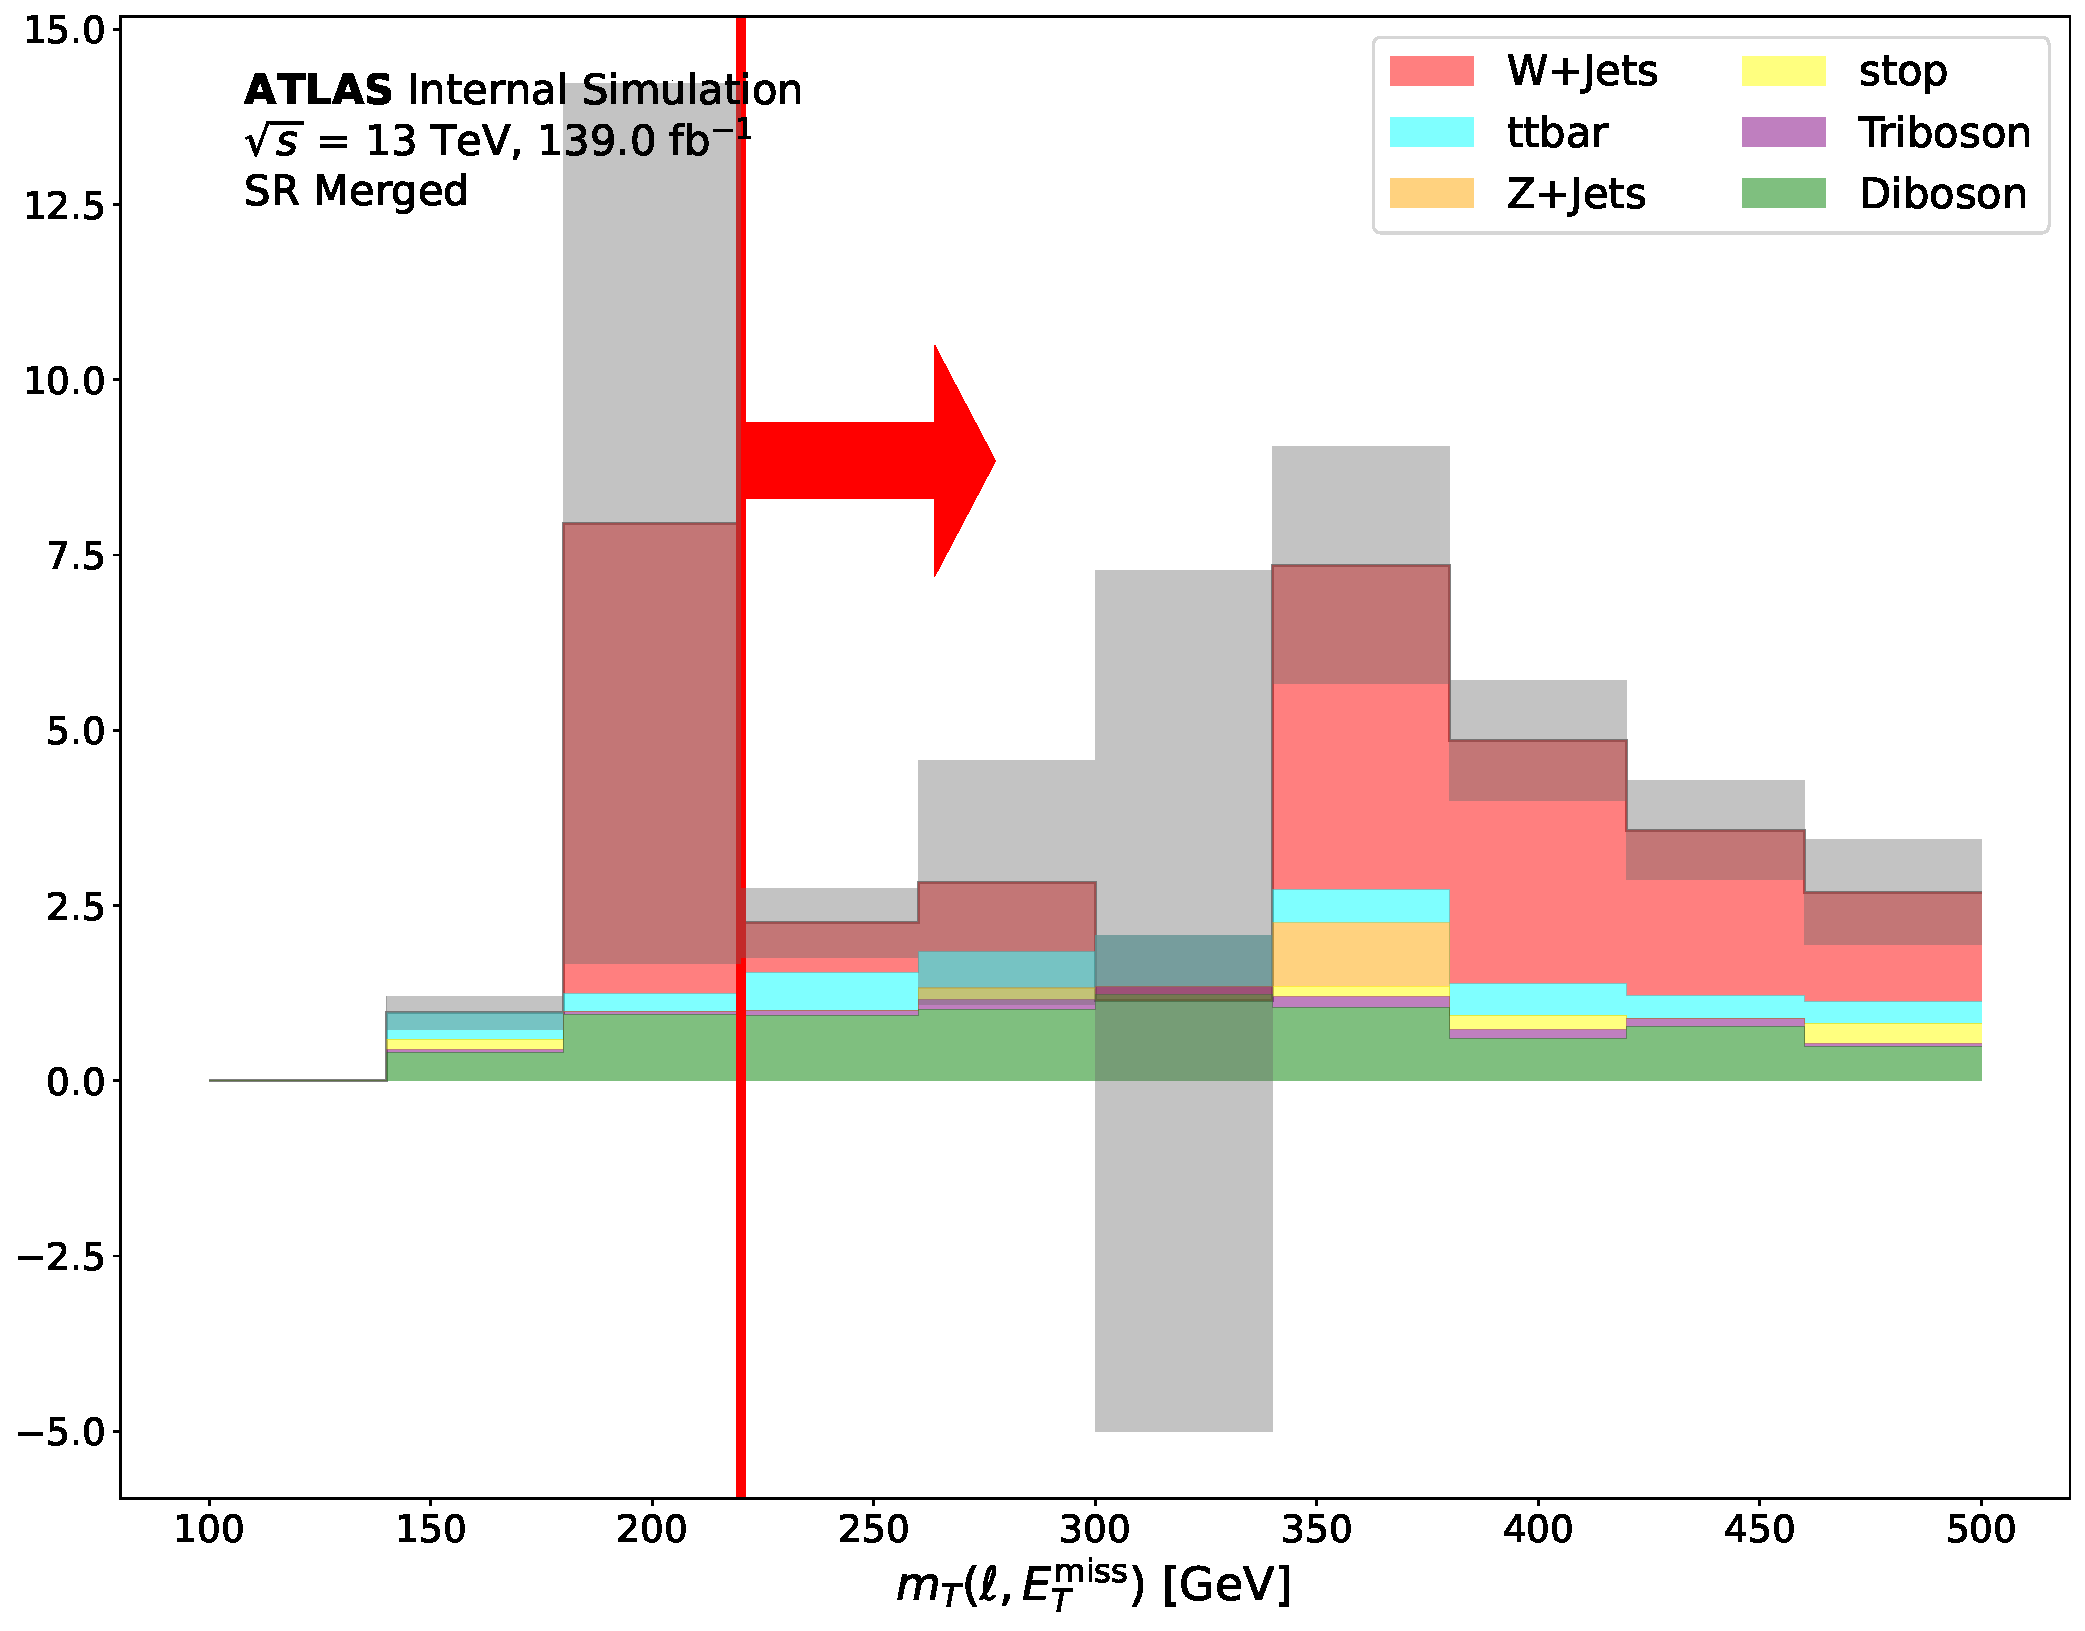
\includegraphics[width = 0.95\textwidth]{Figures/App_SR_CR_distributions/SR1L_Merged/mT_lep_met_N_1.pdf}
    \caption{\mtlepmet (merged SR)}
     \end{subfigure}
    \begin{subfigure}{0.45\textwidth}
     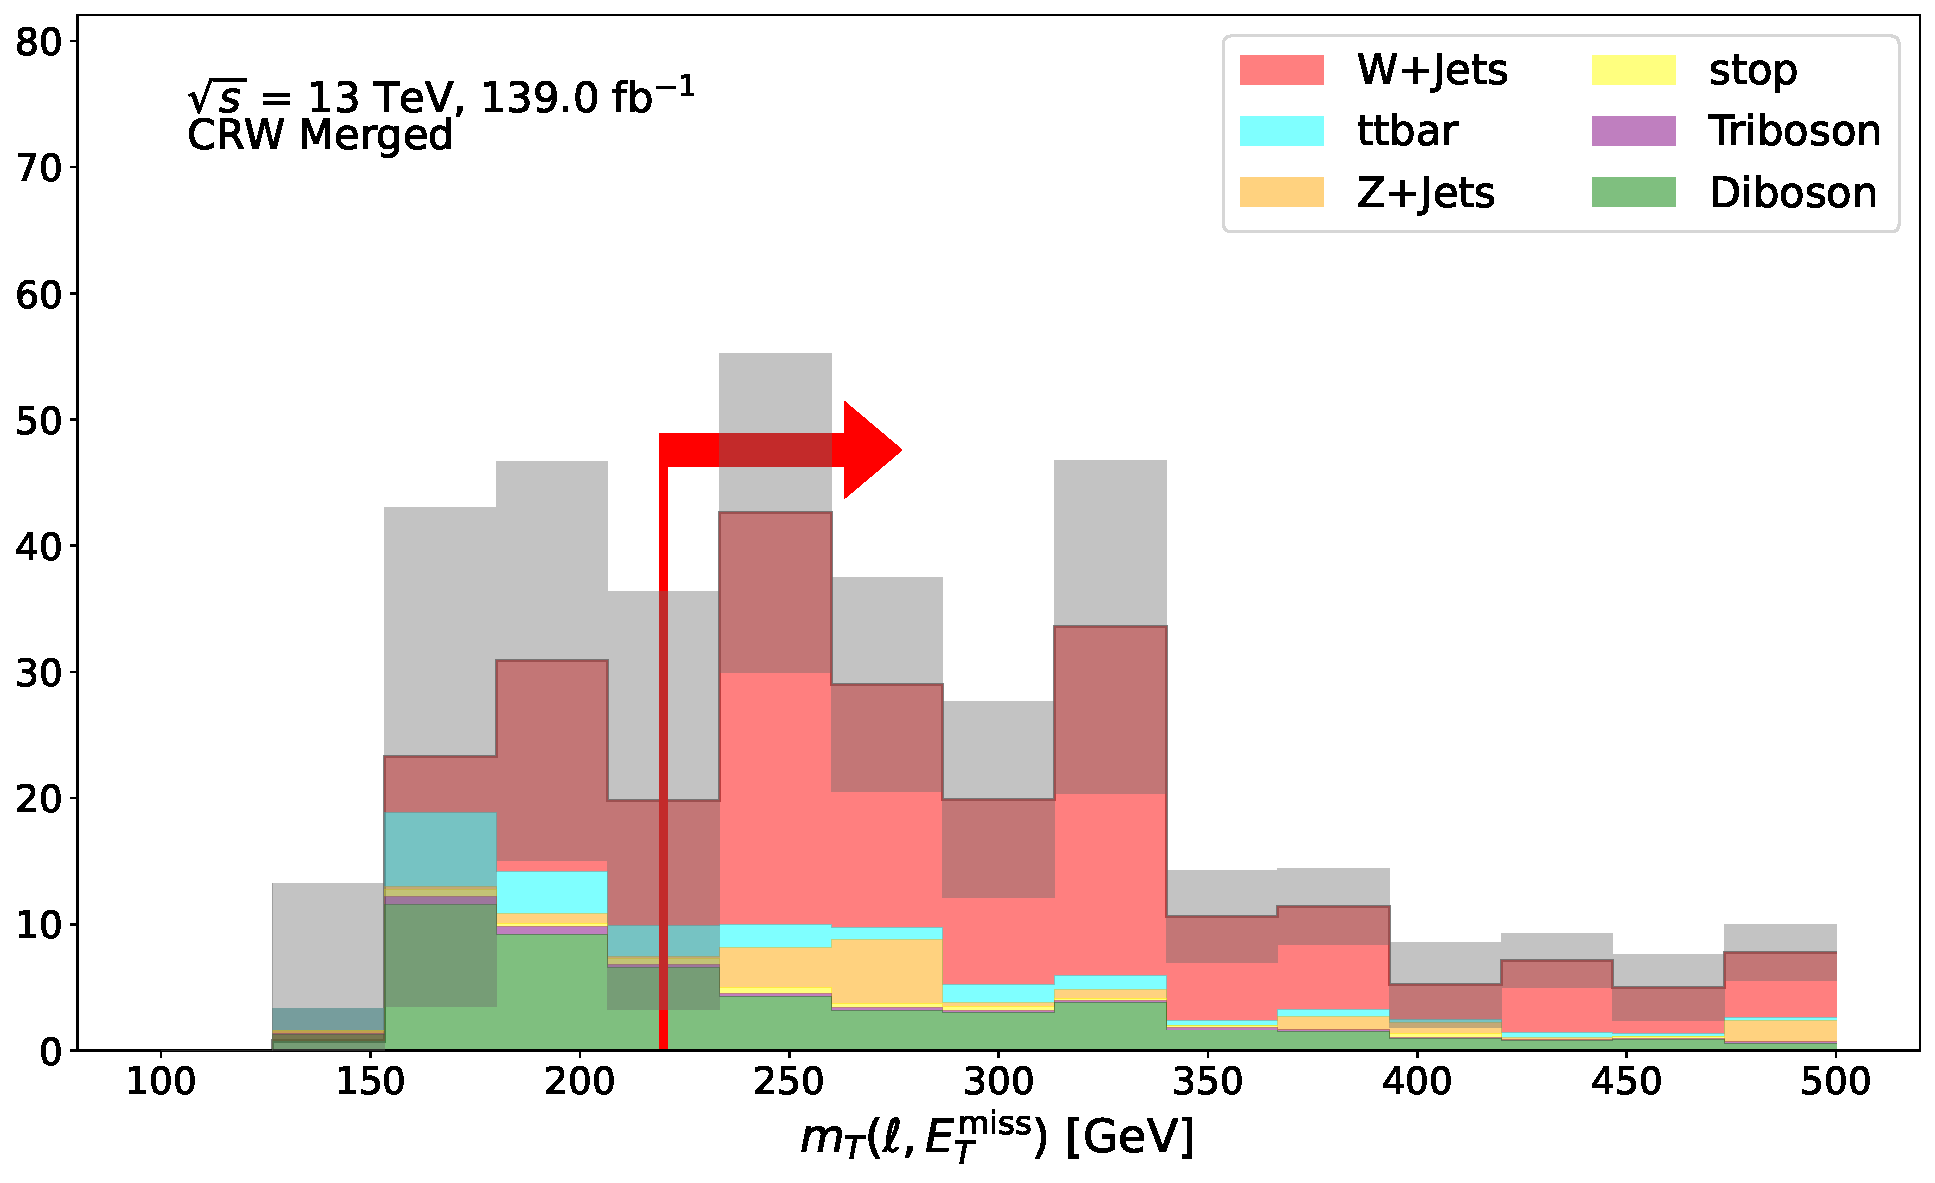
\includegraphics[width = 0.95\textwidth]{Figures/App_SR_CR_distributions/CRW_Merged/mT_lep_met_N_1.pdf}
     \caption{\mtlepmet (merged \wjets CR)}
     \end{subfigure}

      \begin{subfigure}{0.45\textwidth}
     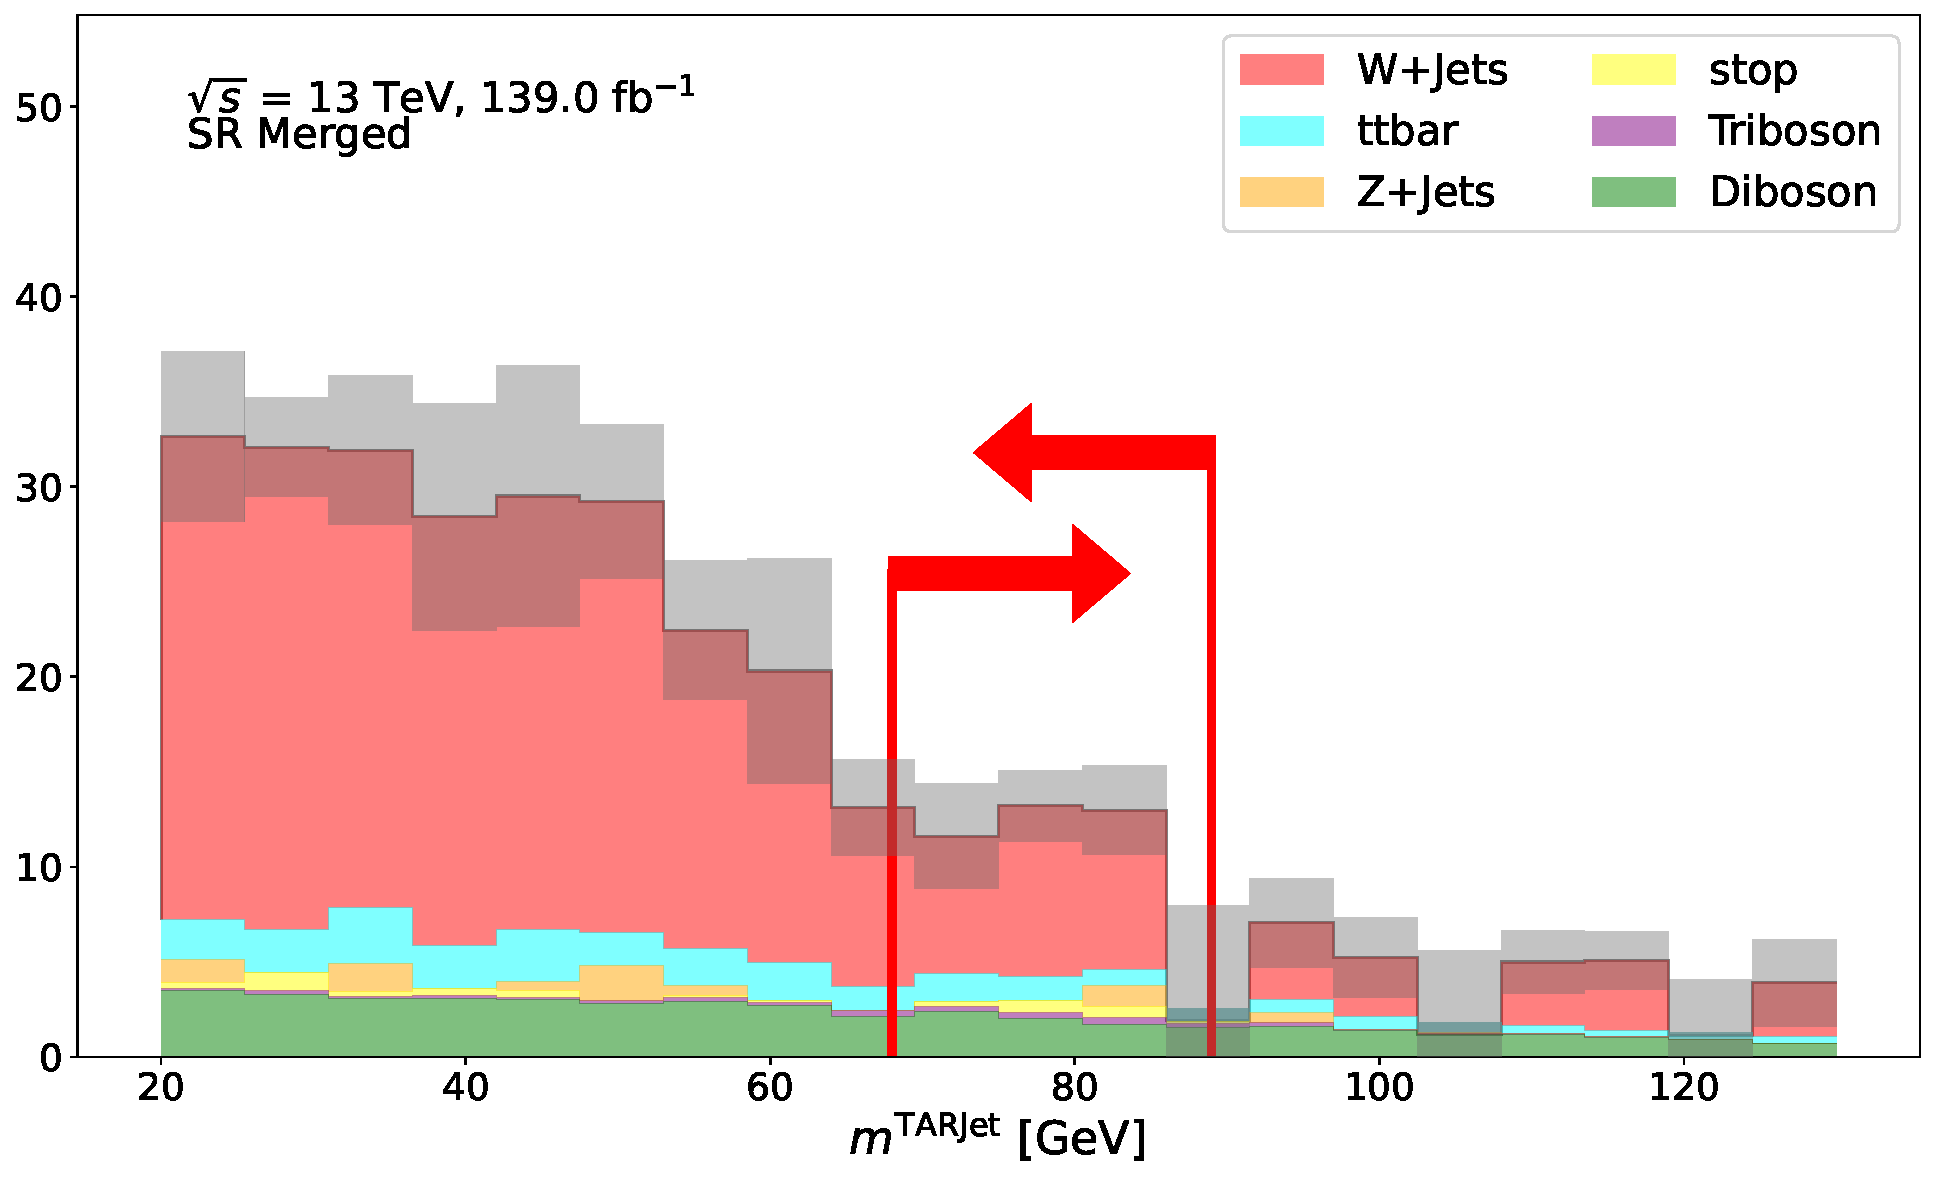
\includegraphics[width = 0.95\textwidth]{Figures/App_SR_CR_distributions/SR1L_Merged/TARJets10_mTAR0_N_1.pdf}
    \caption{\mTAR (merged SR)}
     \end{subfigure}
    \begin{subfigure}{0.45\textwidth}
     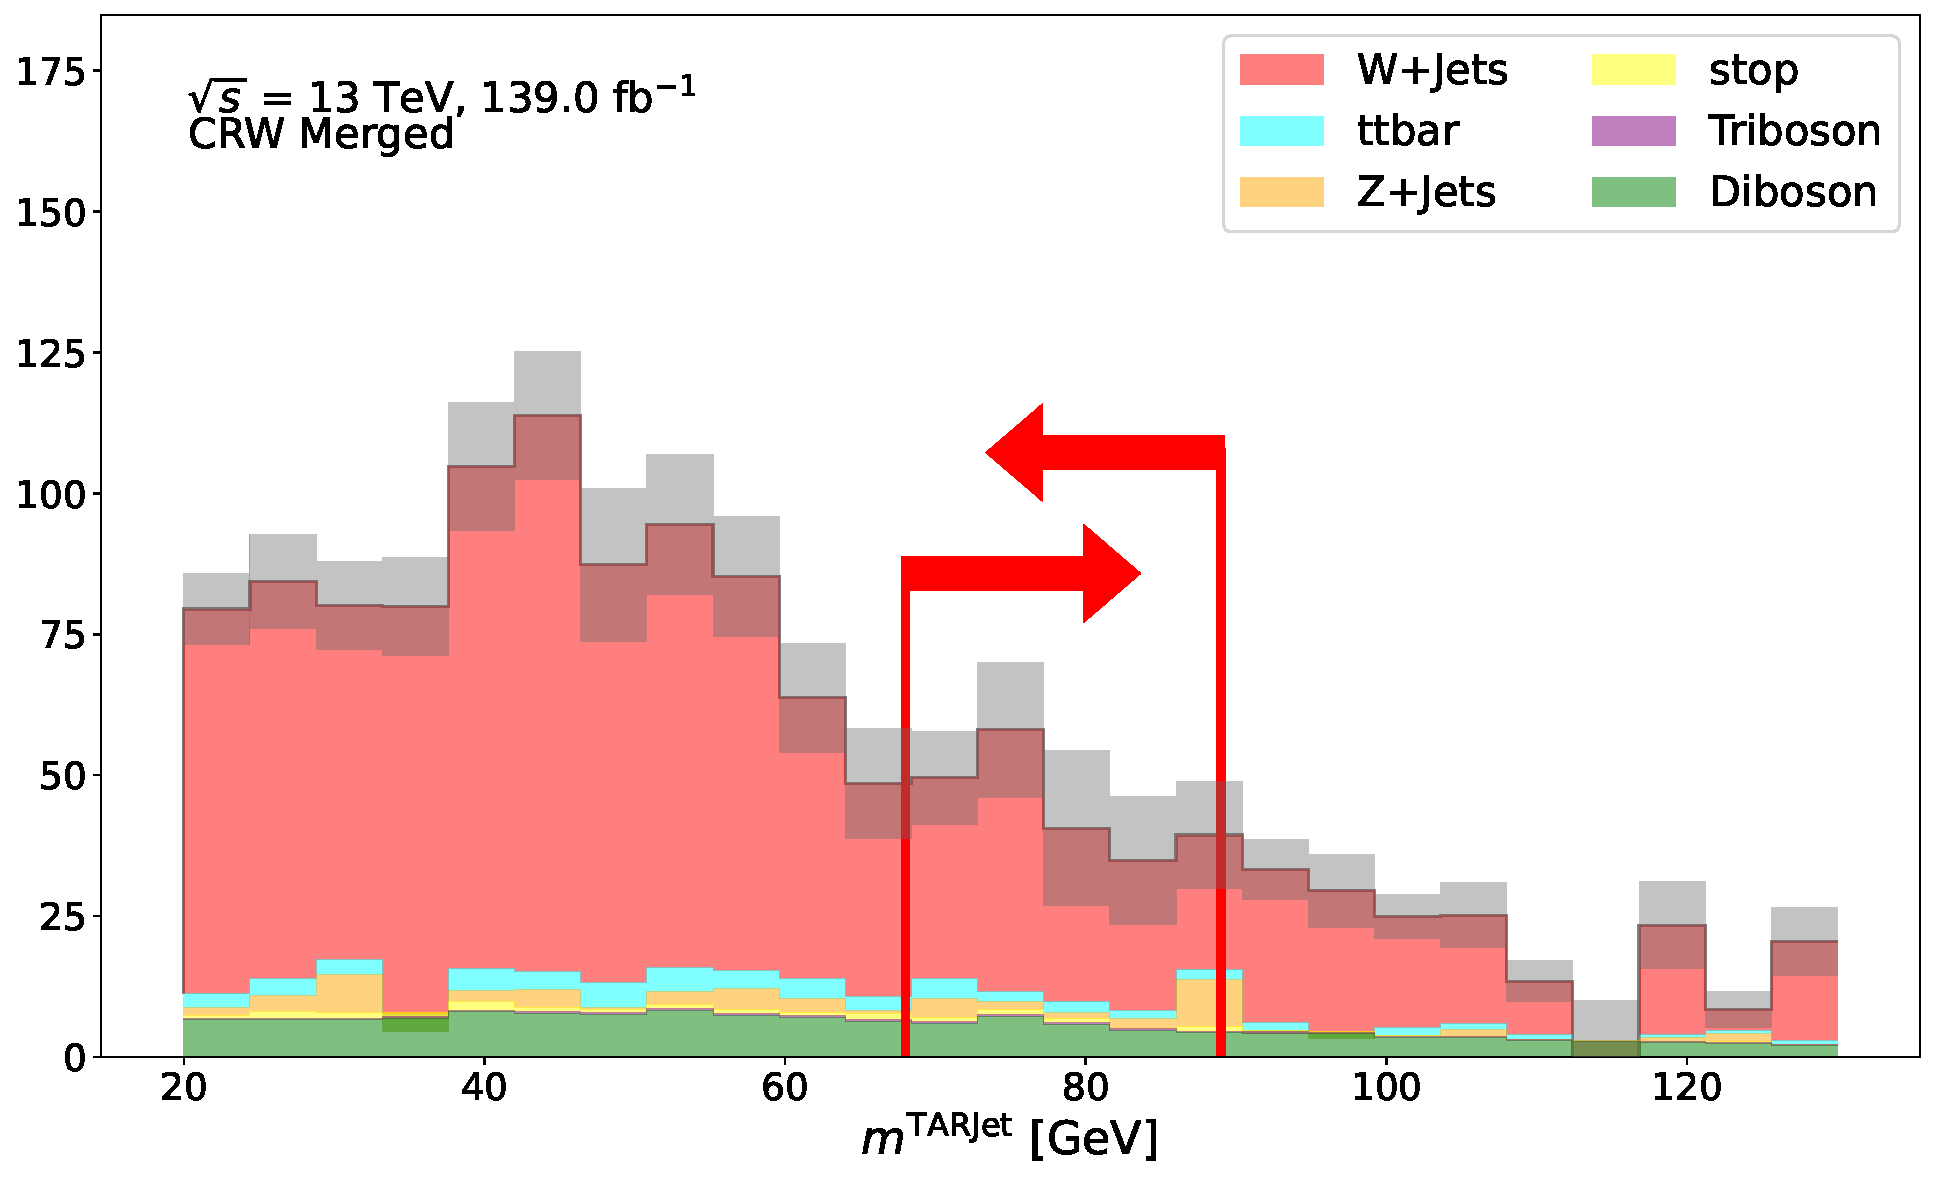
\includegraphics[width = 0.95\textwidth]{Figures/App_SR_CR_distributions/CRW_Merged/TARJets10_mTAR0_N_1.pdf}
     \caption{\mTAR (merged \wjets CR)}
     \end{subfigure}

 \begin{subfigure}{0.45\textwidth}
     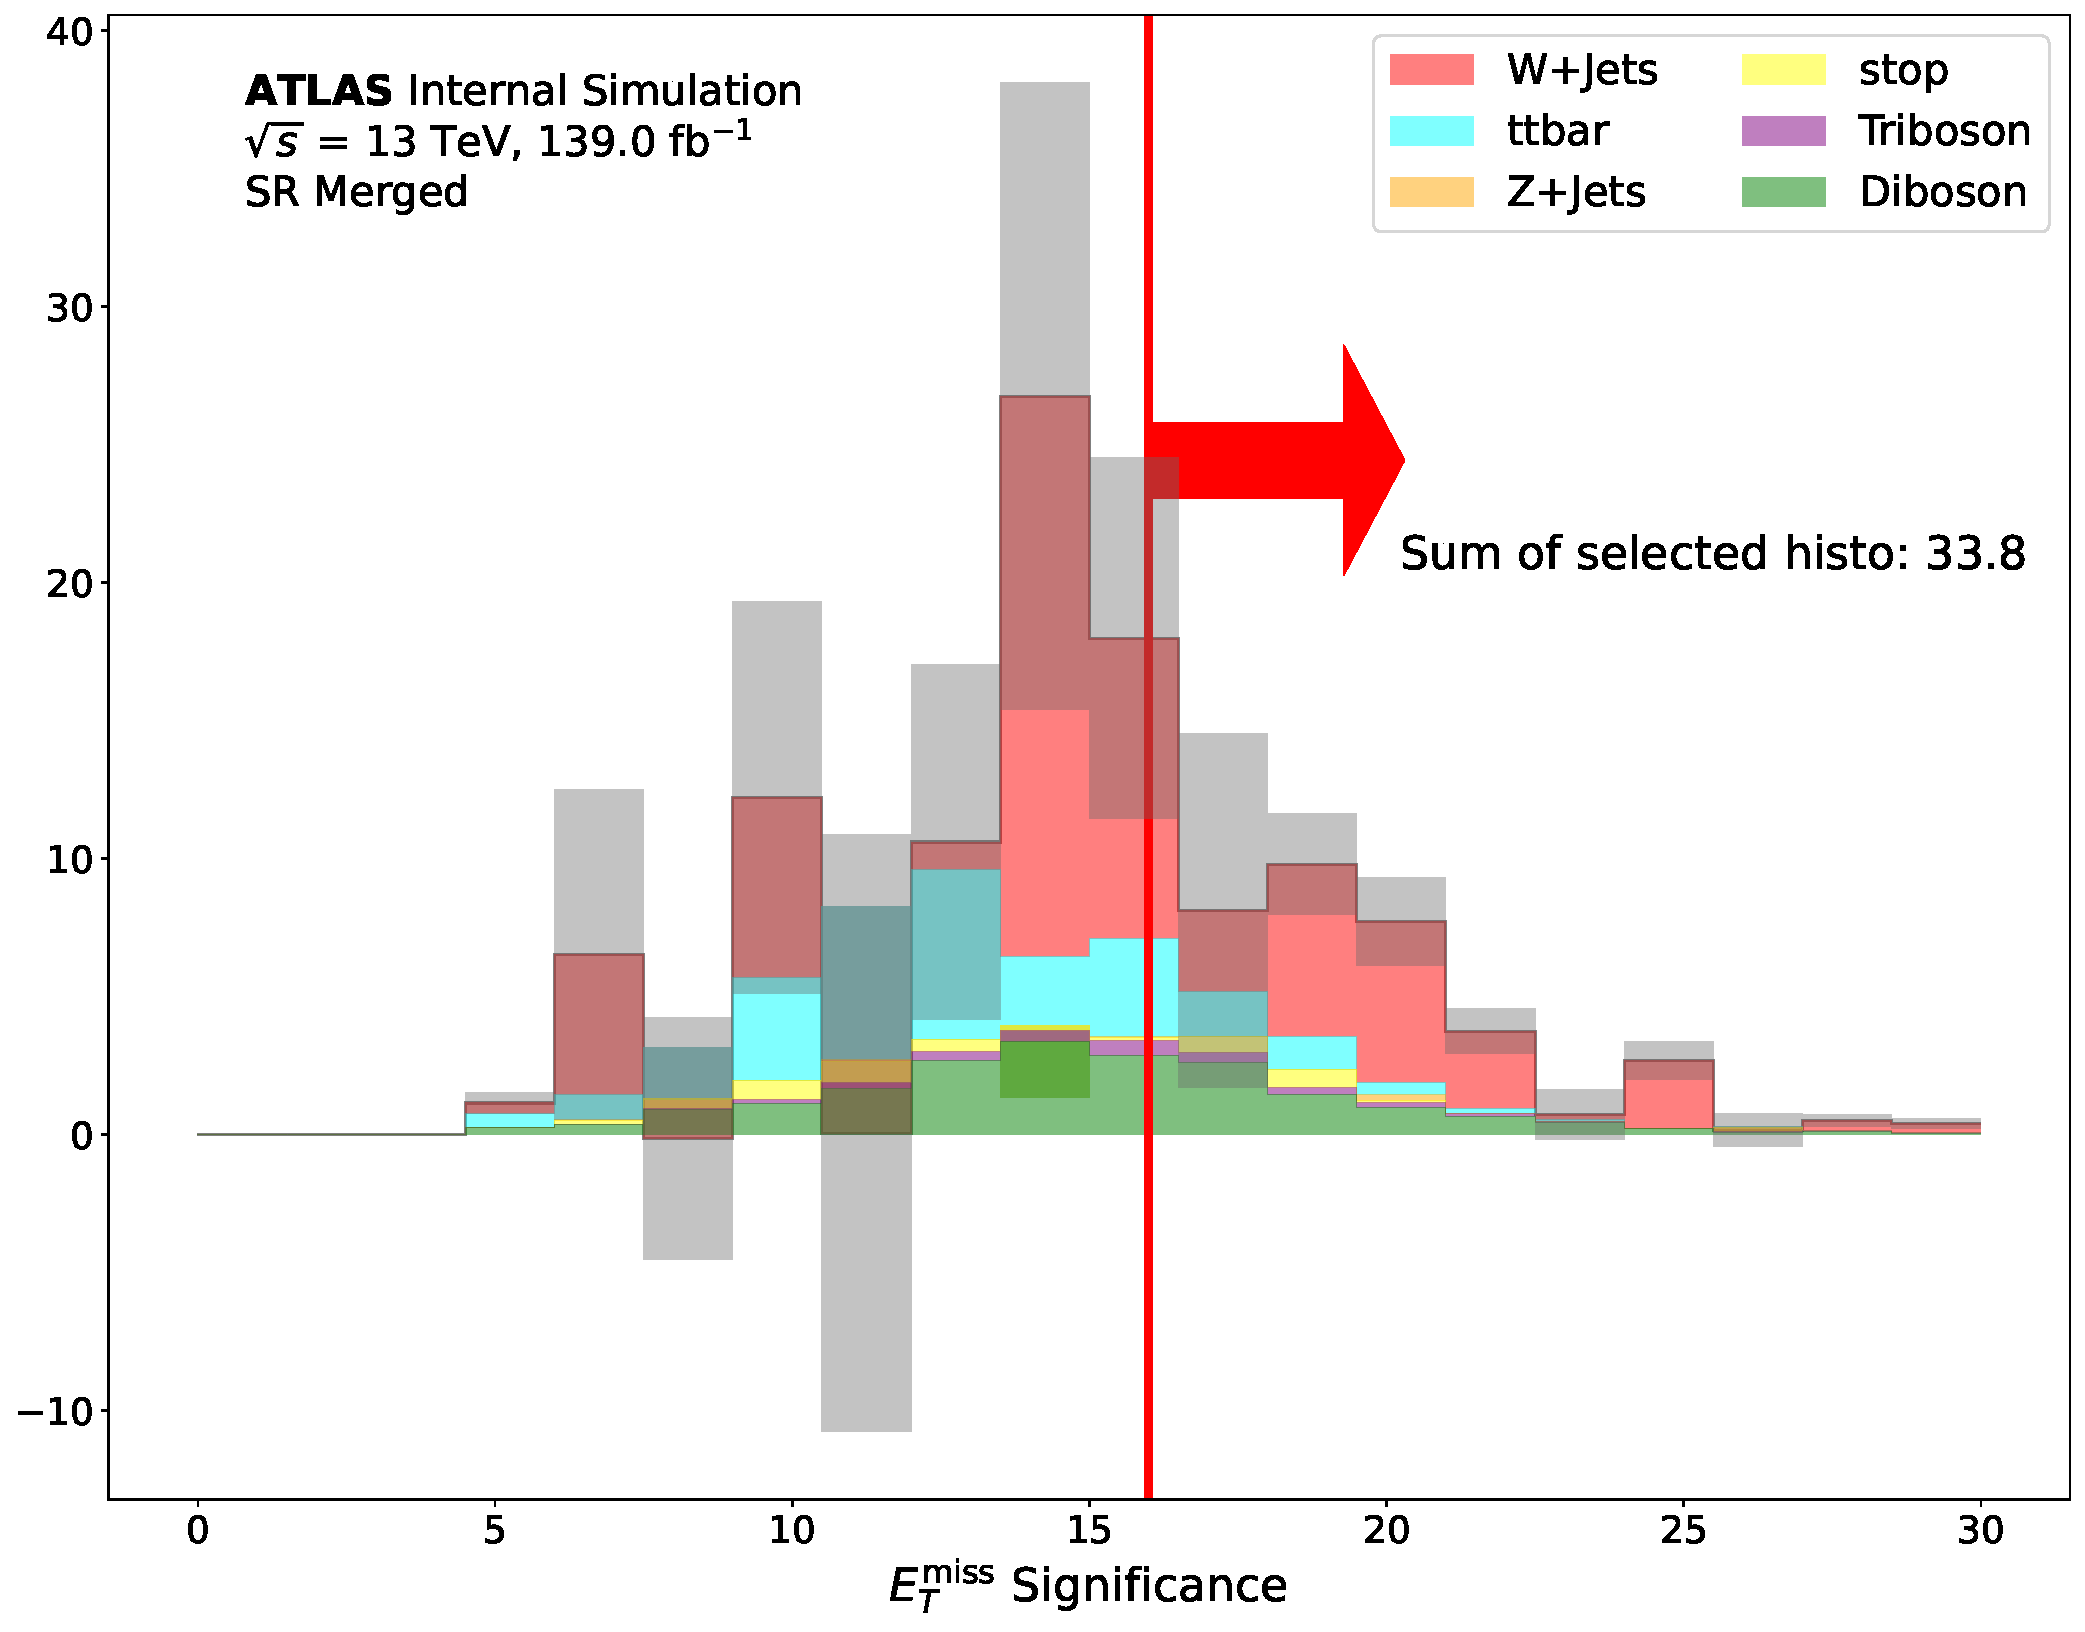
\includegraphics[width = 0.95\textwidth]{Figures/App_SR_CR_distributions/SR1L_Merged/MetTST_Significance_N_1.pdf}
    \caption{\metsig (merged SR)}
     \end{subfigure}
    \begin{subfigure}{0.45\textwidth}
     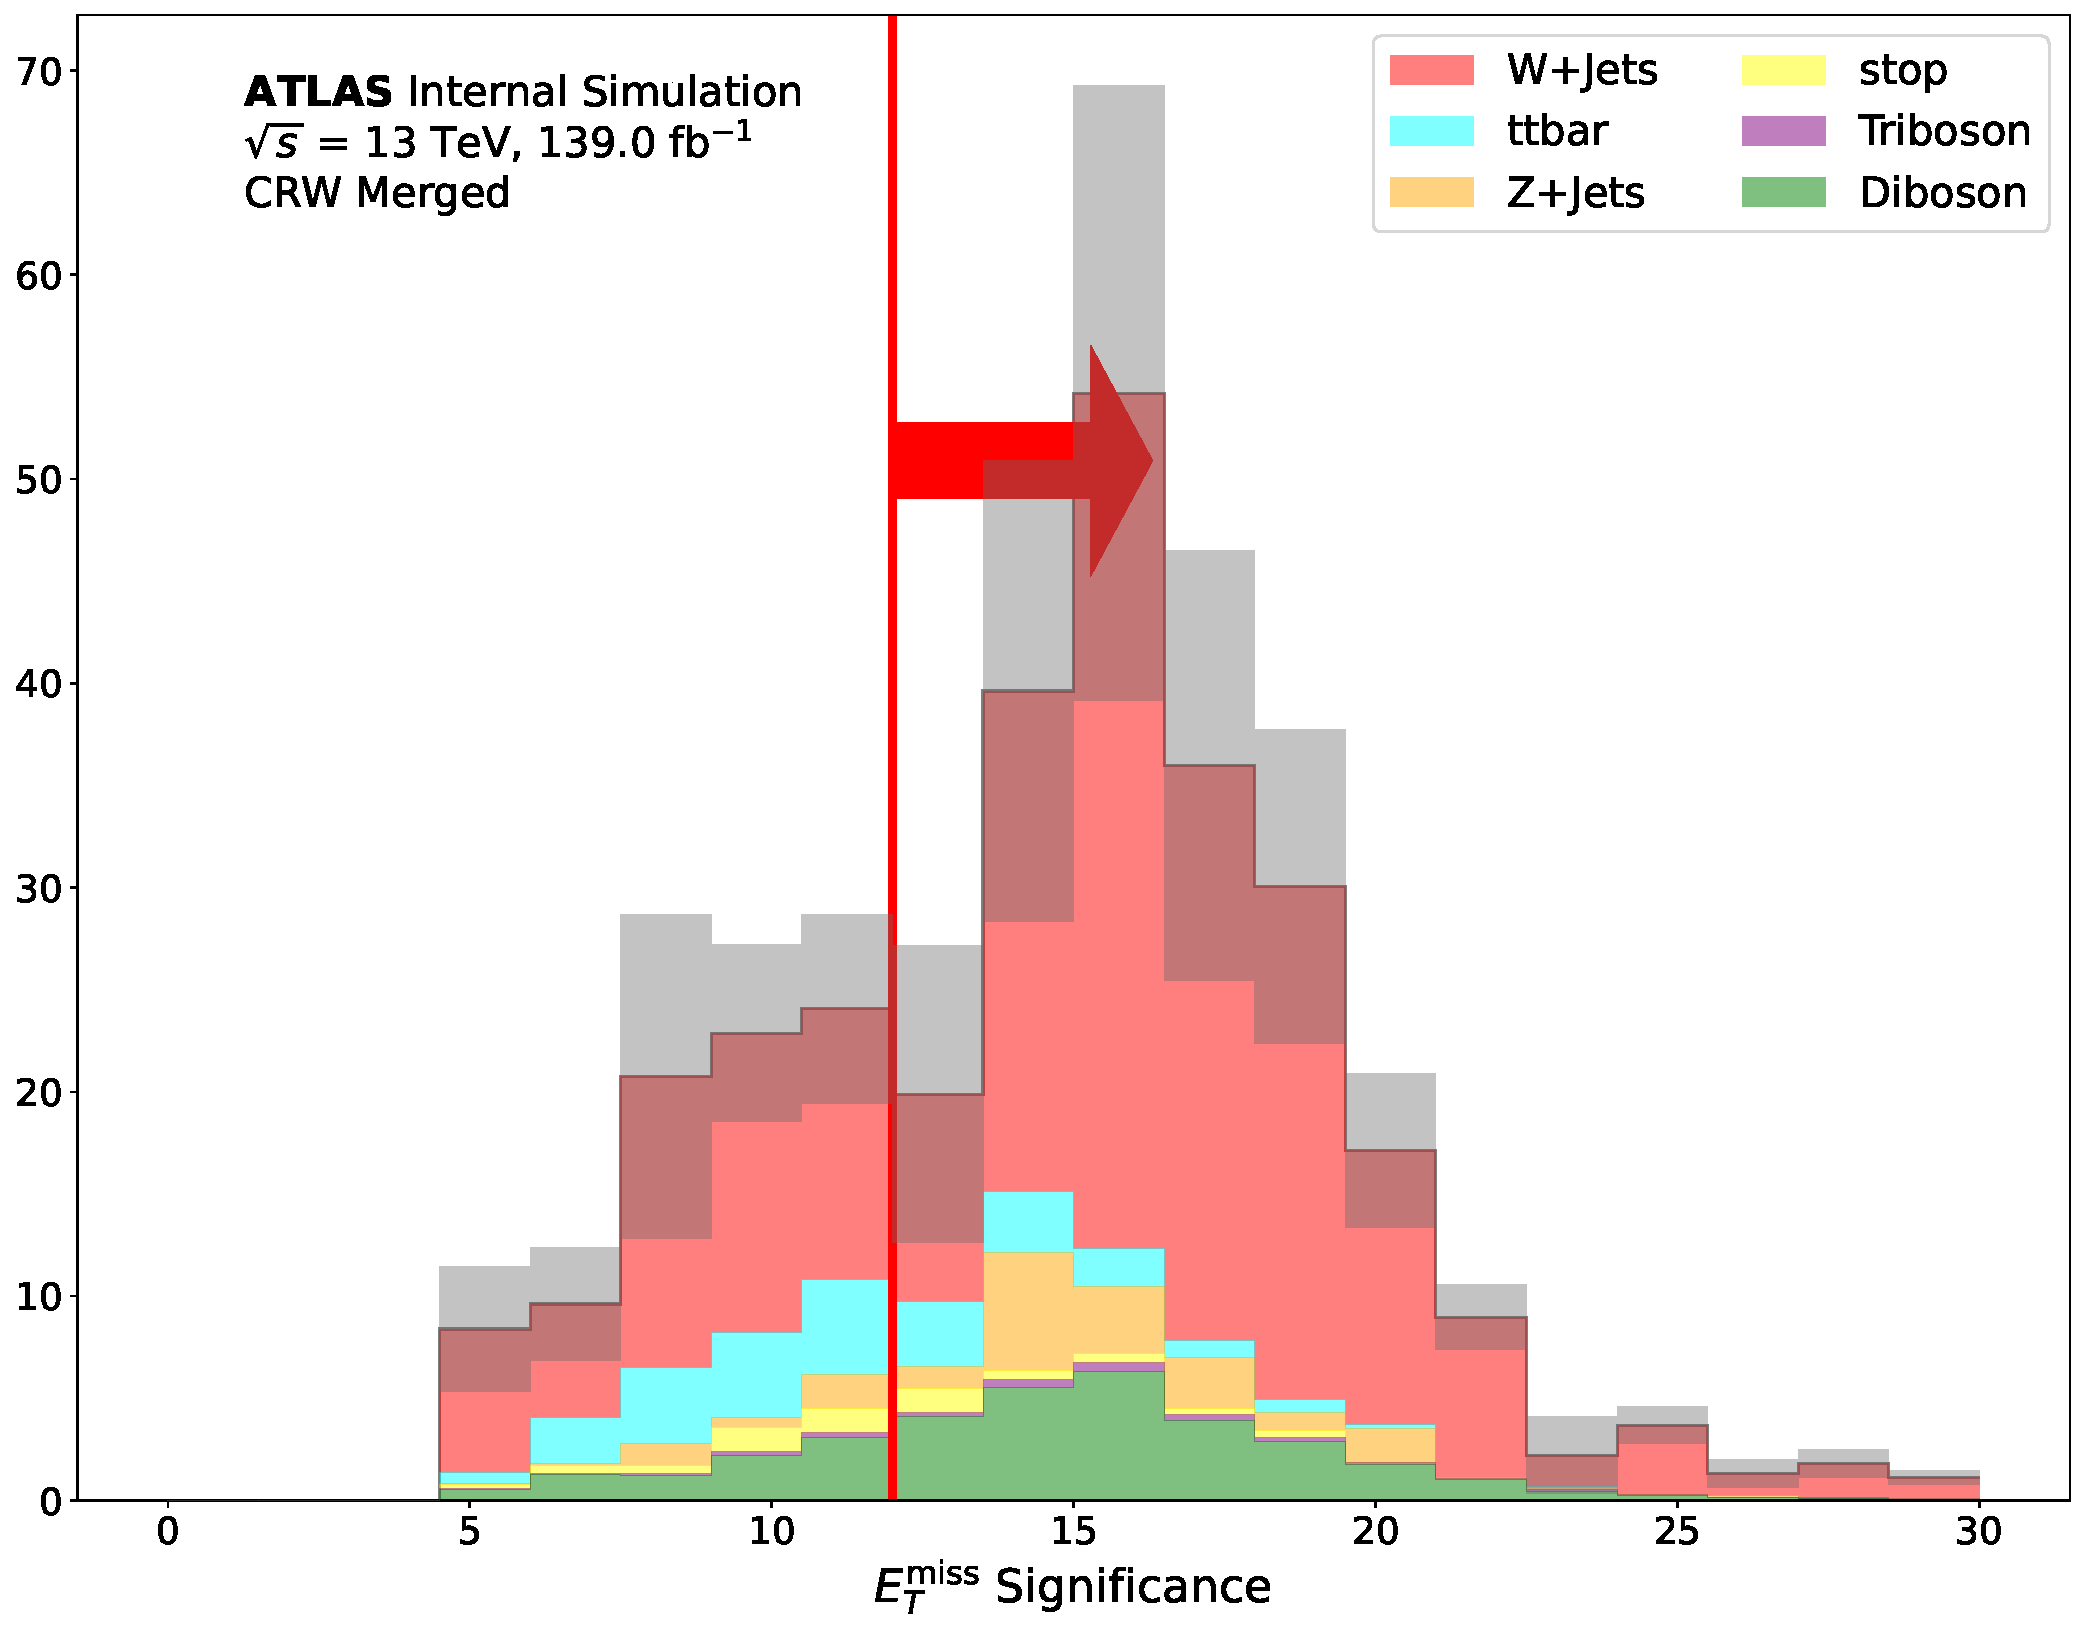
\includegraphics[width = 0.95\textwidth]{Figures/App_SR_CR_distributions/CRW_Merged/MetTST_Significance_N_1.pdf}
     \caption{\metsig (merged \wjets CR)}
     \end{subfigure}
     
     \caption{Comparison of N-1 distributions for kinematic variables of interest between the SR and the \wjets CR in the merged category. Grey bands show statistical uncertainty on the background estimate.}
     \label{fig:N_1_CRW_merged}
  \end{figure}
 \begin{figure}[htbp] \ContinuedFloat
   \begin{subfigure}{0.45\textwidth}
     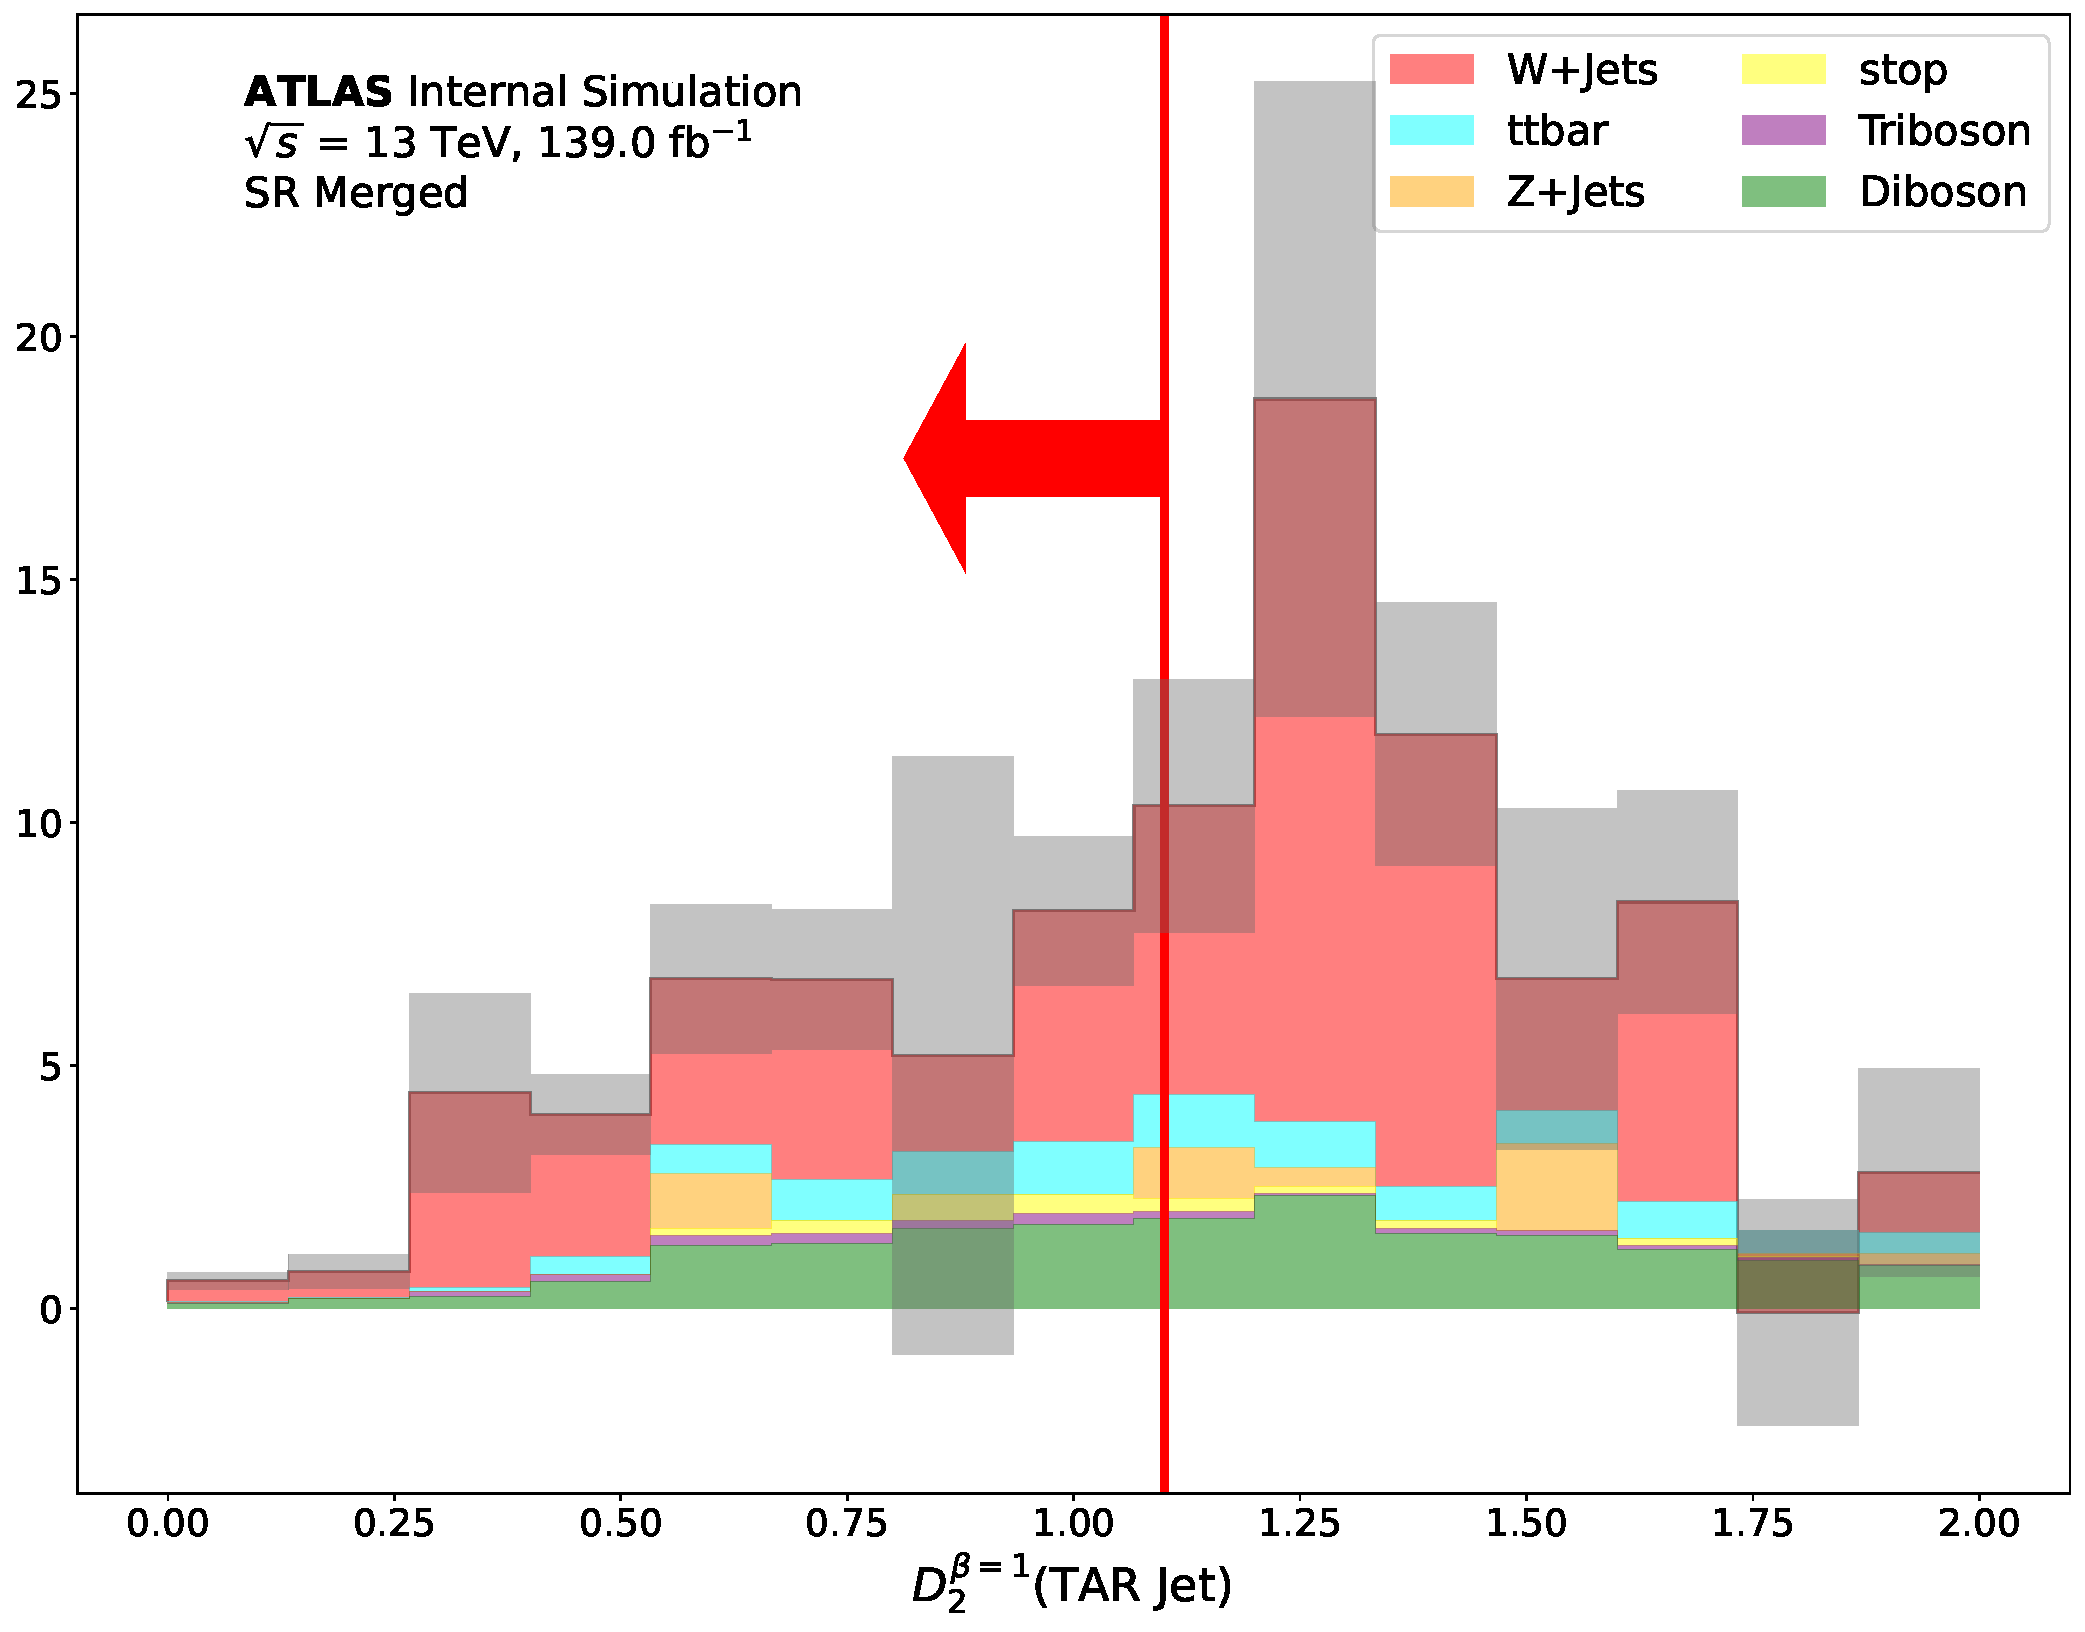
\includegraphics[width = 0.95\textwidth]{Figures/App_SR_CR_distributions/SR1L_Merged/TARJets10_TAR_D20_N_1.pdf}
    \caption{\DtwoTAR (merged SR)}
     \end{subfigure}
    \begin{subfigure}{0.45\textwidth}
     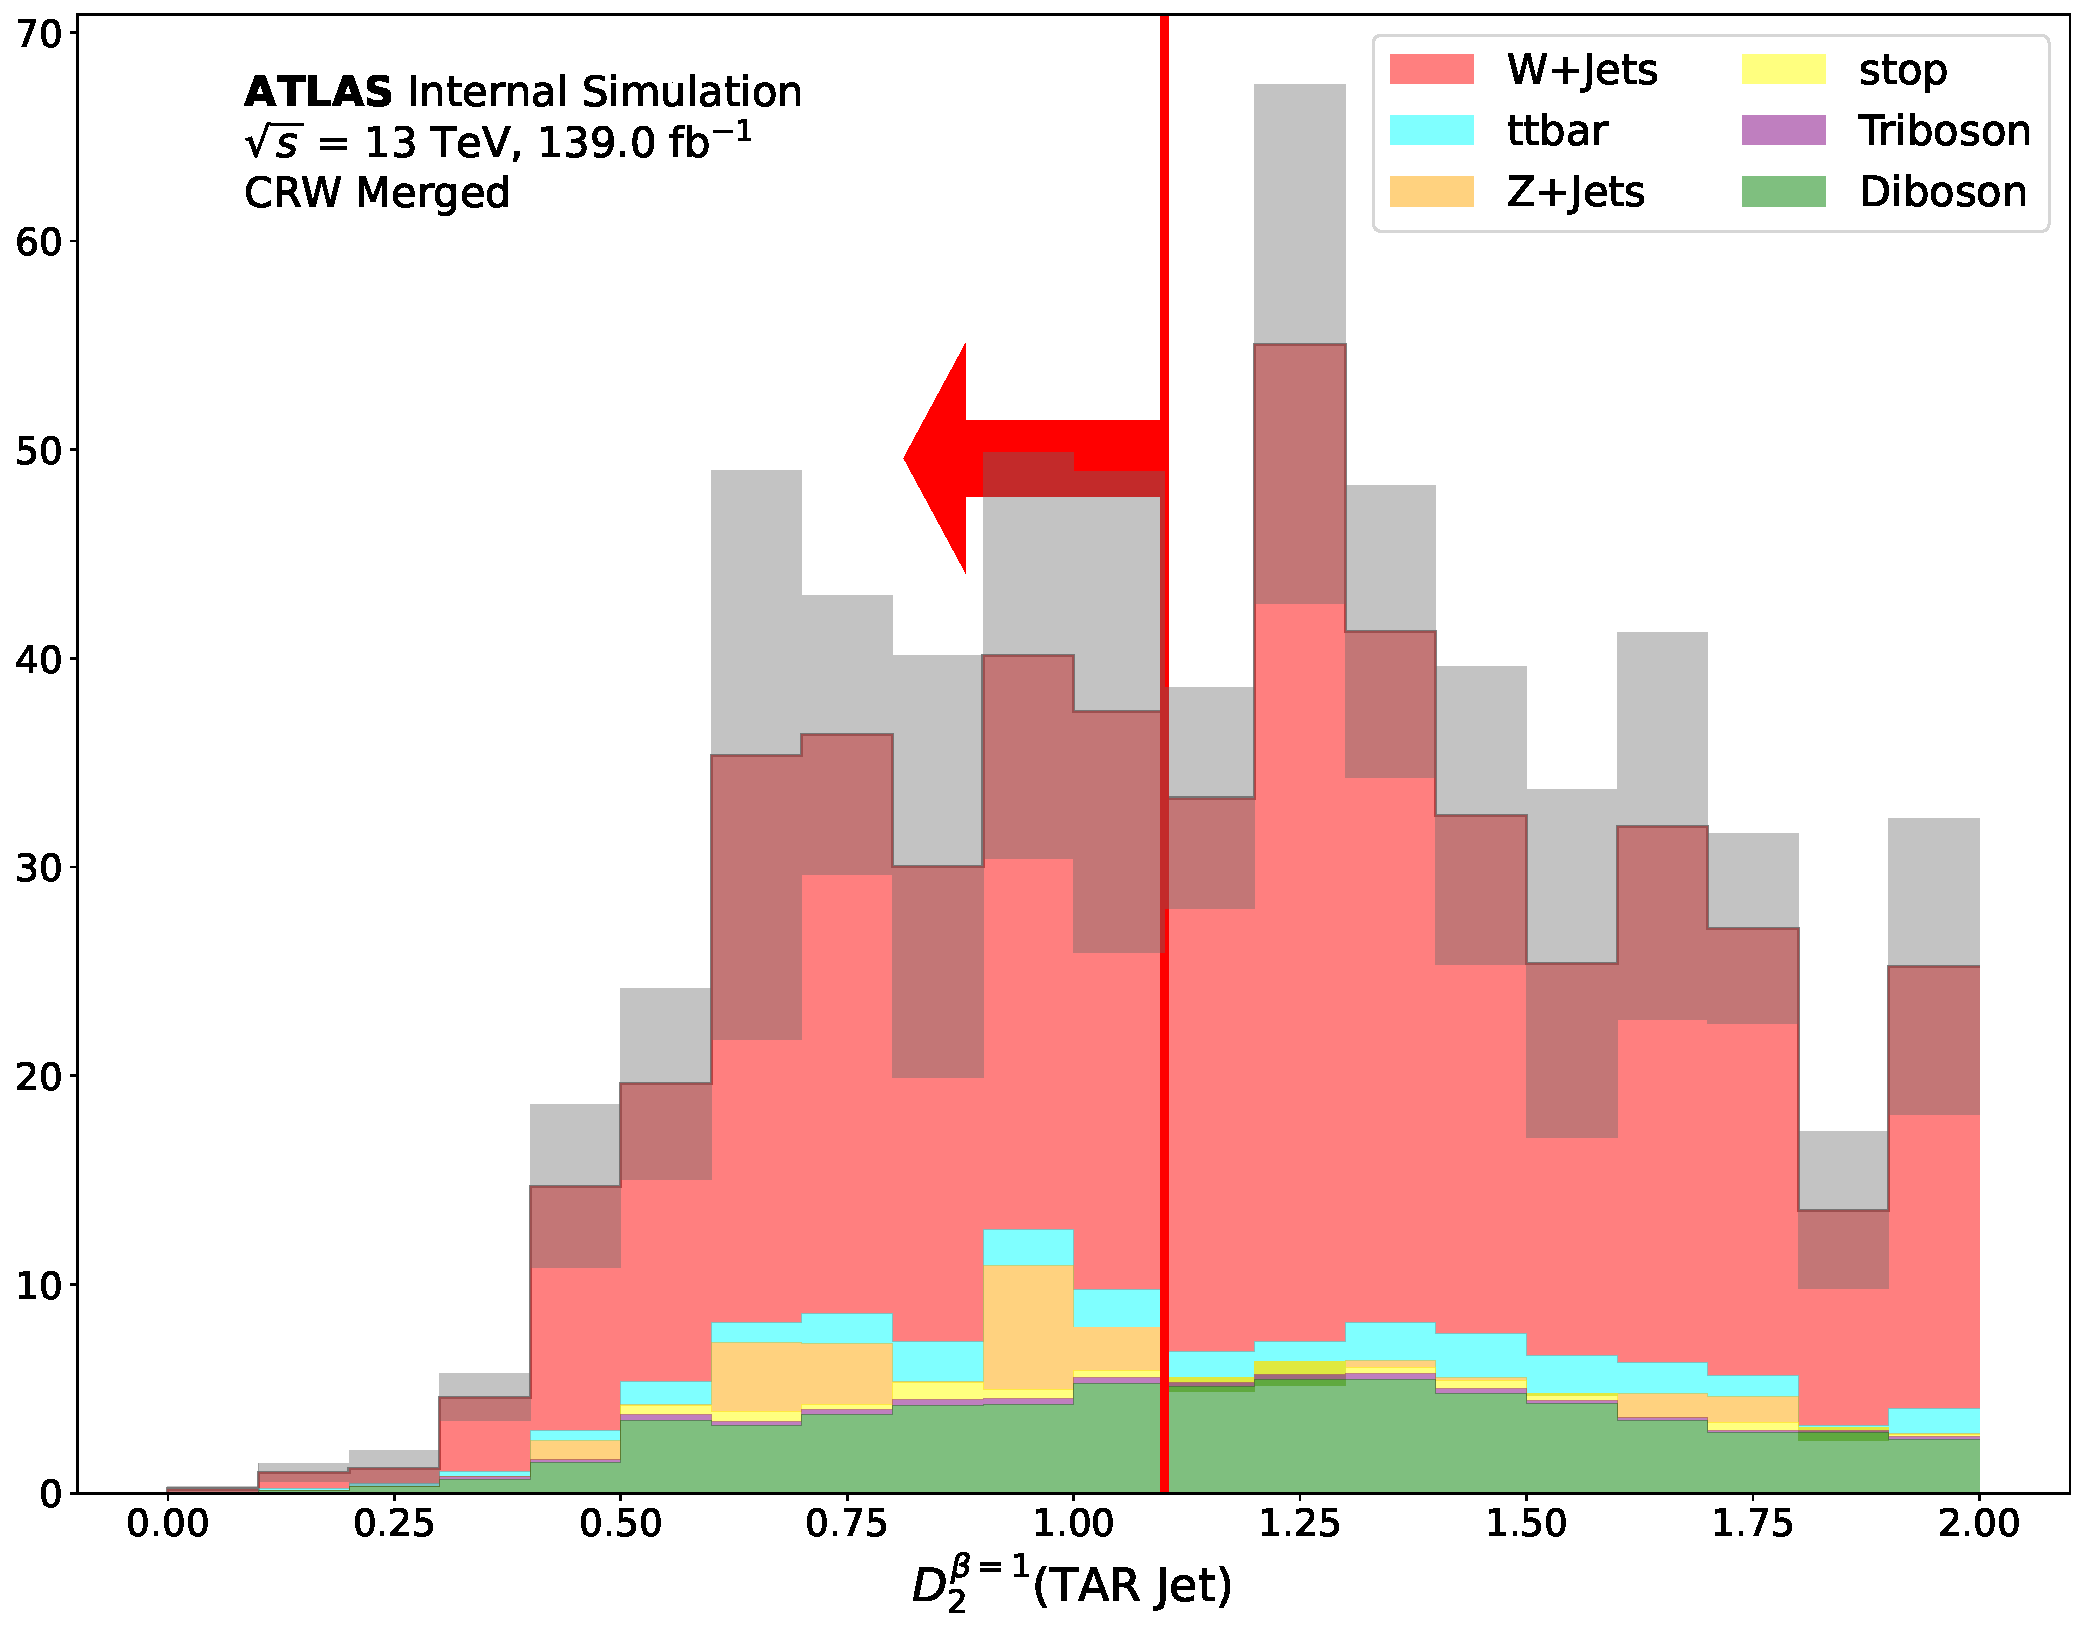
\includegraphics[width = 0.95\textwidth]{Figures/App_SR_CR_distributions/CRW_Merged/TARJets10_TAR_D20_N_1.pdf}
     \caption{\DtwoTAR (merged \wjets CR)}
     \end{subfigure}

   \begin{subfigure}{0.45\textwidth}
     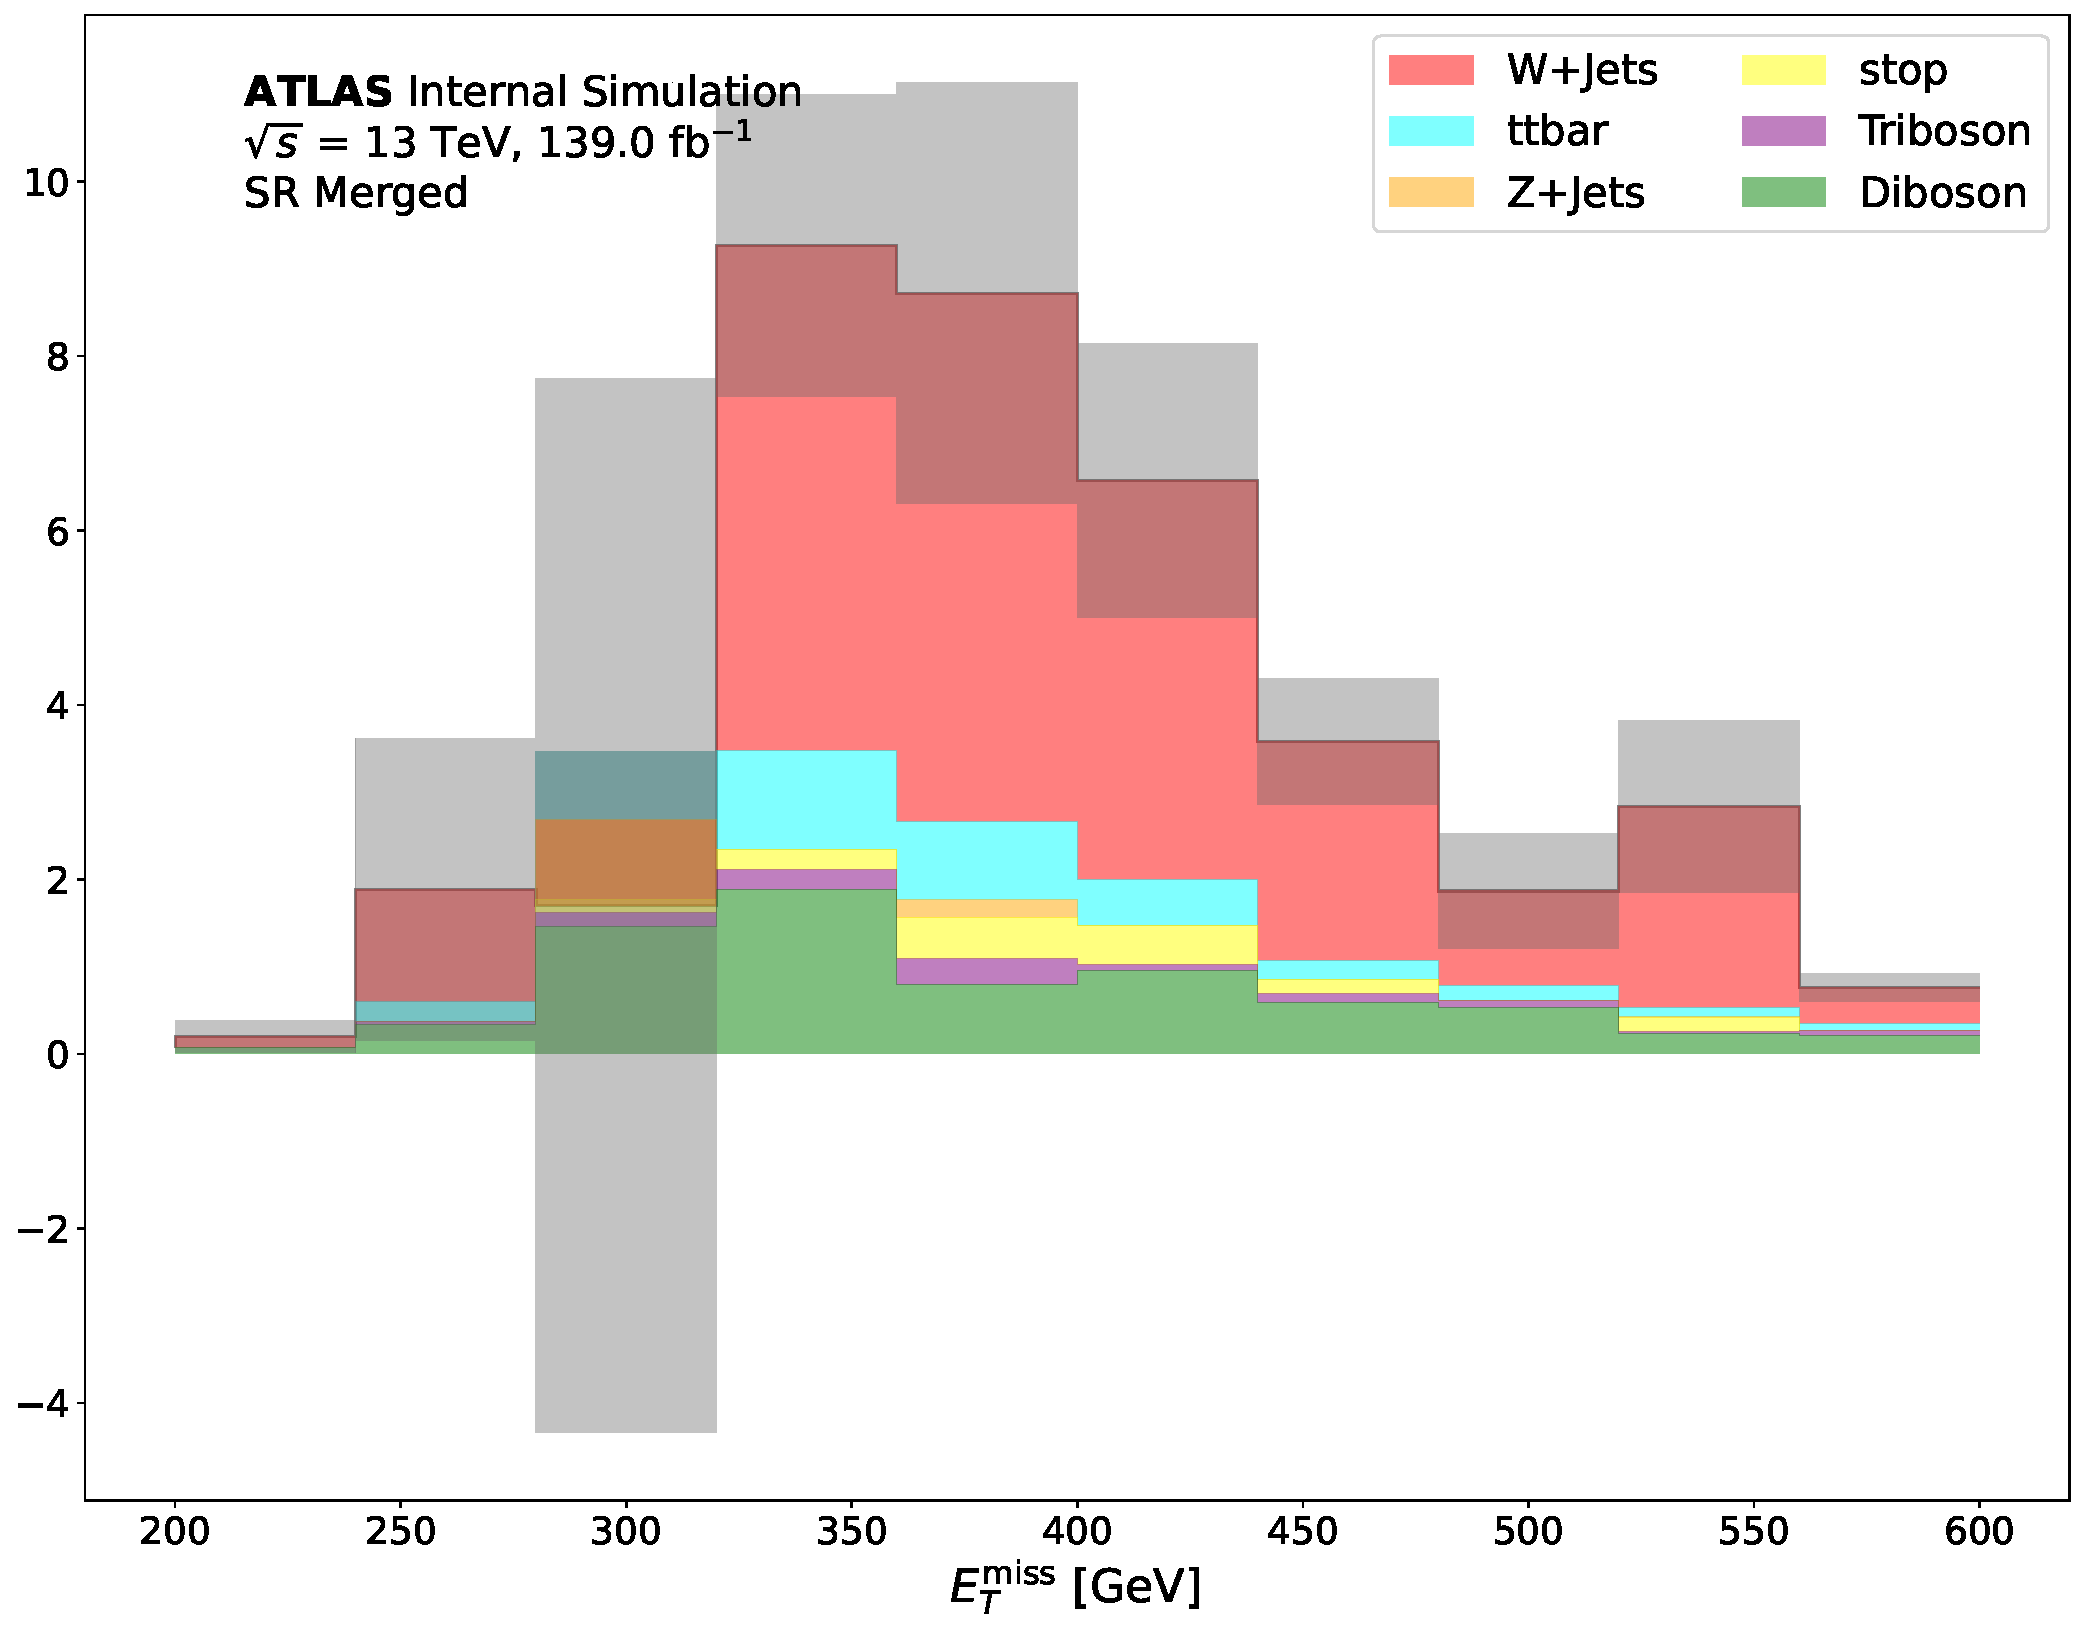
\includegraphics[width = 0.95\textwidth]{Figures/App_SR_CR_distributions/SR1L_Merged/MetTST_met_N_1.pdf}
    \caption{\met (merged SR)}
    \label{fig:N_1_SR_merged_met}
     \end{subfigure}
    \begin{subfigure}{0.45\textwidth}
     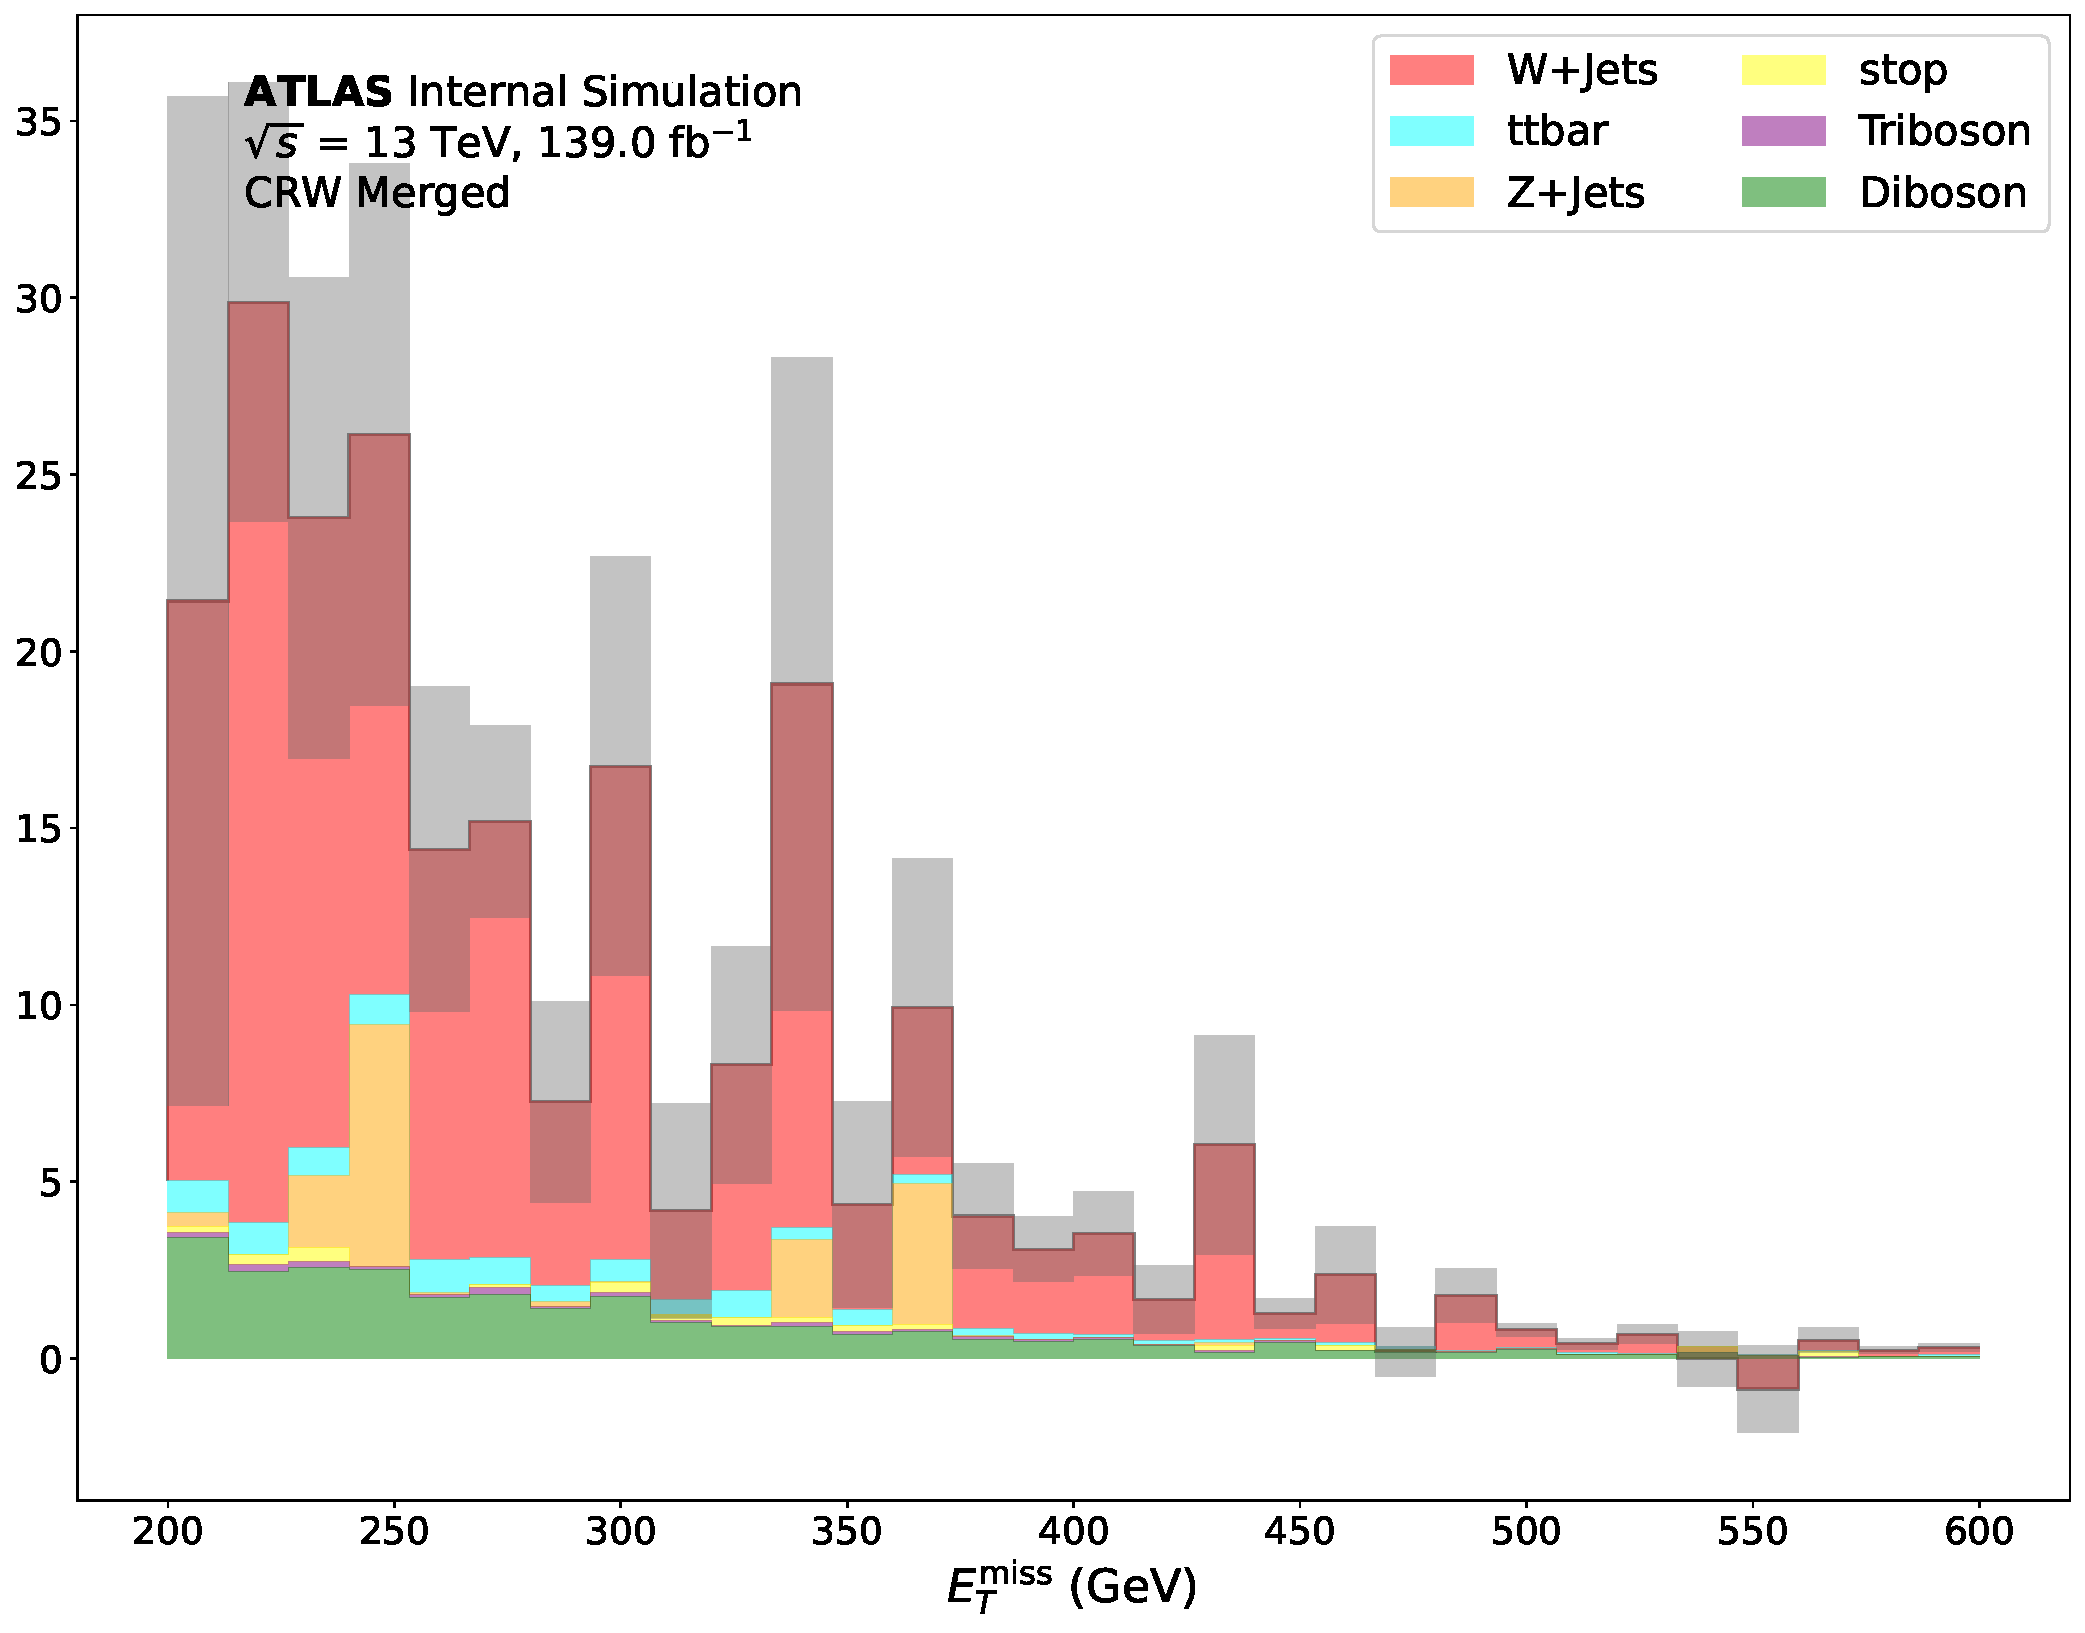
\includegraphics[width = 0.95\textwidth]{Figures/App_SR_CR_distributions/CRW_Merged/MetTST_met_N_1.pdf}
     \caption{\met (merged \wjets CR)}
     \label{fig:N_1_CRW_merged_met}
     \end{subfigure}
     \caption{Comparison of N-1 distributions for kinematic variables of interest between the SR and the \wjets CR in the merged category (continued).}
  \end{figure}
  

  \begin{figure}[htbp]
  \centering
     \begin{subfigure}{0.45\textwidth}
     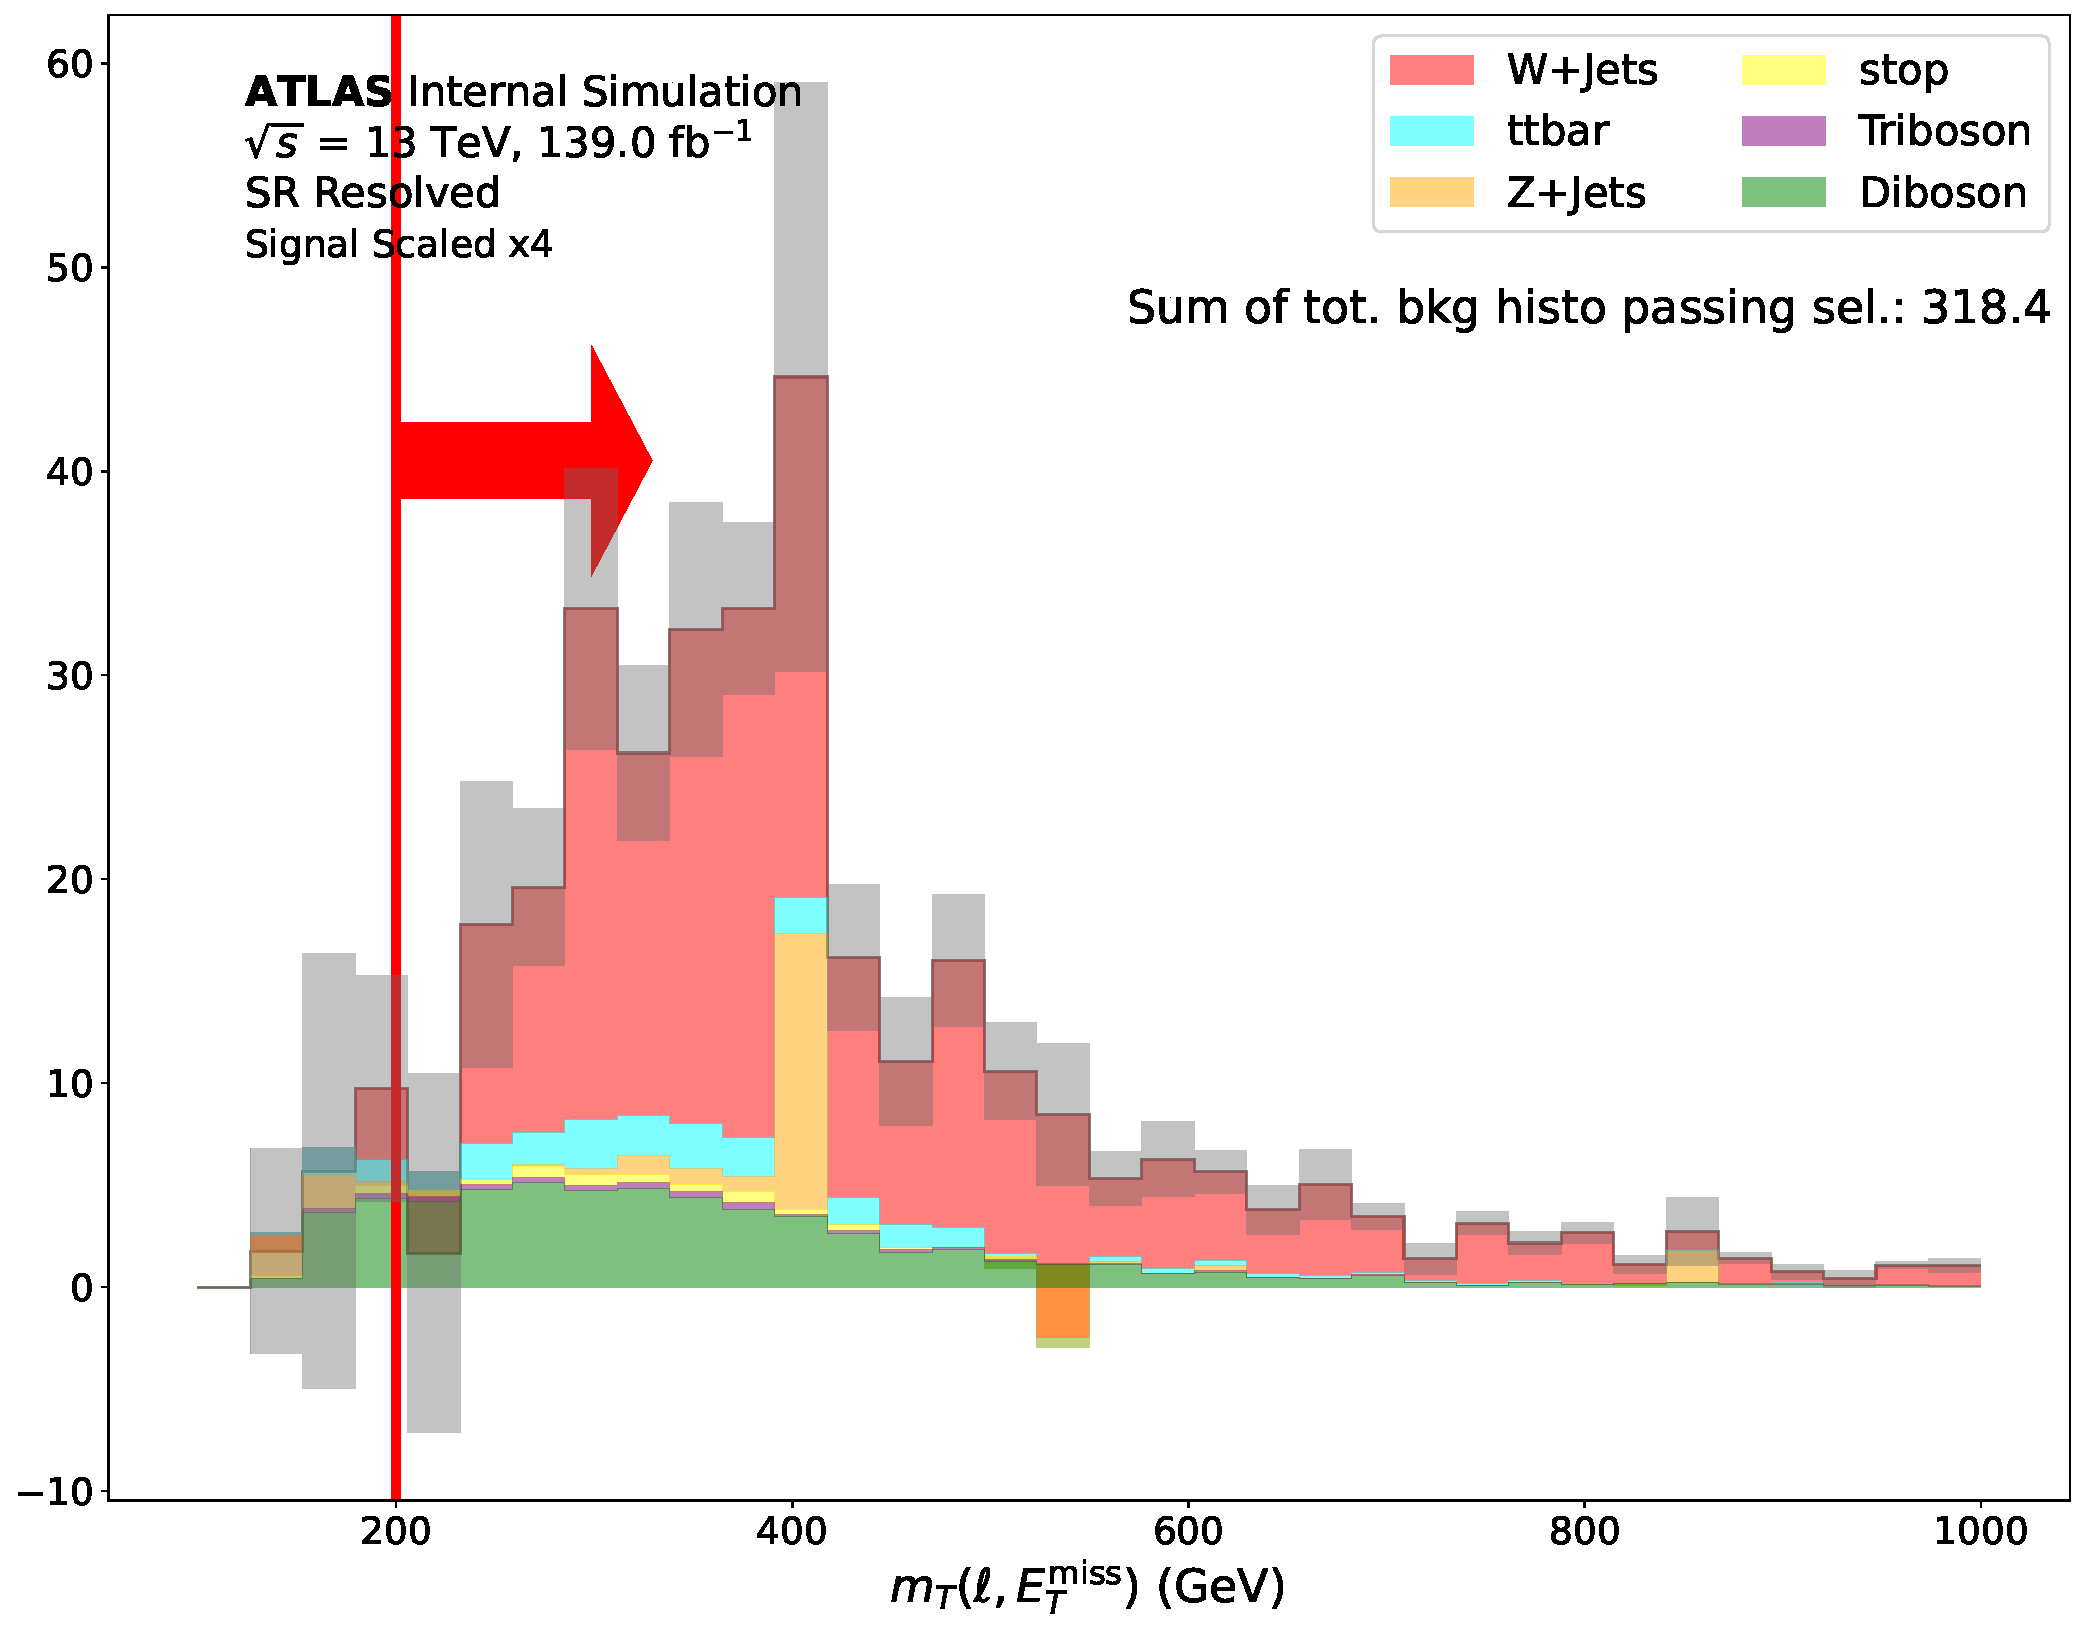
\includegraphics[width = 0.95\textwidth]{Figures/App_SR_CR_distributions/SR1L_Resolved/mT_lep_met_N_1.pdf}
    \caption{\mtlepmet (resolved SR)}
     \end{subfigure}
    \begin{subfigure}{0.45\textwidth}
     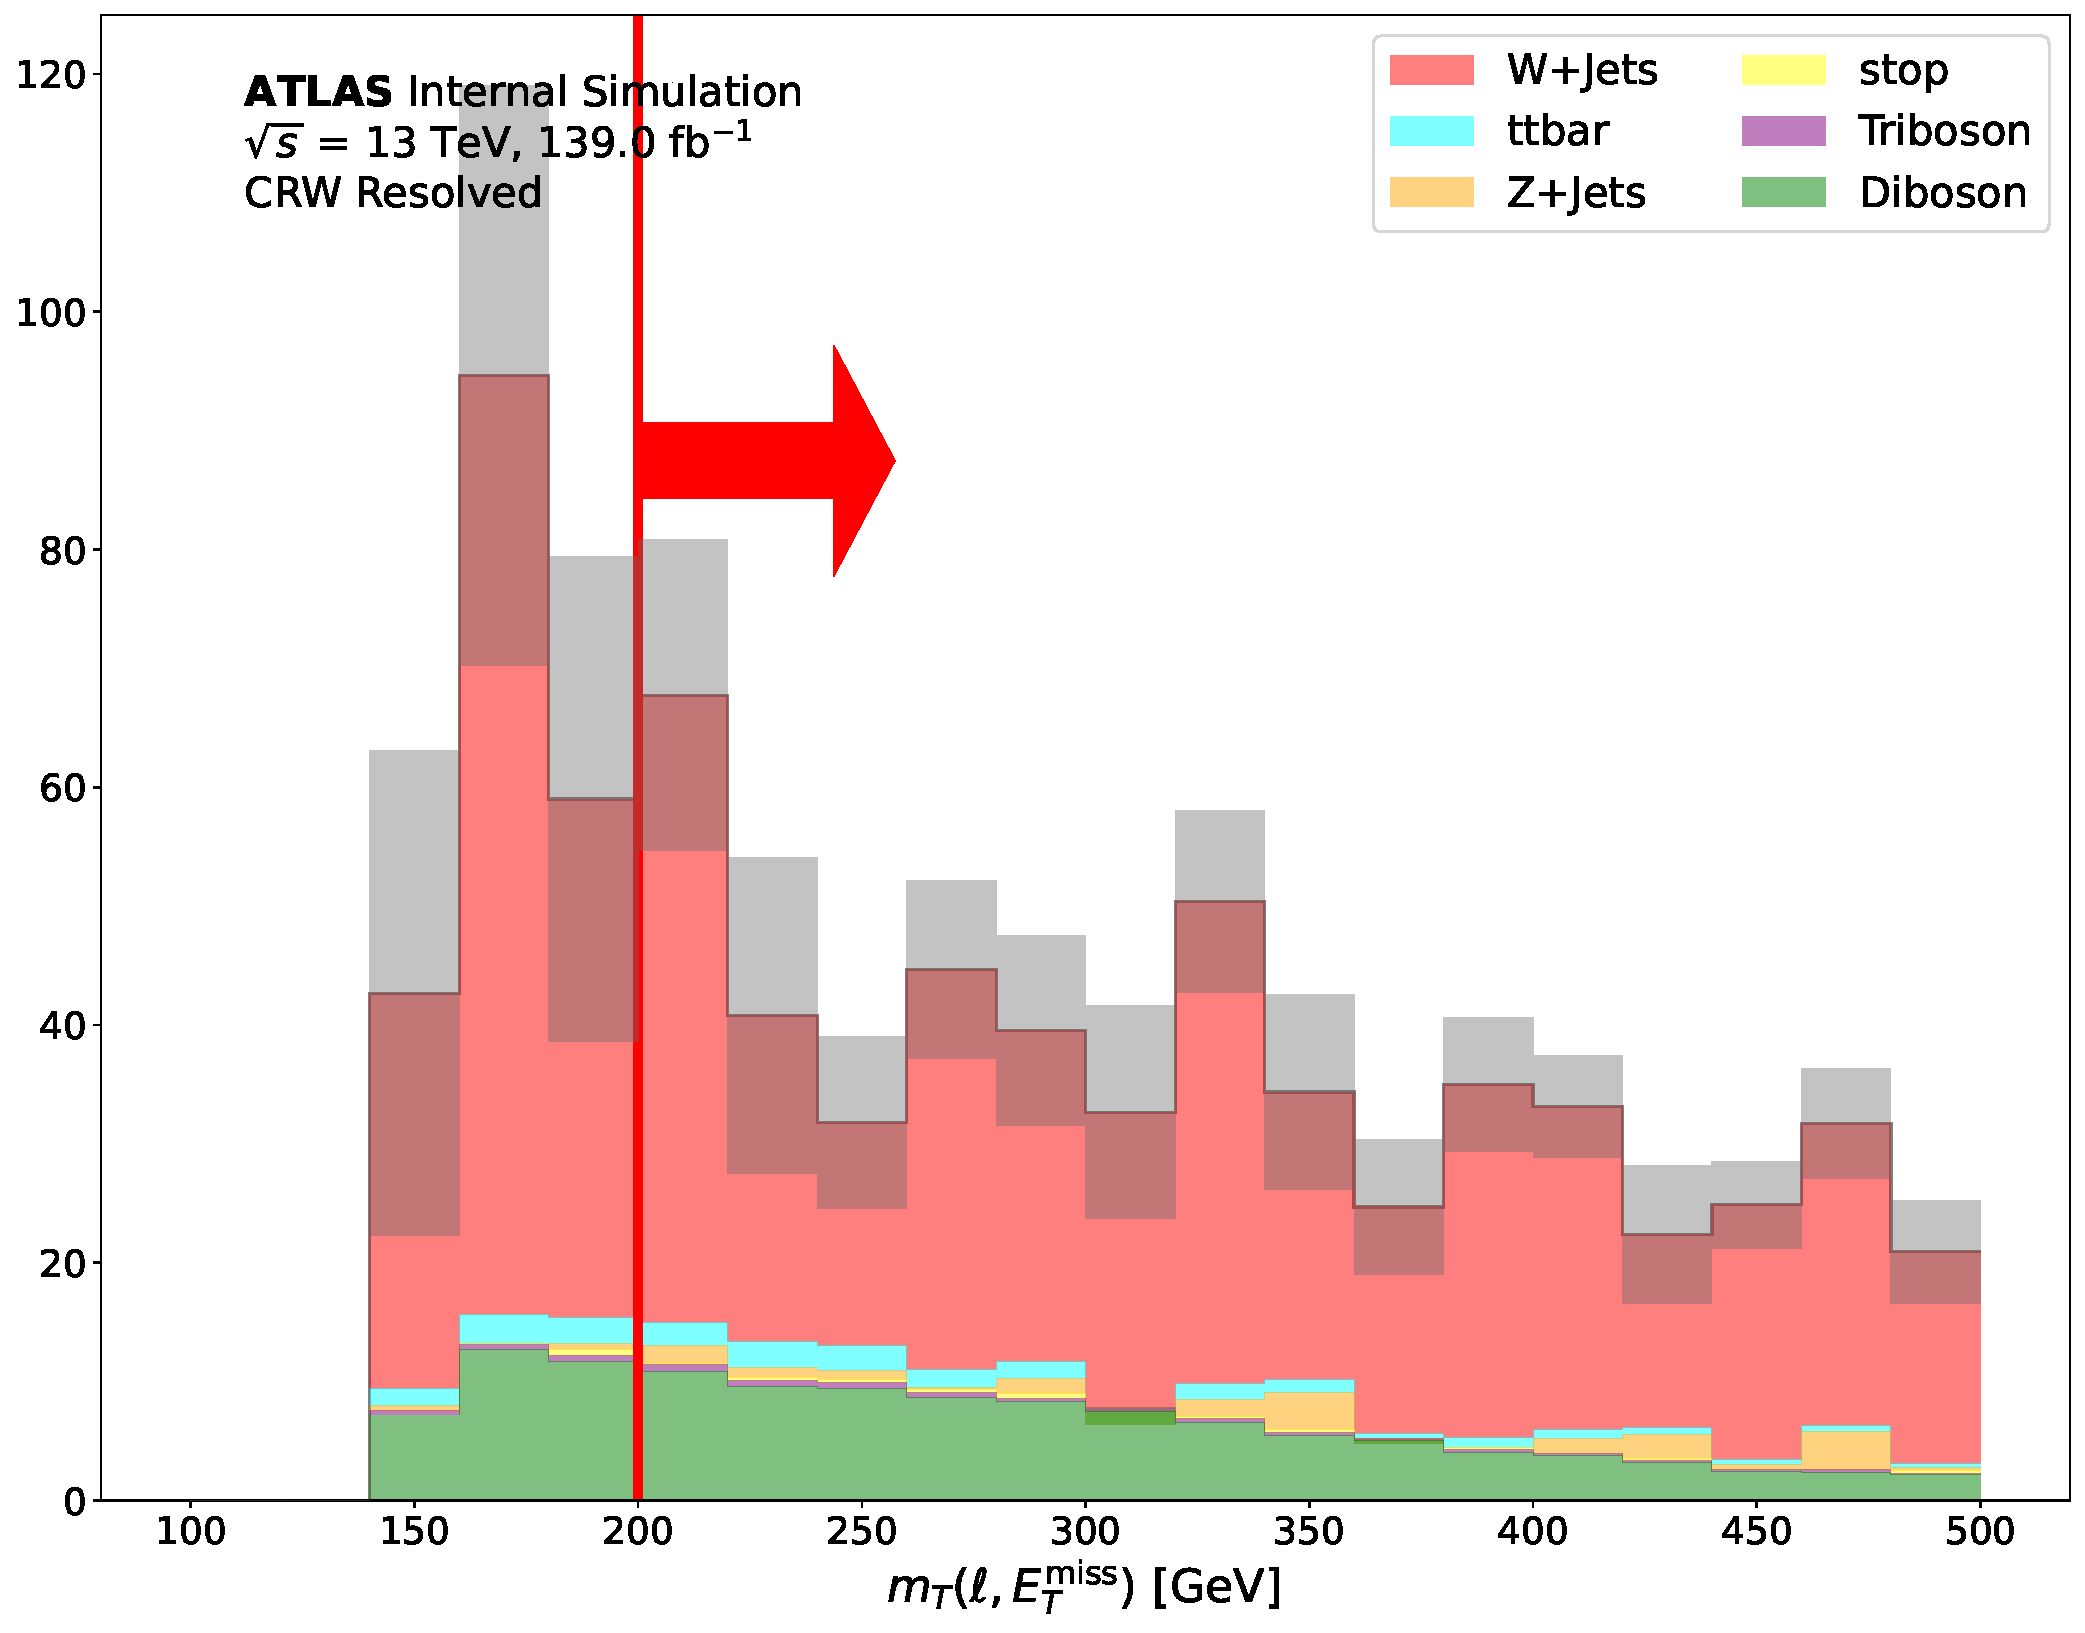
\includegraphics[width = 0.95\textwidth]{Figures/App_SR_CR_distributions/CRW_Resolved/mT_lep_met_N_1.pdf}
     \caption{\mtlepmet (resolved \wjets CR)}
     \end{subfigure}

  \begin{subfigure}{0.45\textwidth}
     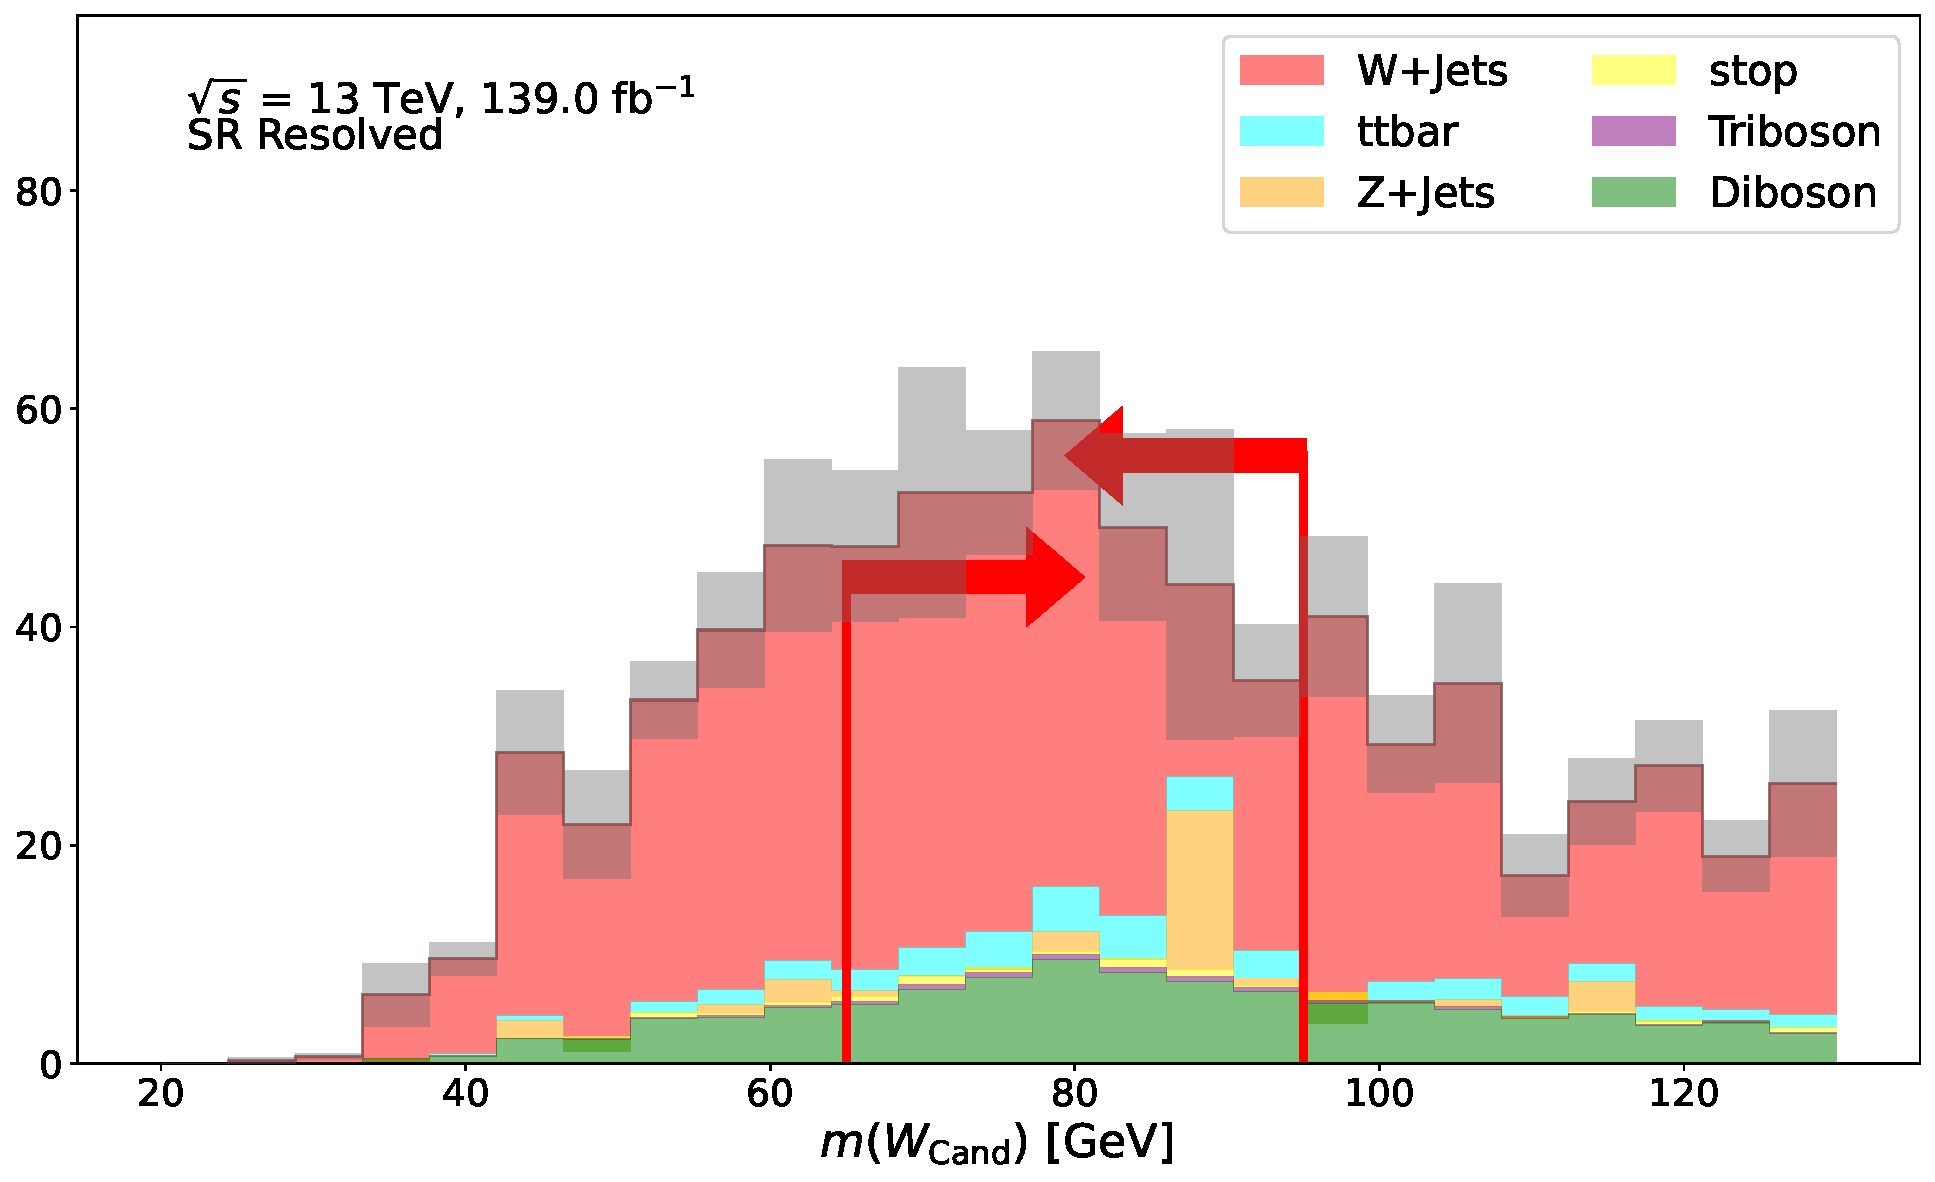
\includegraphics[width = 0.95\textwidth]{Figures/App_SR_CR_distributions/SR1L_Resolved/WCand_m_N_1.pdf}
    \caption{\Wcandm (resolved SR)}
     \end{subfigure}
    \begin{subfigure}{0.45\textwidth}
     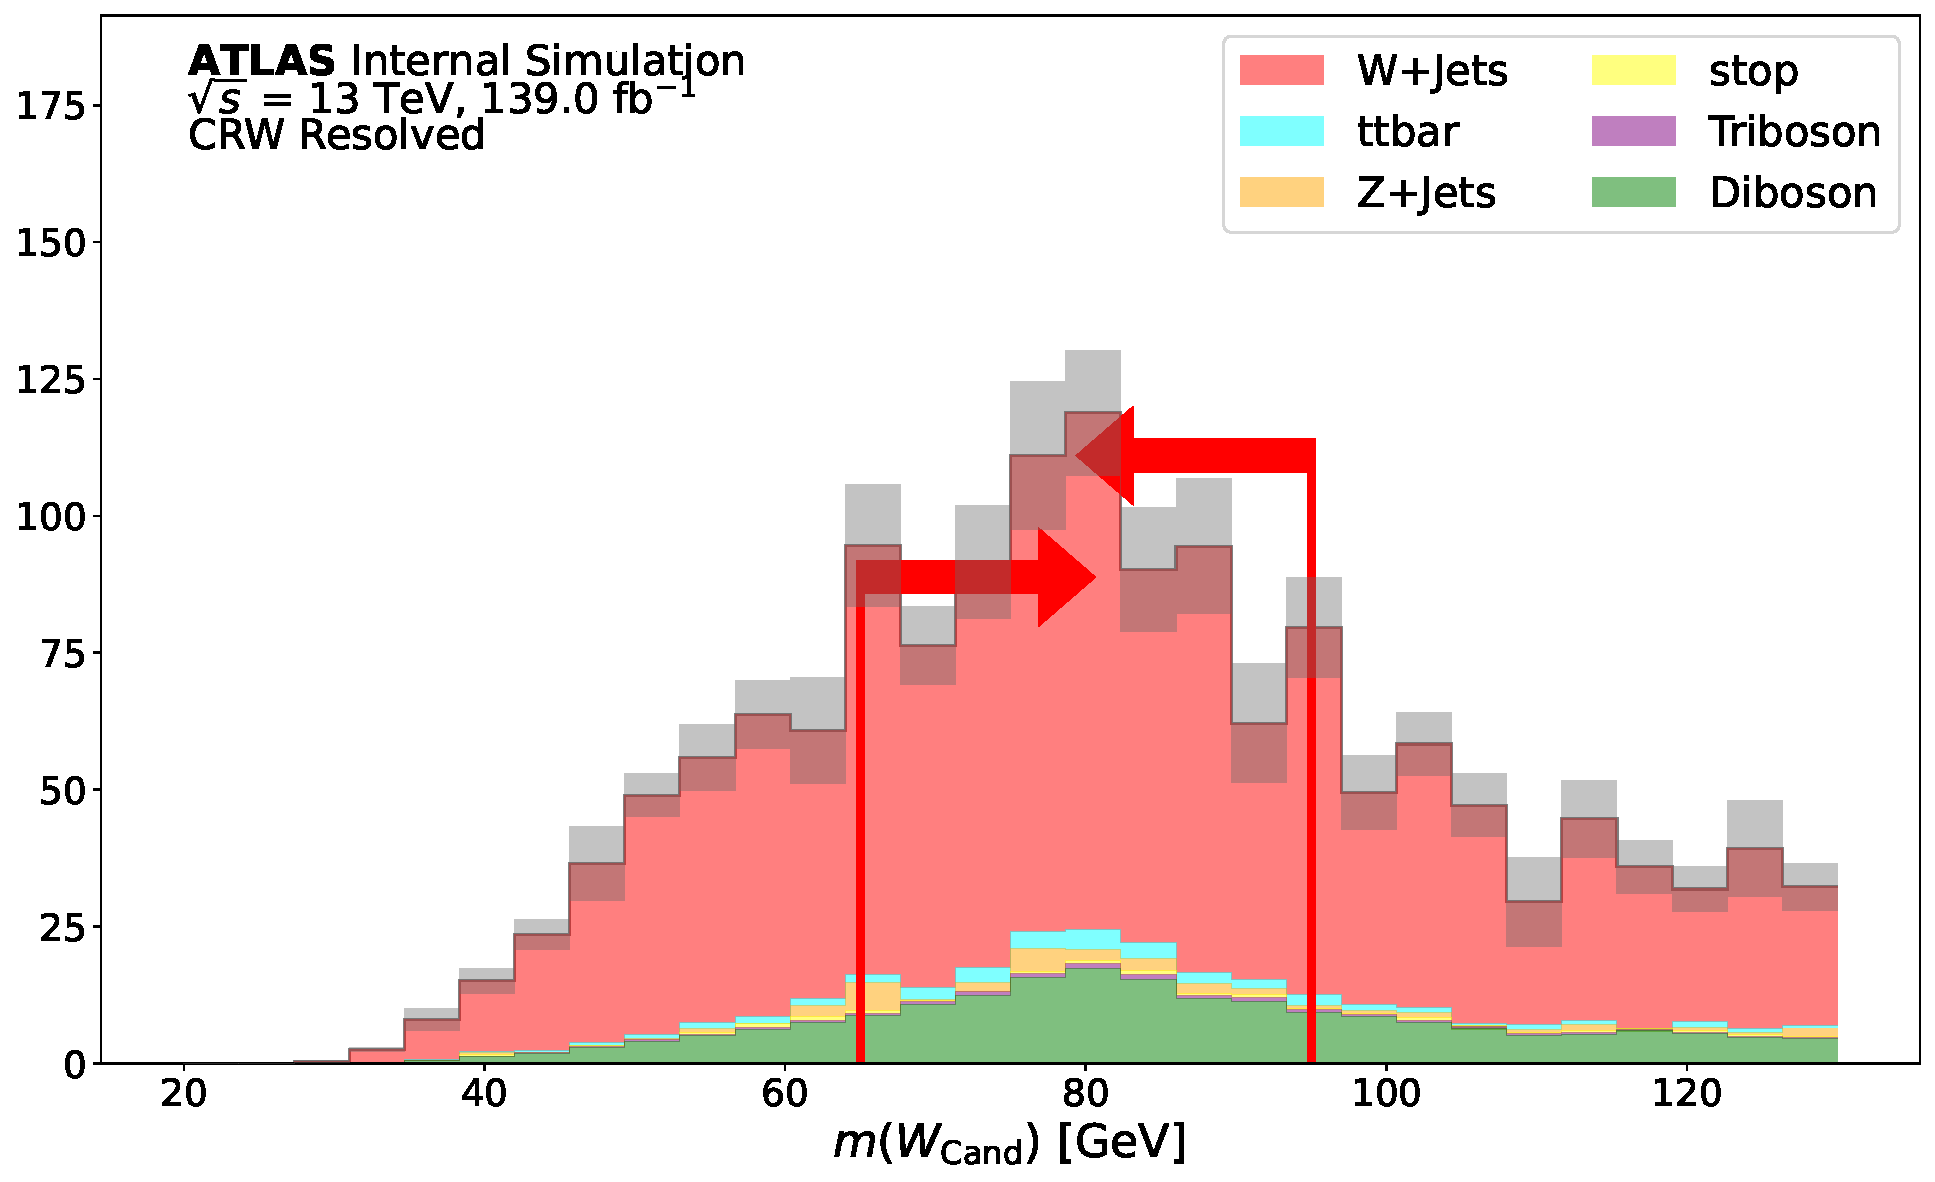
\includegraphics[width = 0.95\textwidth]{Figures/App_SR_CR_distributions/CRW_Resolved/WCand_m_N_1.pdf}
     \caption{\Wcandm (resolved \wjets CR)}
     \end{subfigure}

  \begin{subfigure}{0.45\textwidth}
     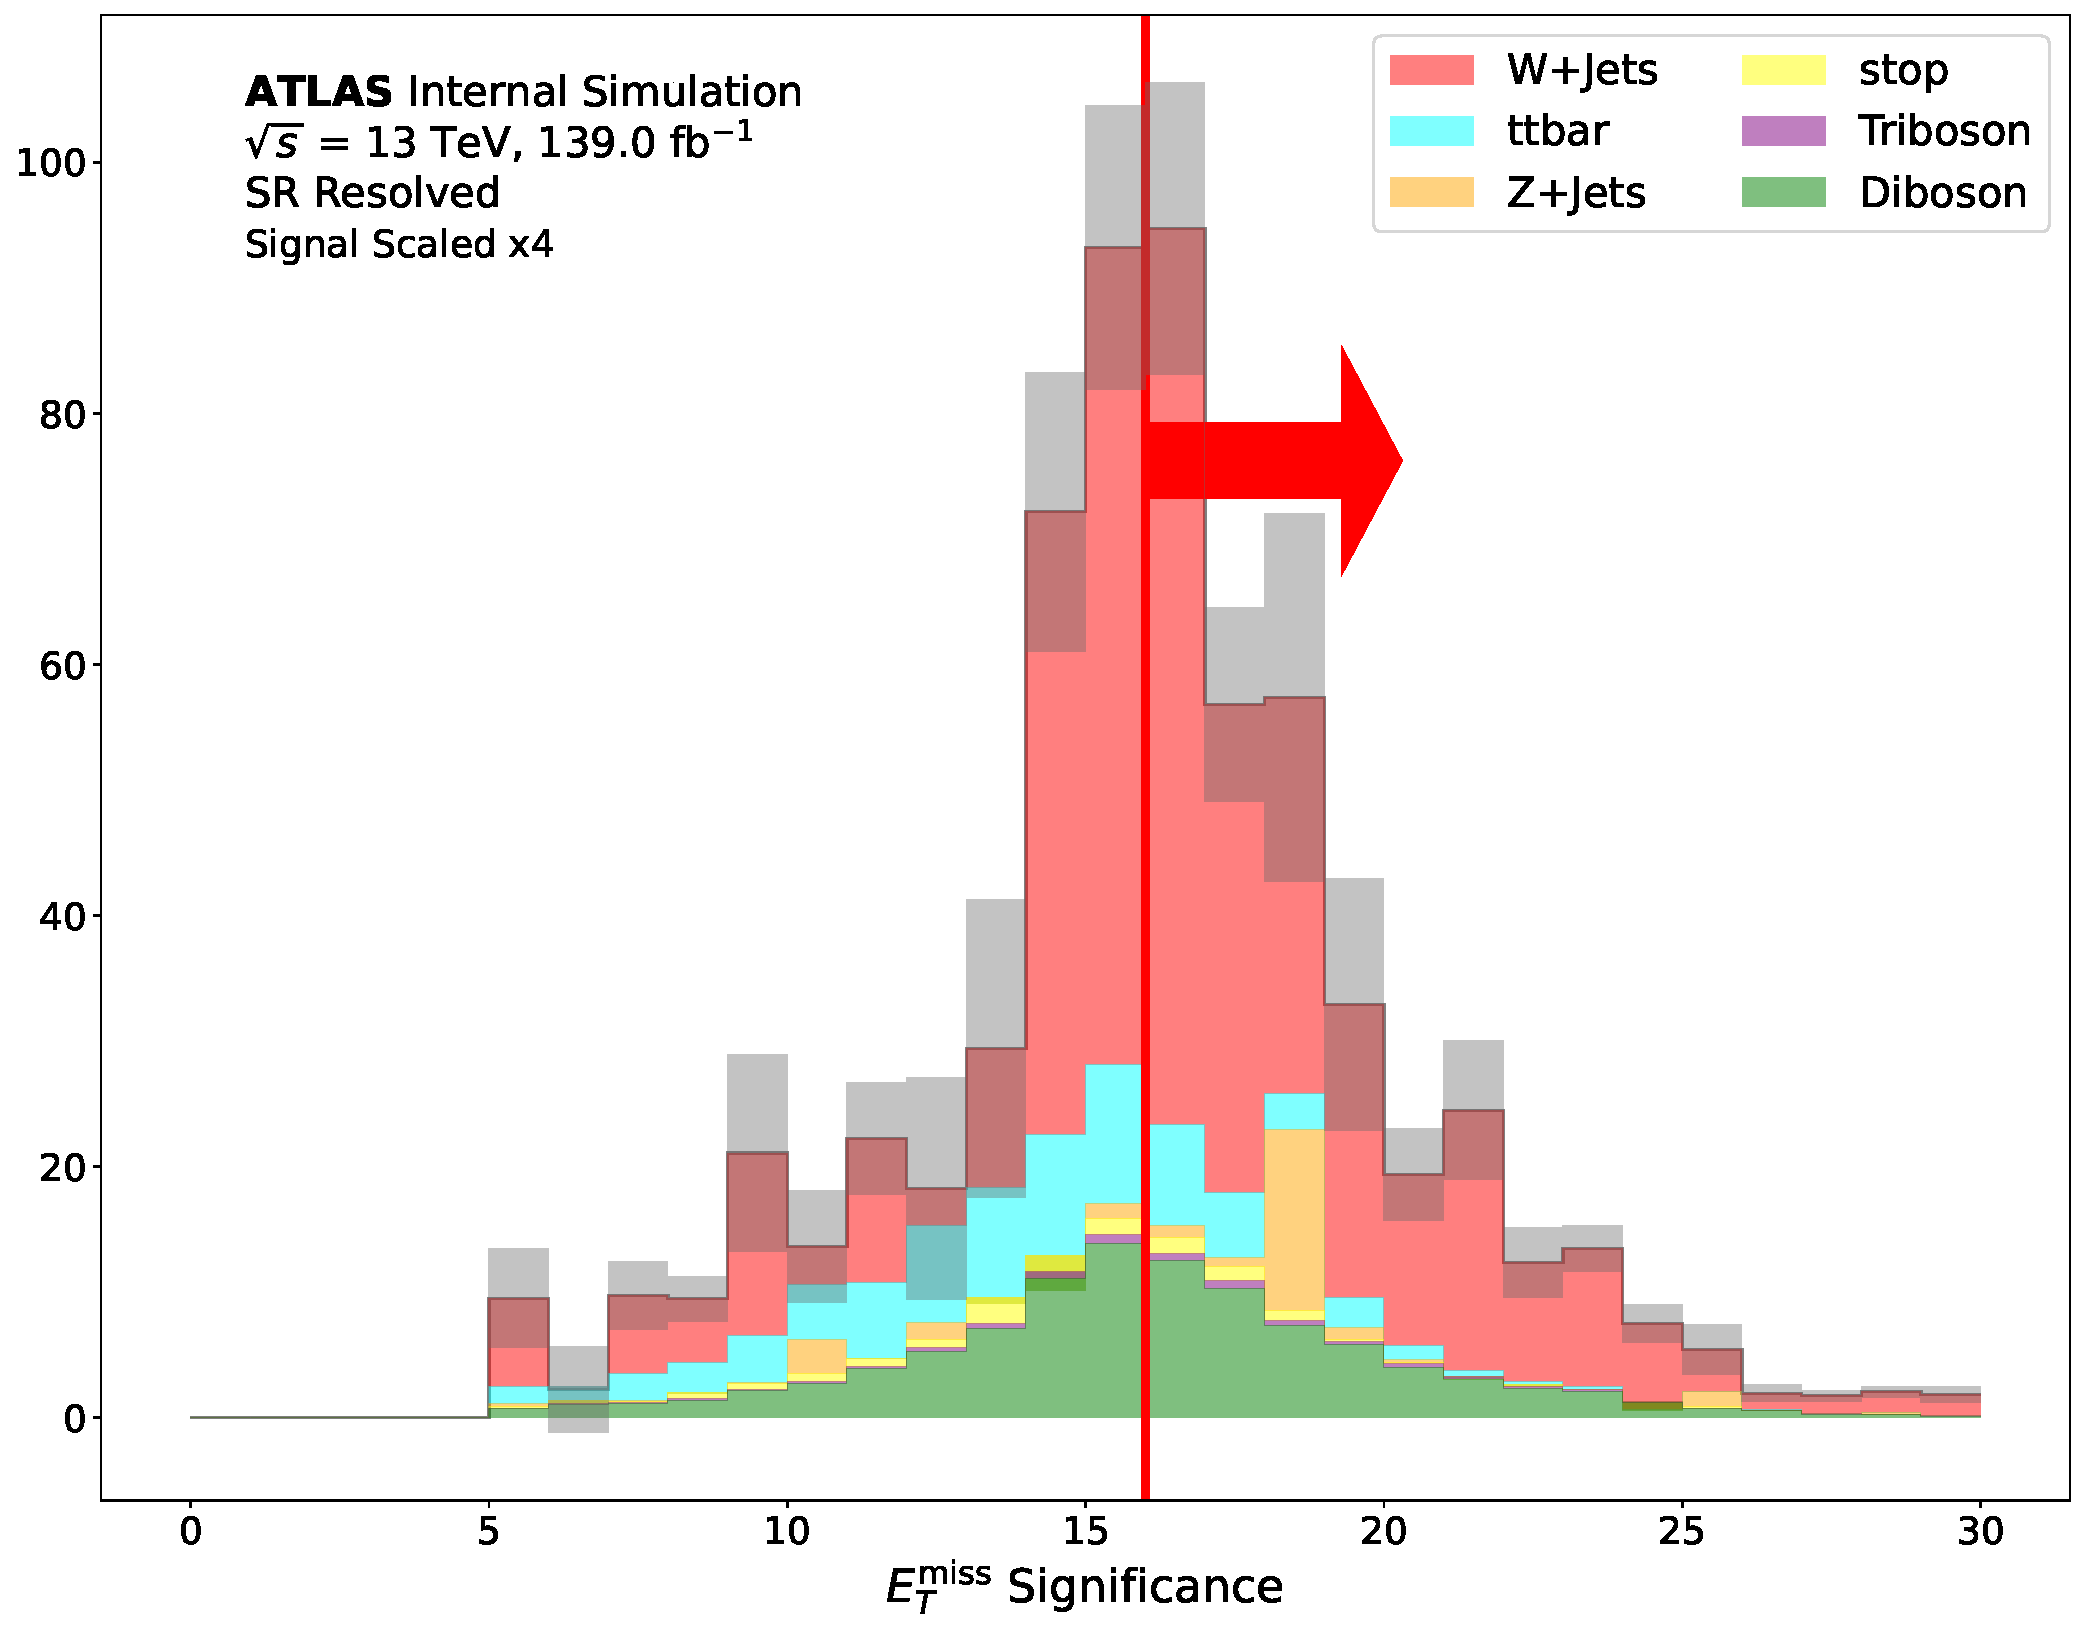
\includegraphics[width = 0.95\textwidth]{Figures/App_SR_CR_distributions/SR1L_Resolved/MetTST_Significance_N_1.pdf}
    \caption{\metsig (resolved SR)}
     \end{subfigure}
    \begin{subfigure}{0.45\textwidth}
     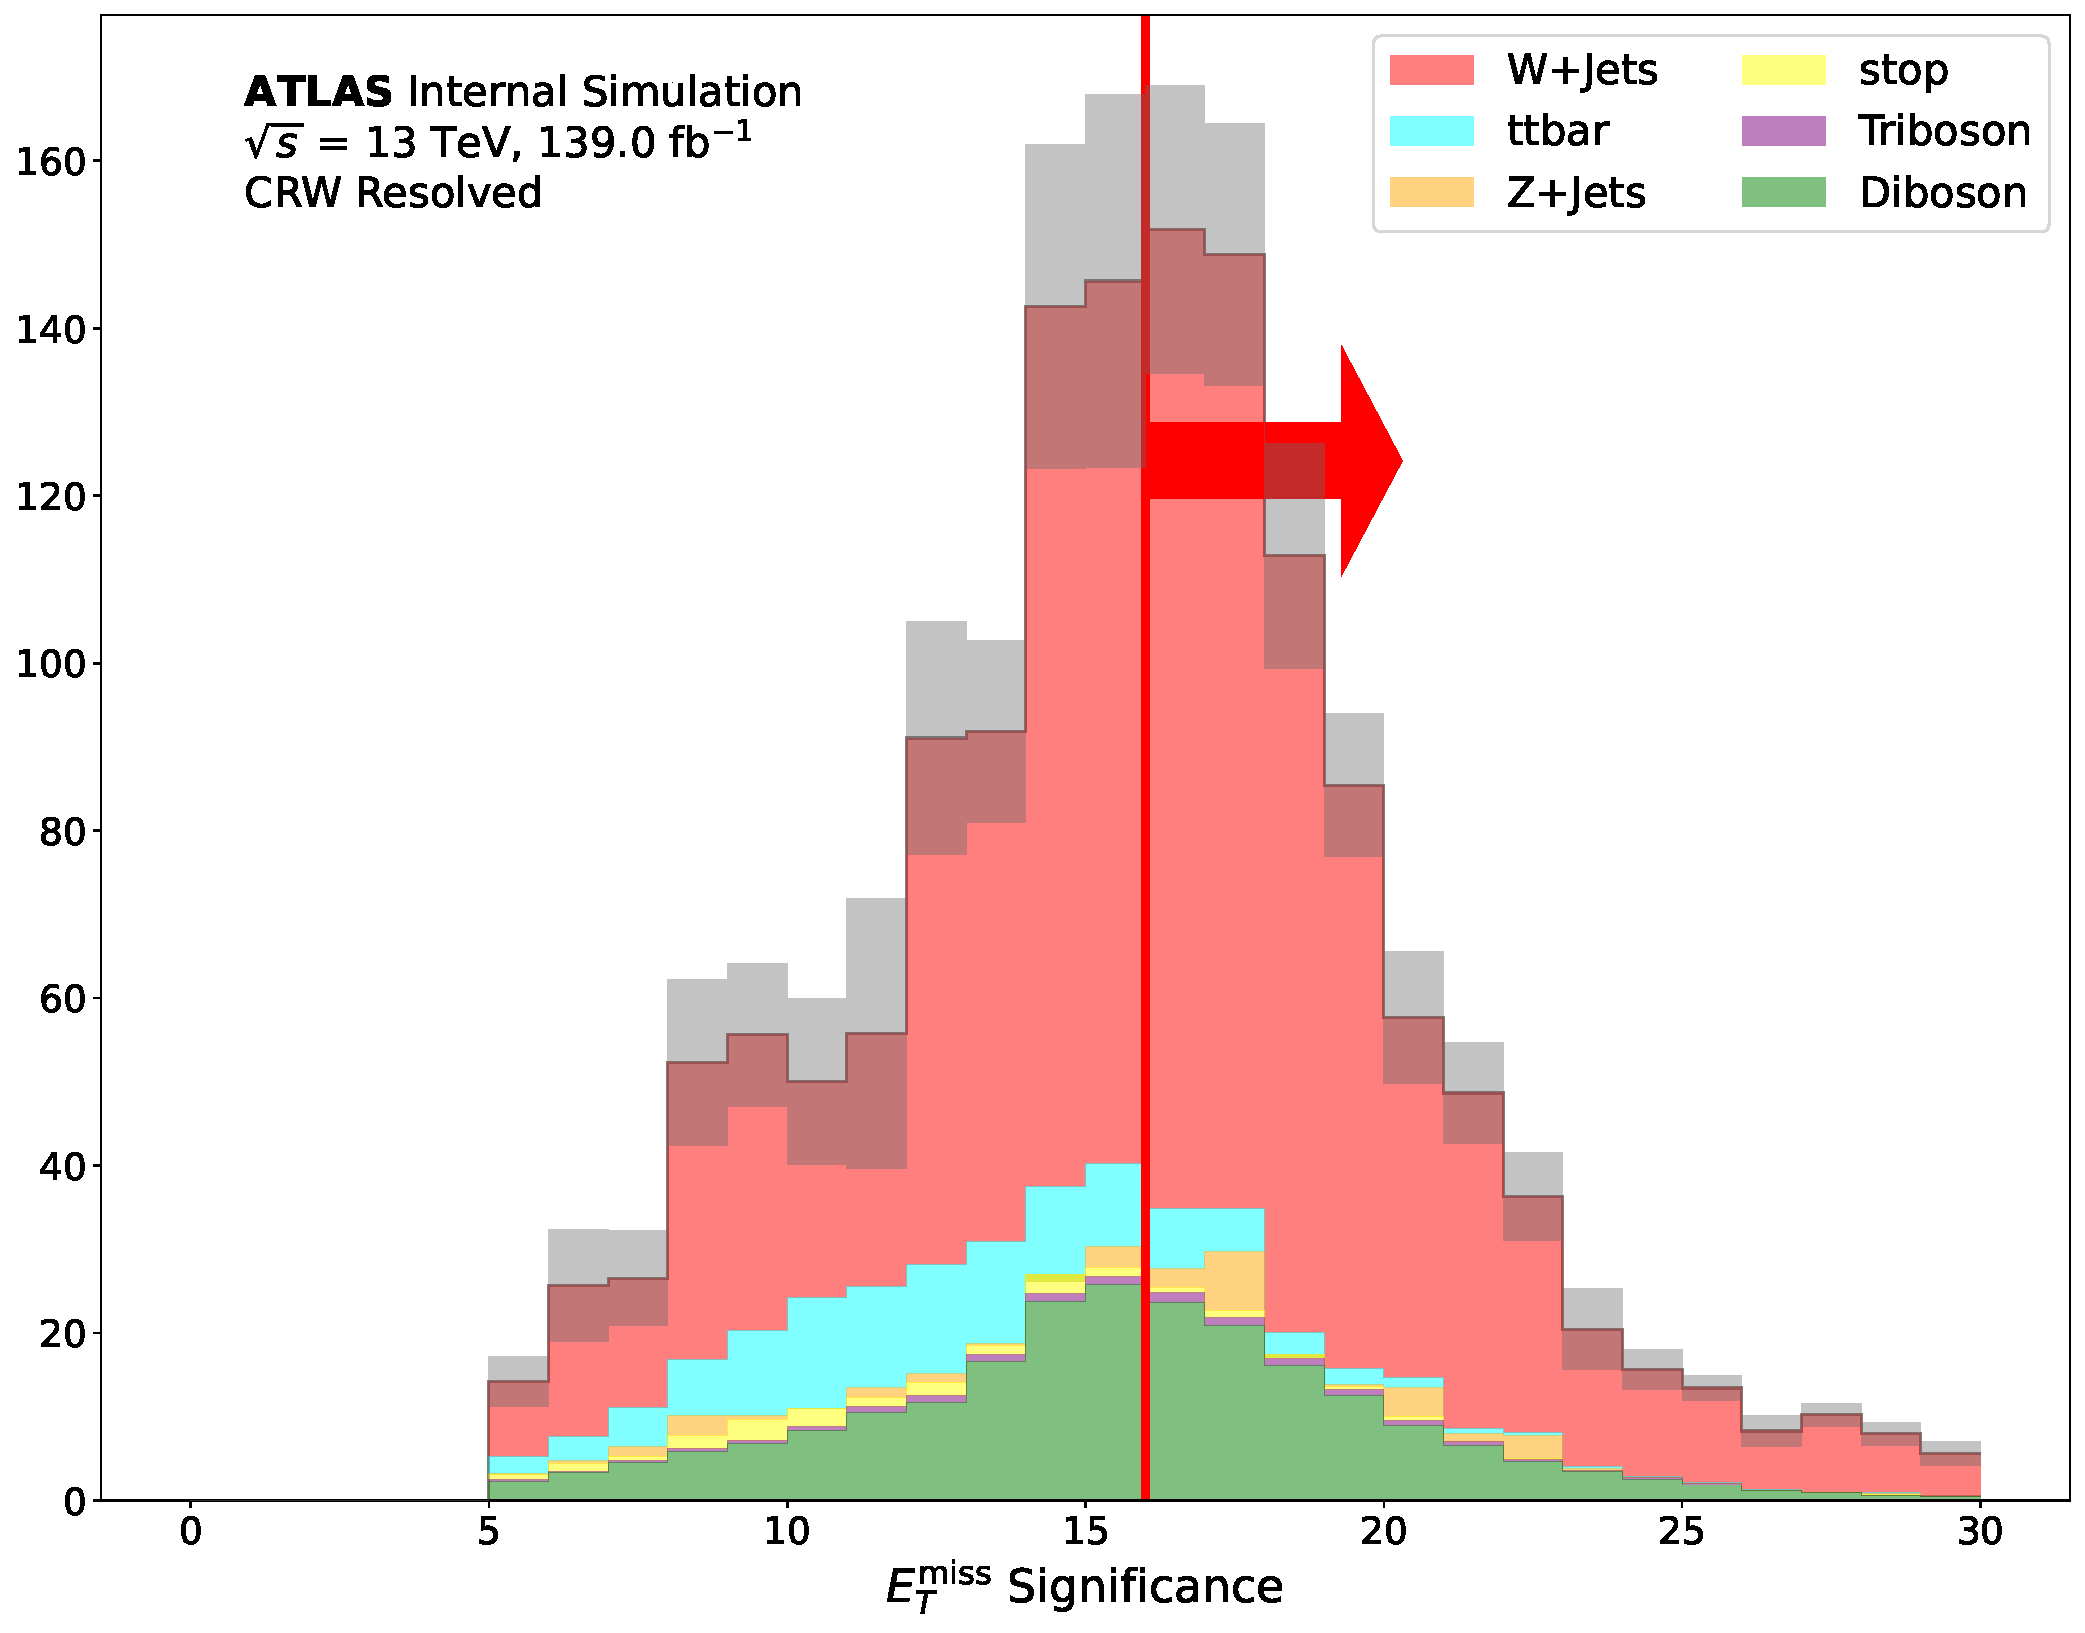
\includegraphics[width = 0.95\textwidth]{Figures/App_SR_CR_distributions/CRW_Resolved/MetTST_Significance_N_1.pdf}
     \caption{\metsig (resolved \wjets CR)}
     \end{subfigure}
      \caption{Comparison of N-1 distributions for kinematic variables of interest between the SR and the \wjets CR in the resolved category. Grey bands show statistical uncertainty on the background estimate.}
     \label{fig:N_1_CRW_resolved}    
     \end{figure}
     \begin{figure}[htbp] \ContinuedFloat
    \begin{subfigure}{0.45\textwidth}
     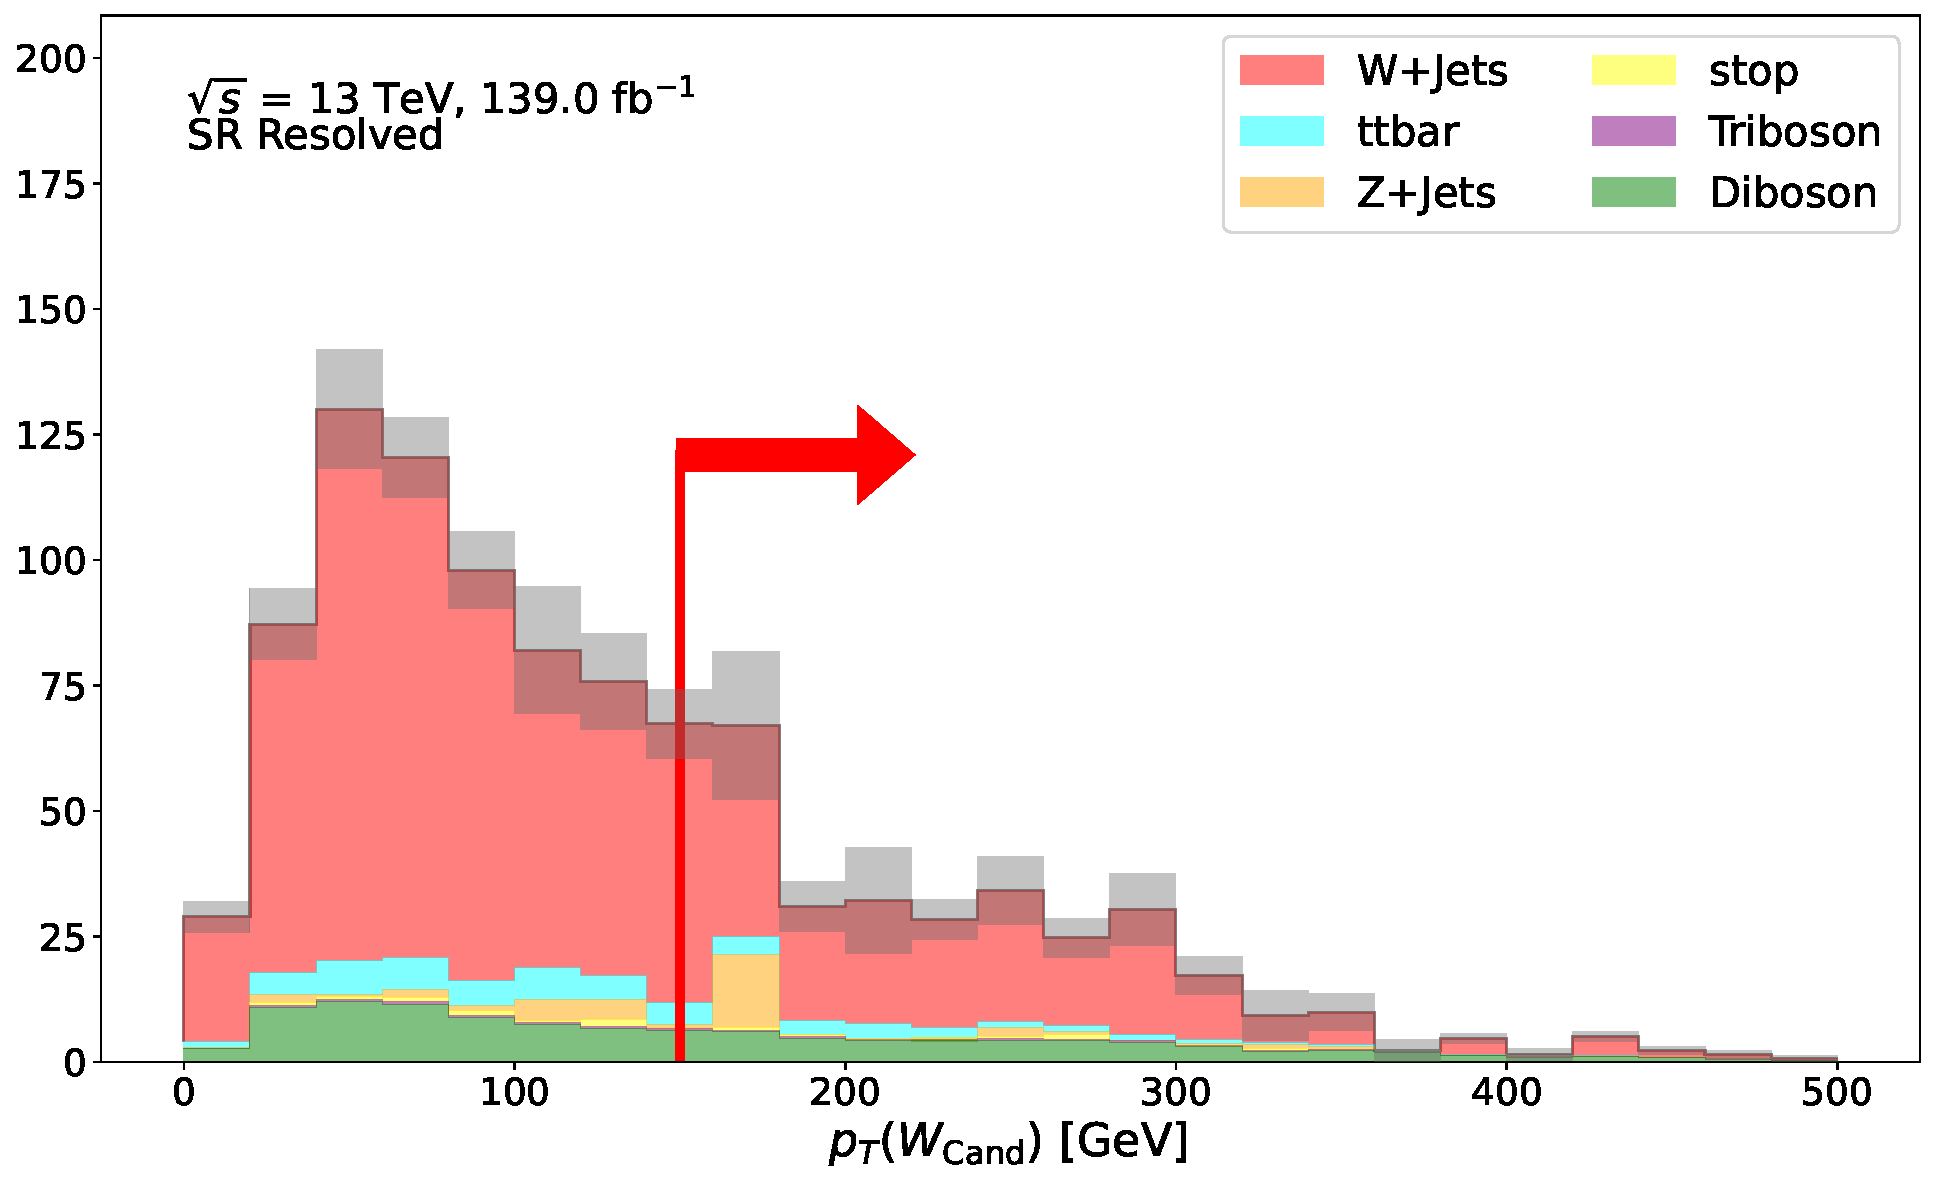
\includegraphics[width = 0.95\textwidth]{Figures/App_SR_CR_distributions/SR1L_Resolved/WCand_pt_N_1.pdf}
    \caption{\Wcandpt (resolved SR)}
     \end{subfigure}
    \begin{subfigure}{0.45\textwidth}
     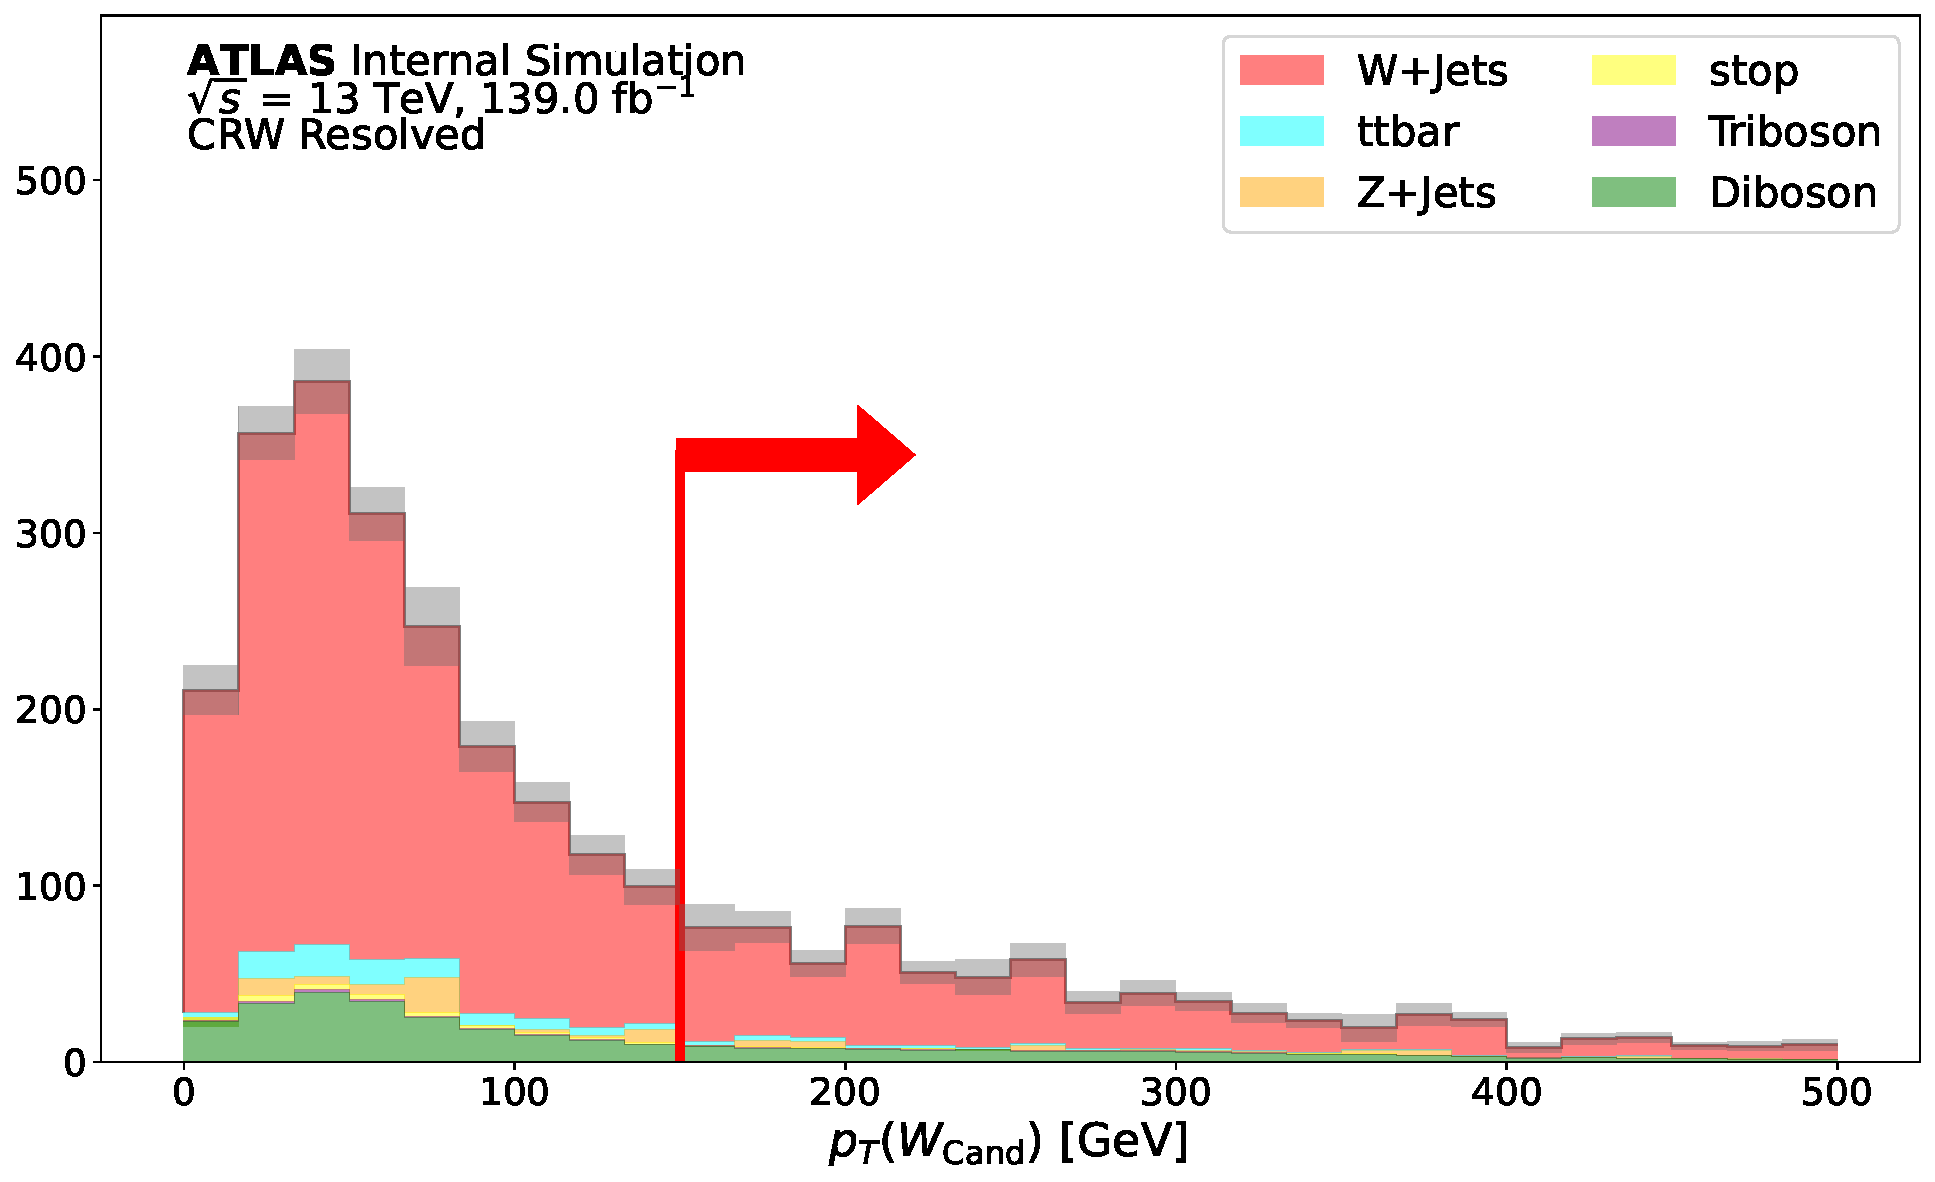
\includegraphics[width = 0.95\textwidth]{Figures/App_SR_CR_distributions/CRW_Resolved/WCand_pt_N_1.pdf}
     \caption{\Wcandpt (resolved \wjets CR)}
     \end{subfigure}   
    \begin{subfigure}{0.45\textwidth}
     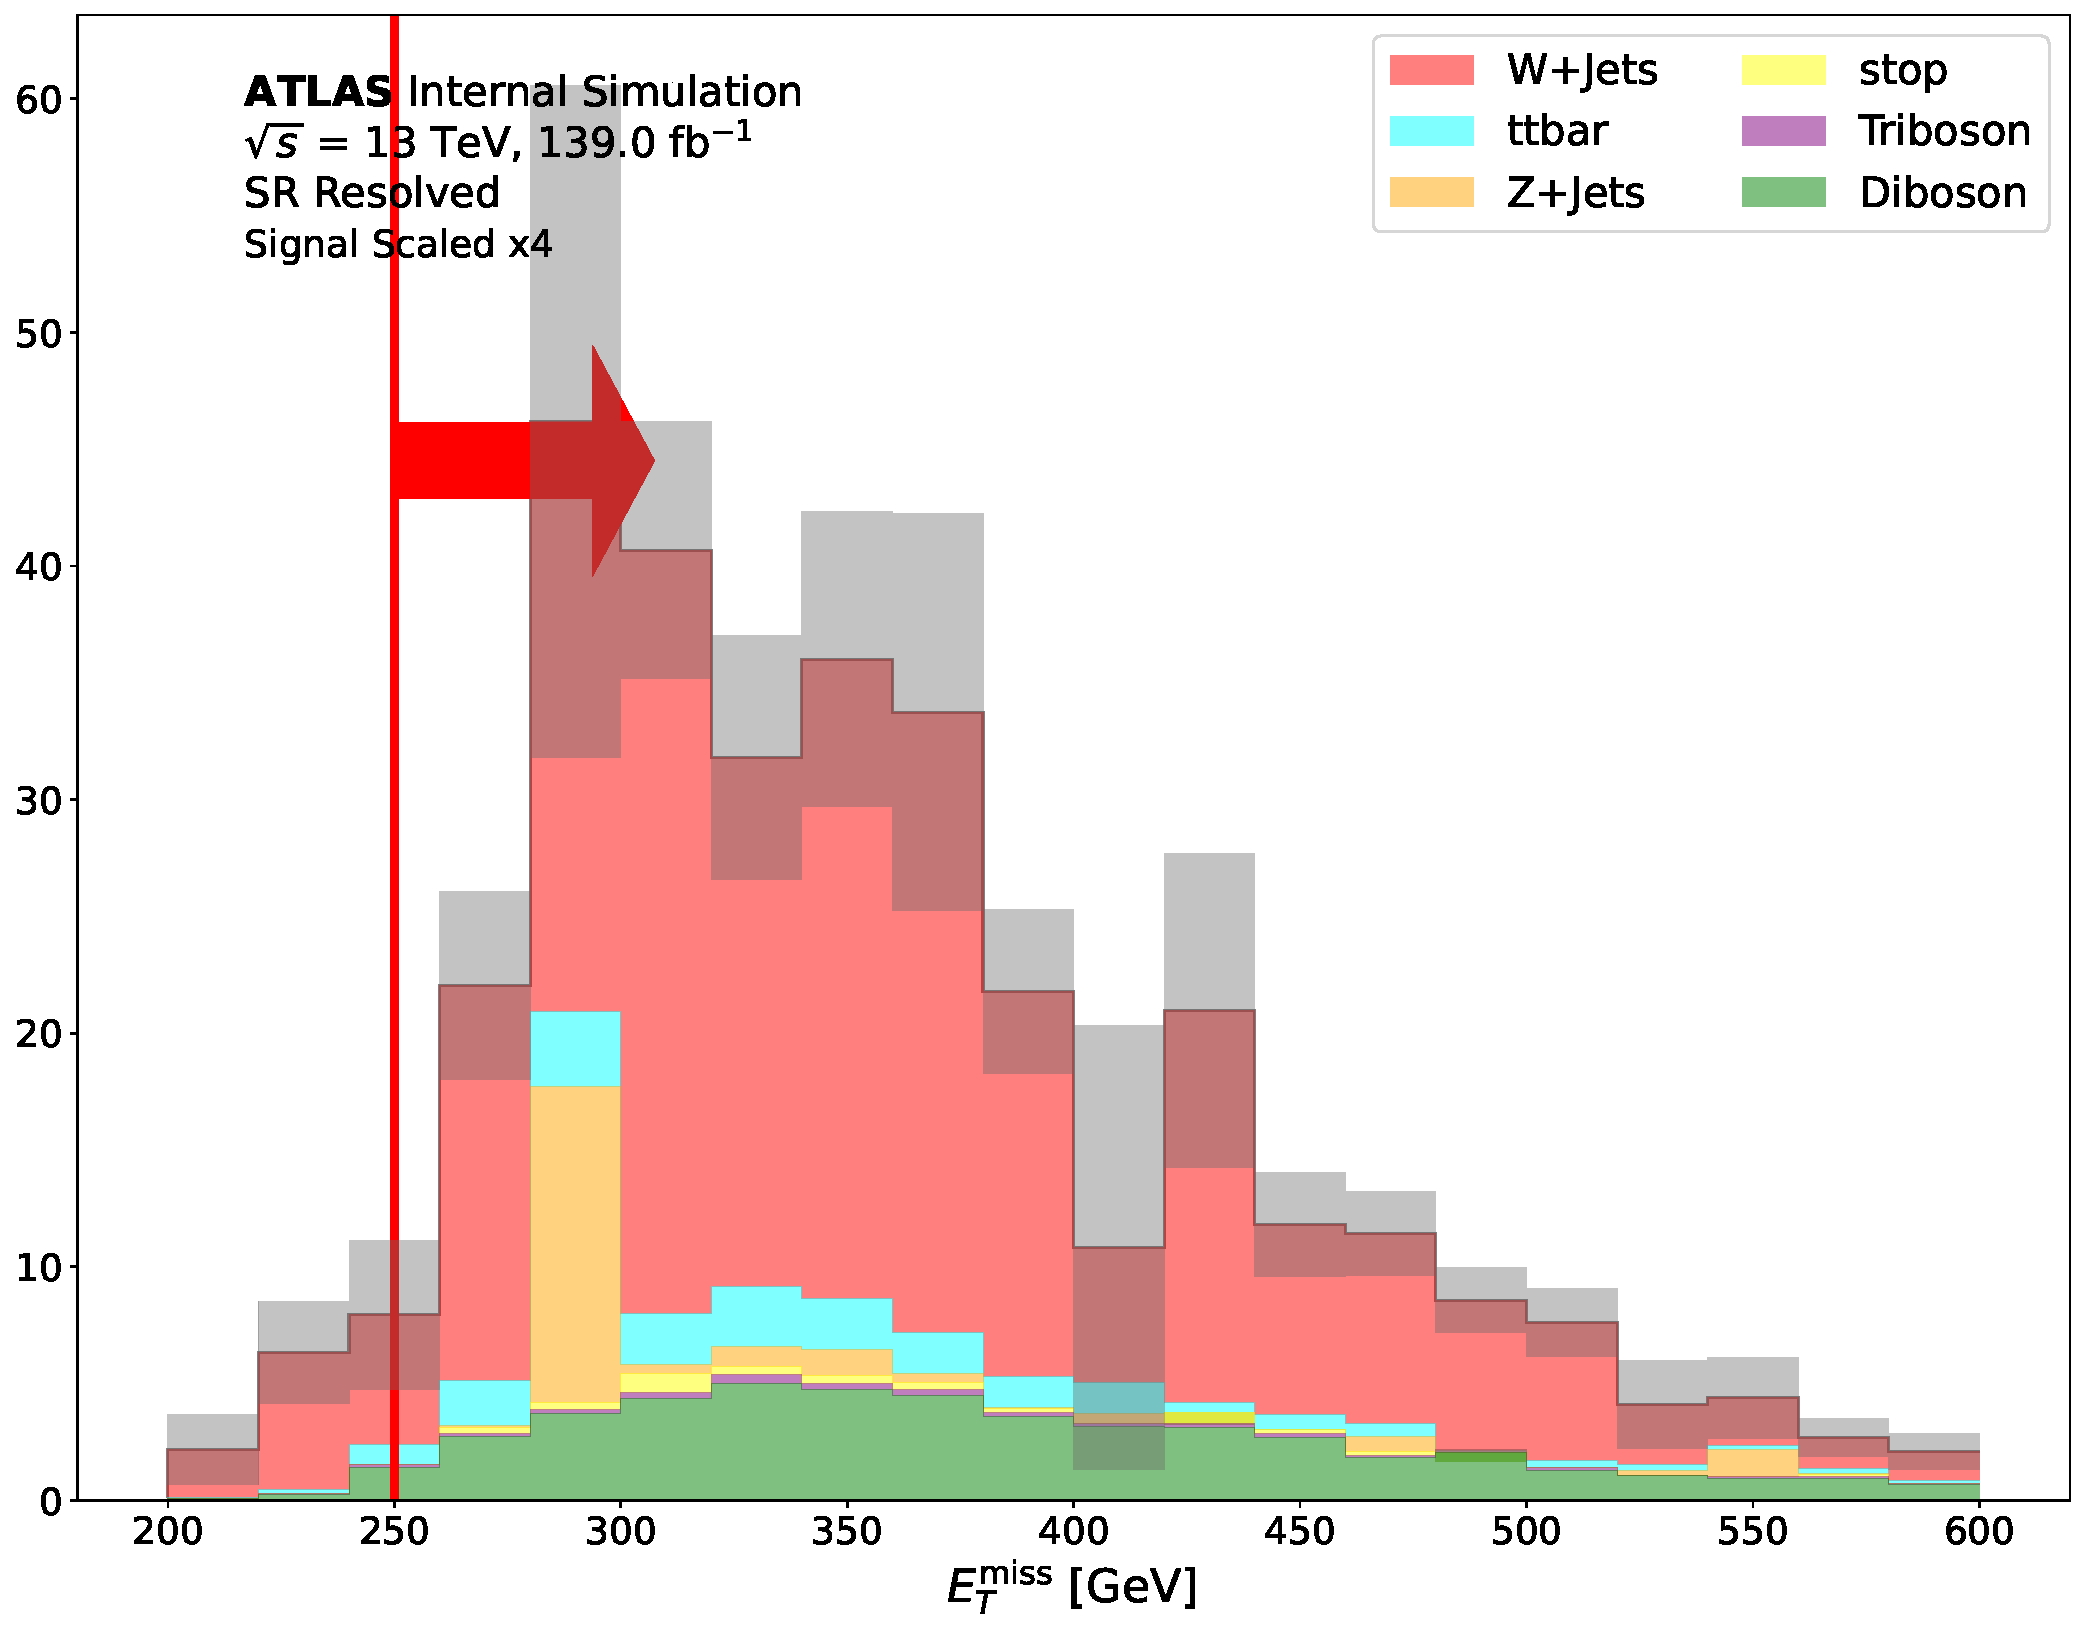
\includegraphics[width = 0.95\textwidth]{Figures/App_SR_CR_distributions/SR1L_Resolved/MetTST_met_N_1.pdf}
    \caption{\met (resolved SR)}
     \end{subfigure}
    \begin{subfigure}{0.45\textwidth}
     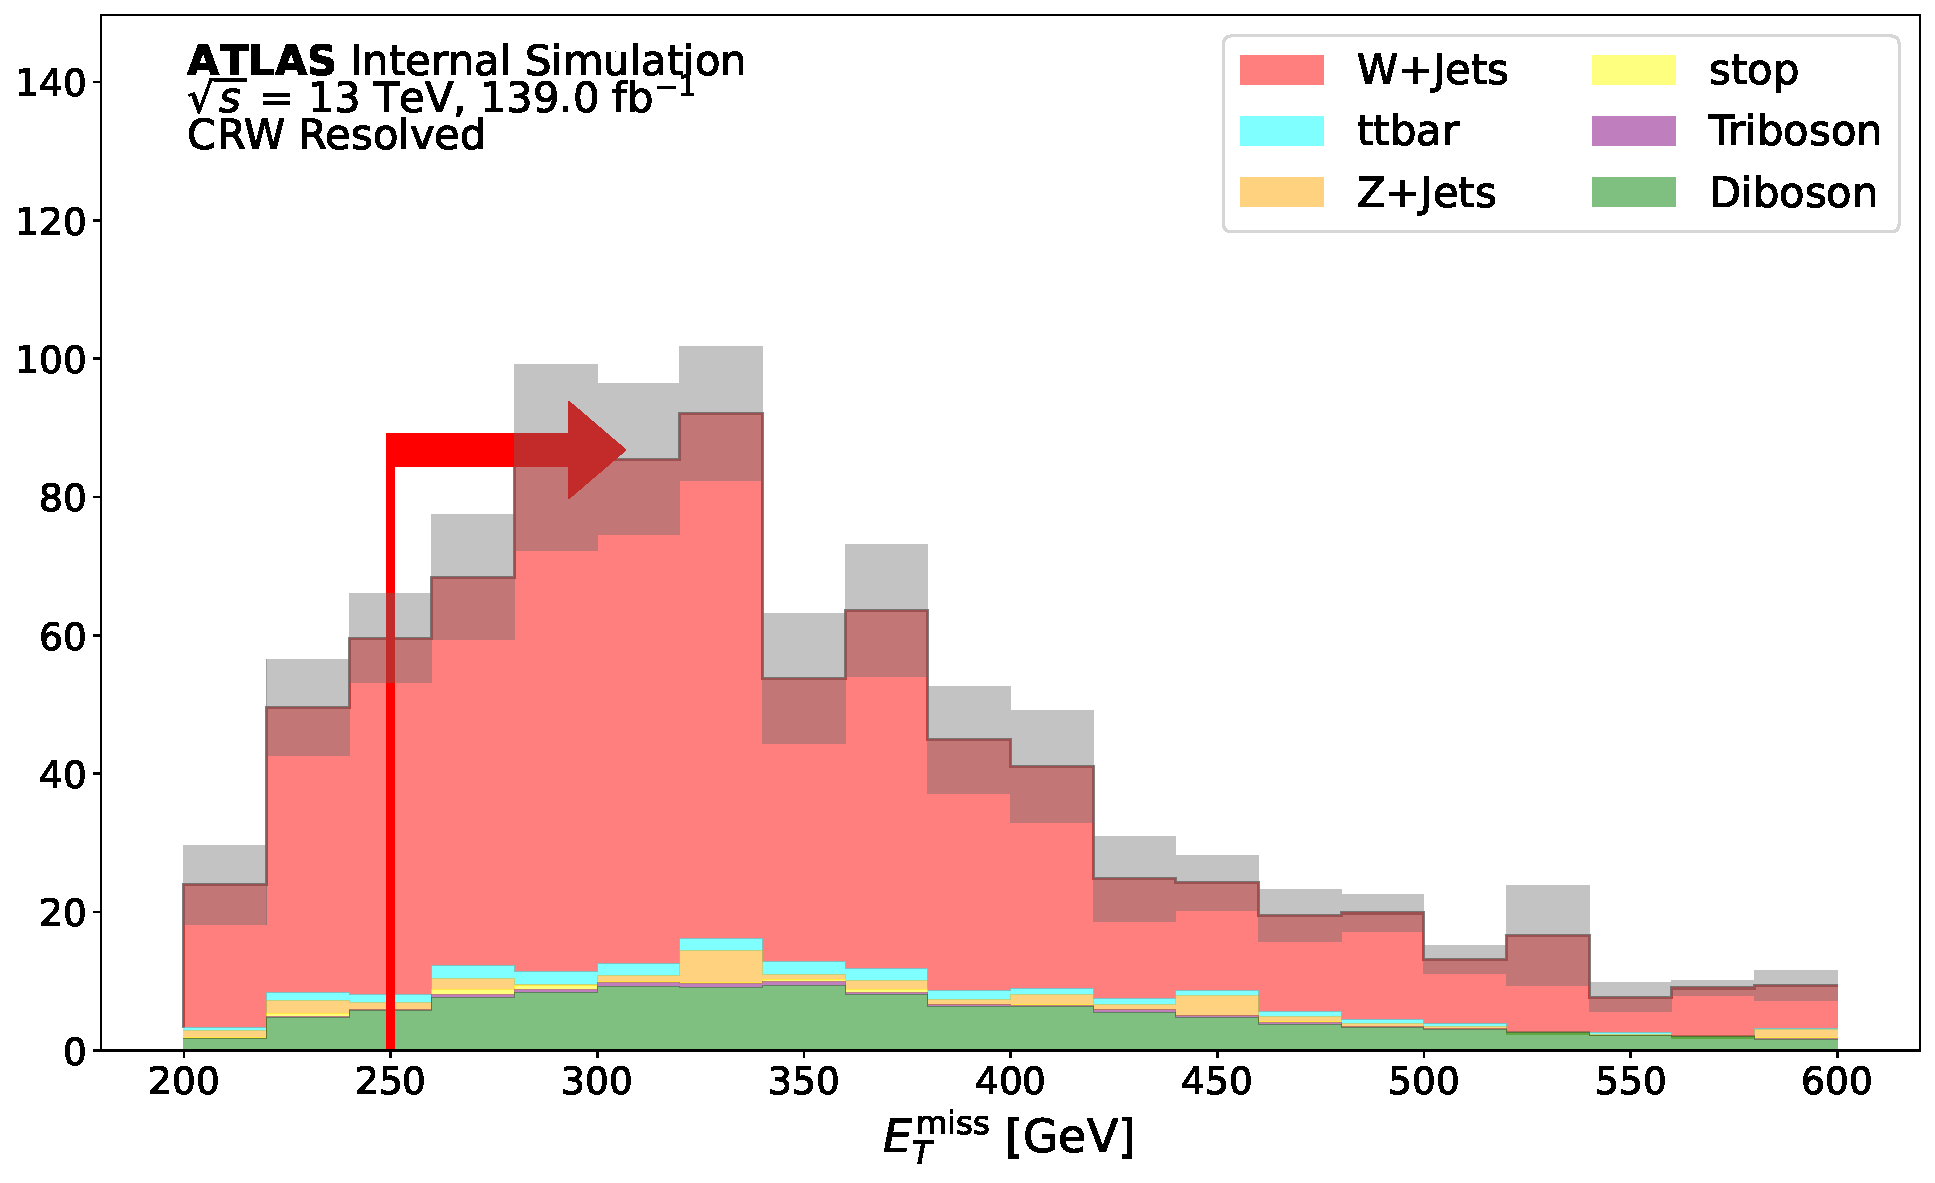
\includegraphics[width = 0.95\textwidth]{Figures/App_SR_CR_distributions/CRW_Resolved/MetTST_met_N_1.pdf}
     \caption{\met (resolved \wjets CR)}
     \end{subfigure}
     \caption{Comparison of N-1 distributions for kinematic variables of interest between the SR and the \wjets CR in the resolved category (continued).}
  \end{figure}


\section{Signal region vs. \ttbar control region}
\label{app:appendix_SR_CR_distributions_ttbar}

\Fig{~\ref{fig:N_1_CRTT_merged}} compares distributions of kinematic variables of interest for the analysis between the merged SR and the \ttbar CR. \Fig{~\ref{fig:N_1_CRTT_resolved}} presents the same comparisons between the resolved SR and the \ttbar CR.

\begin{figure}[htbp]
  \centering
     \begin{subfigure}{0.45\textwidth}
     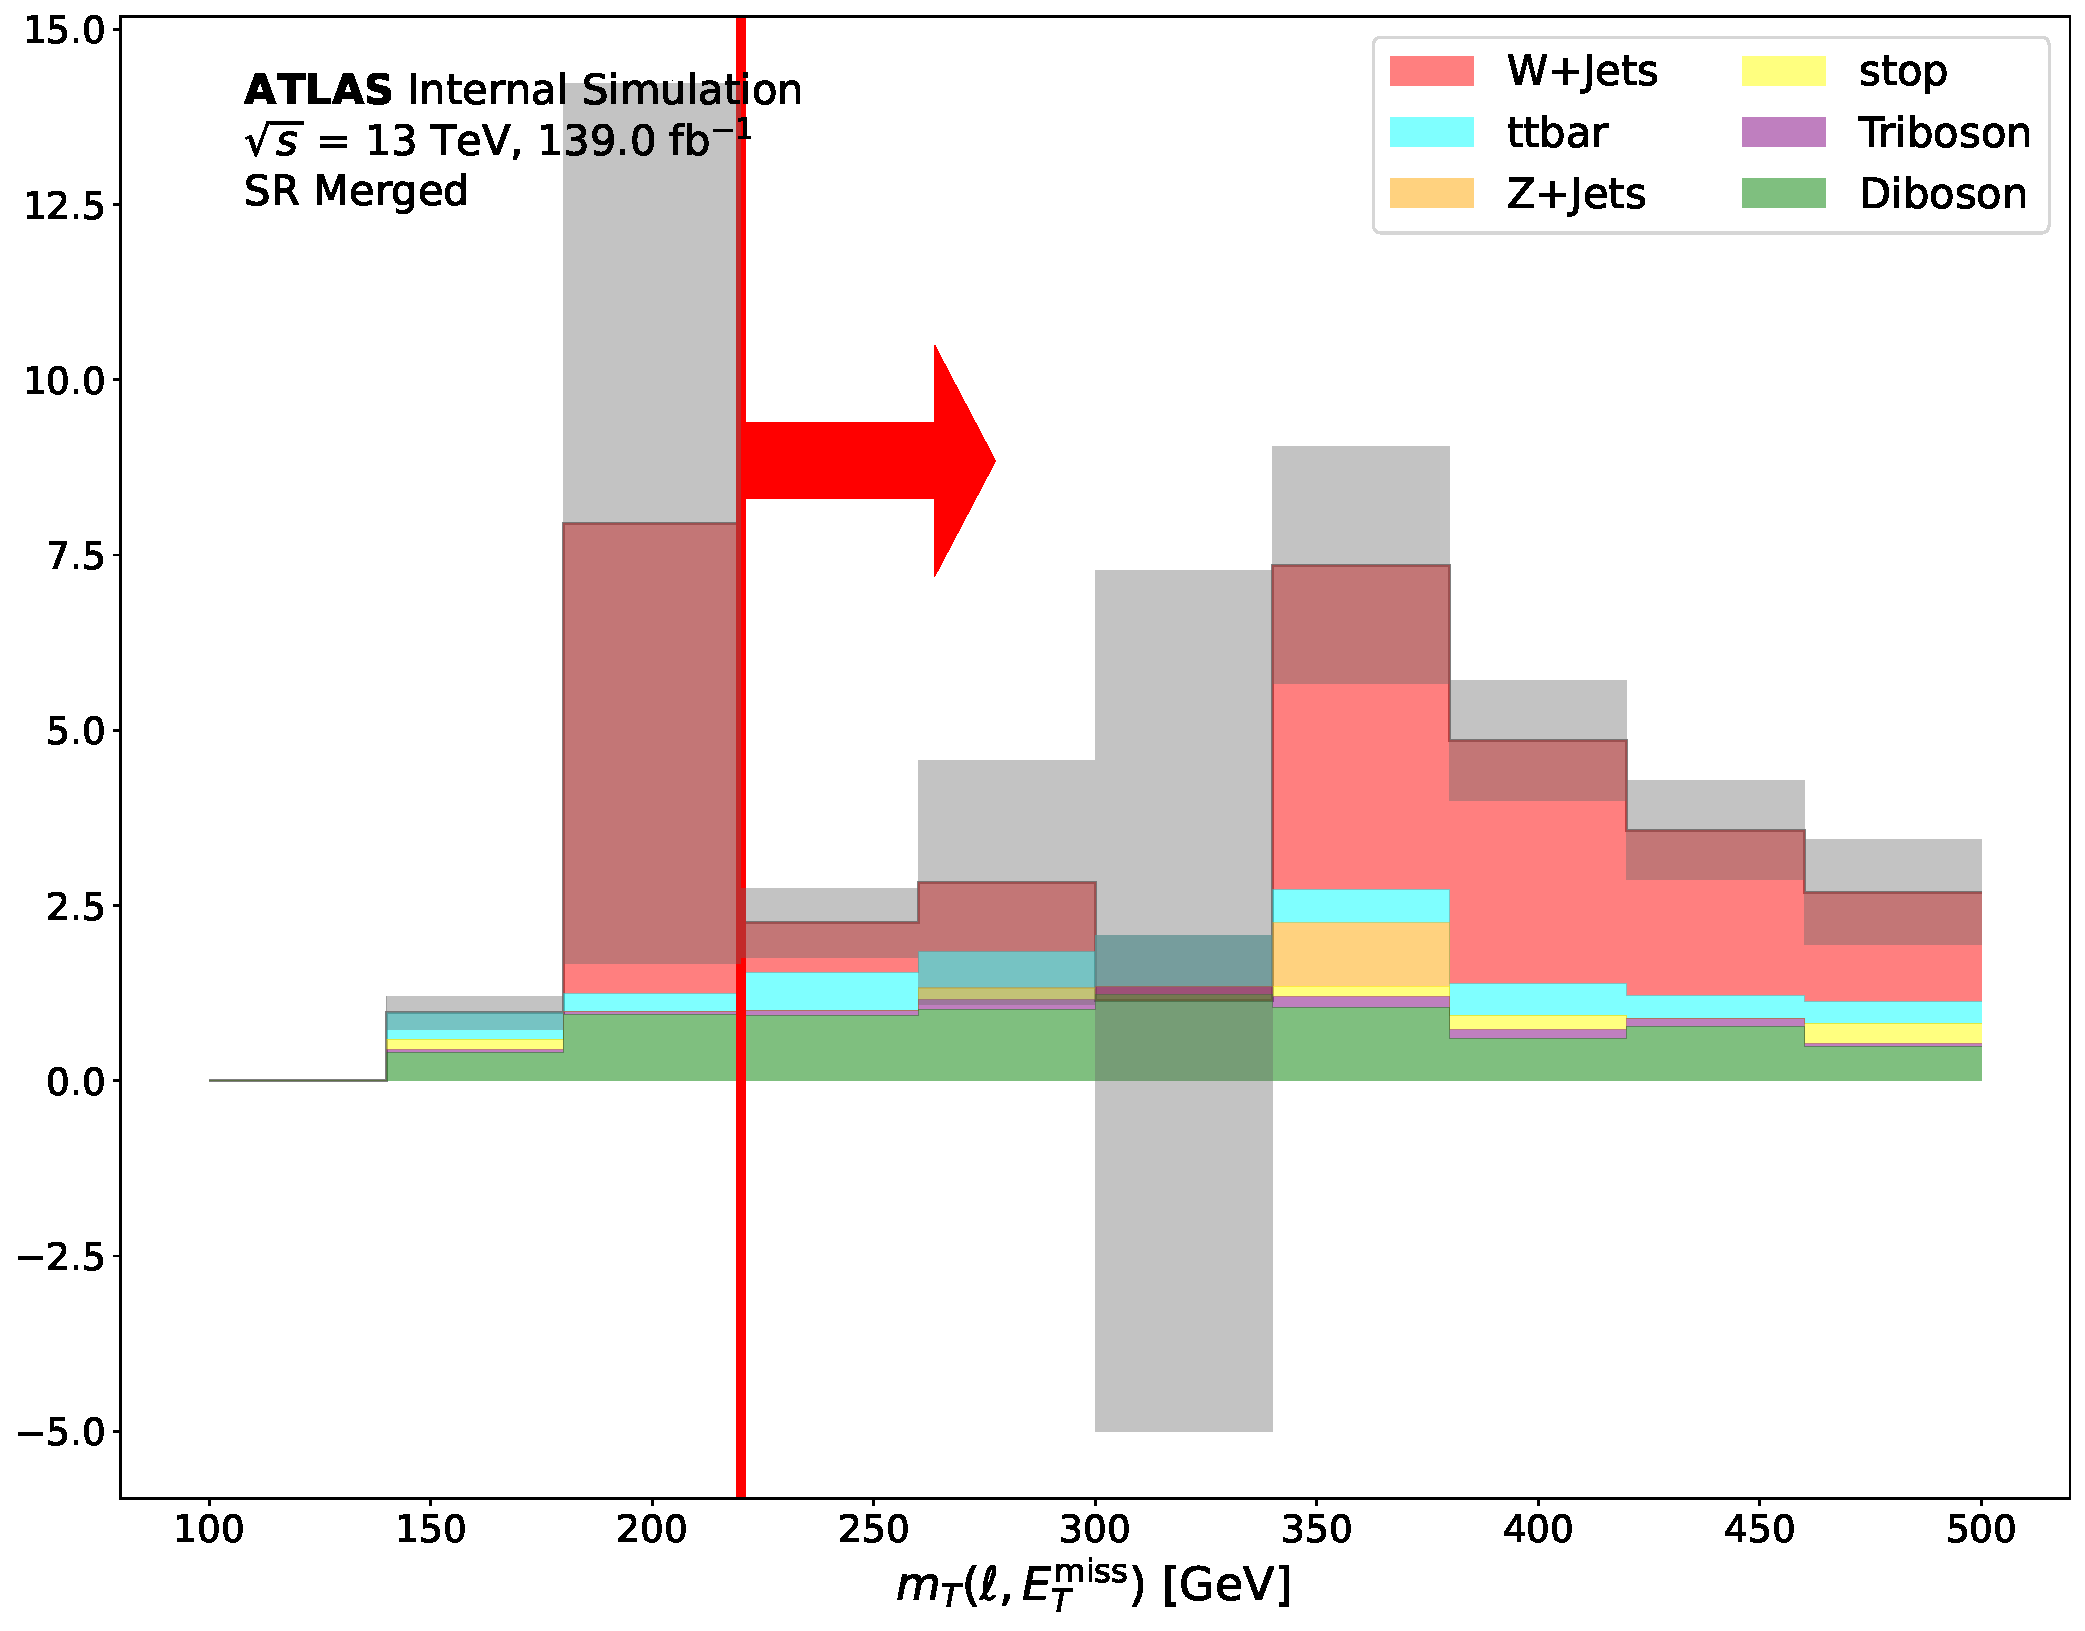
\includegraphics[width = 0.95\textwidth]{Figures/App_SR_CR_distributions/SR1L_Merged/mT_lep_met_N_1.pdf}
    \caption{\mtlepmet (merged SR)}
     \end{subfigure}
    \begin{subfigure}{0.45\textwidth}
     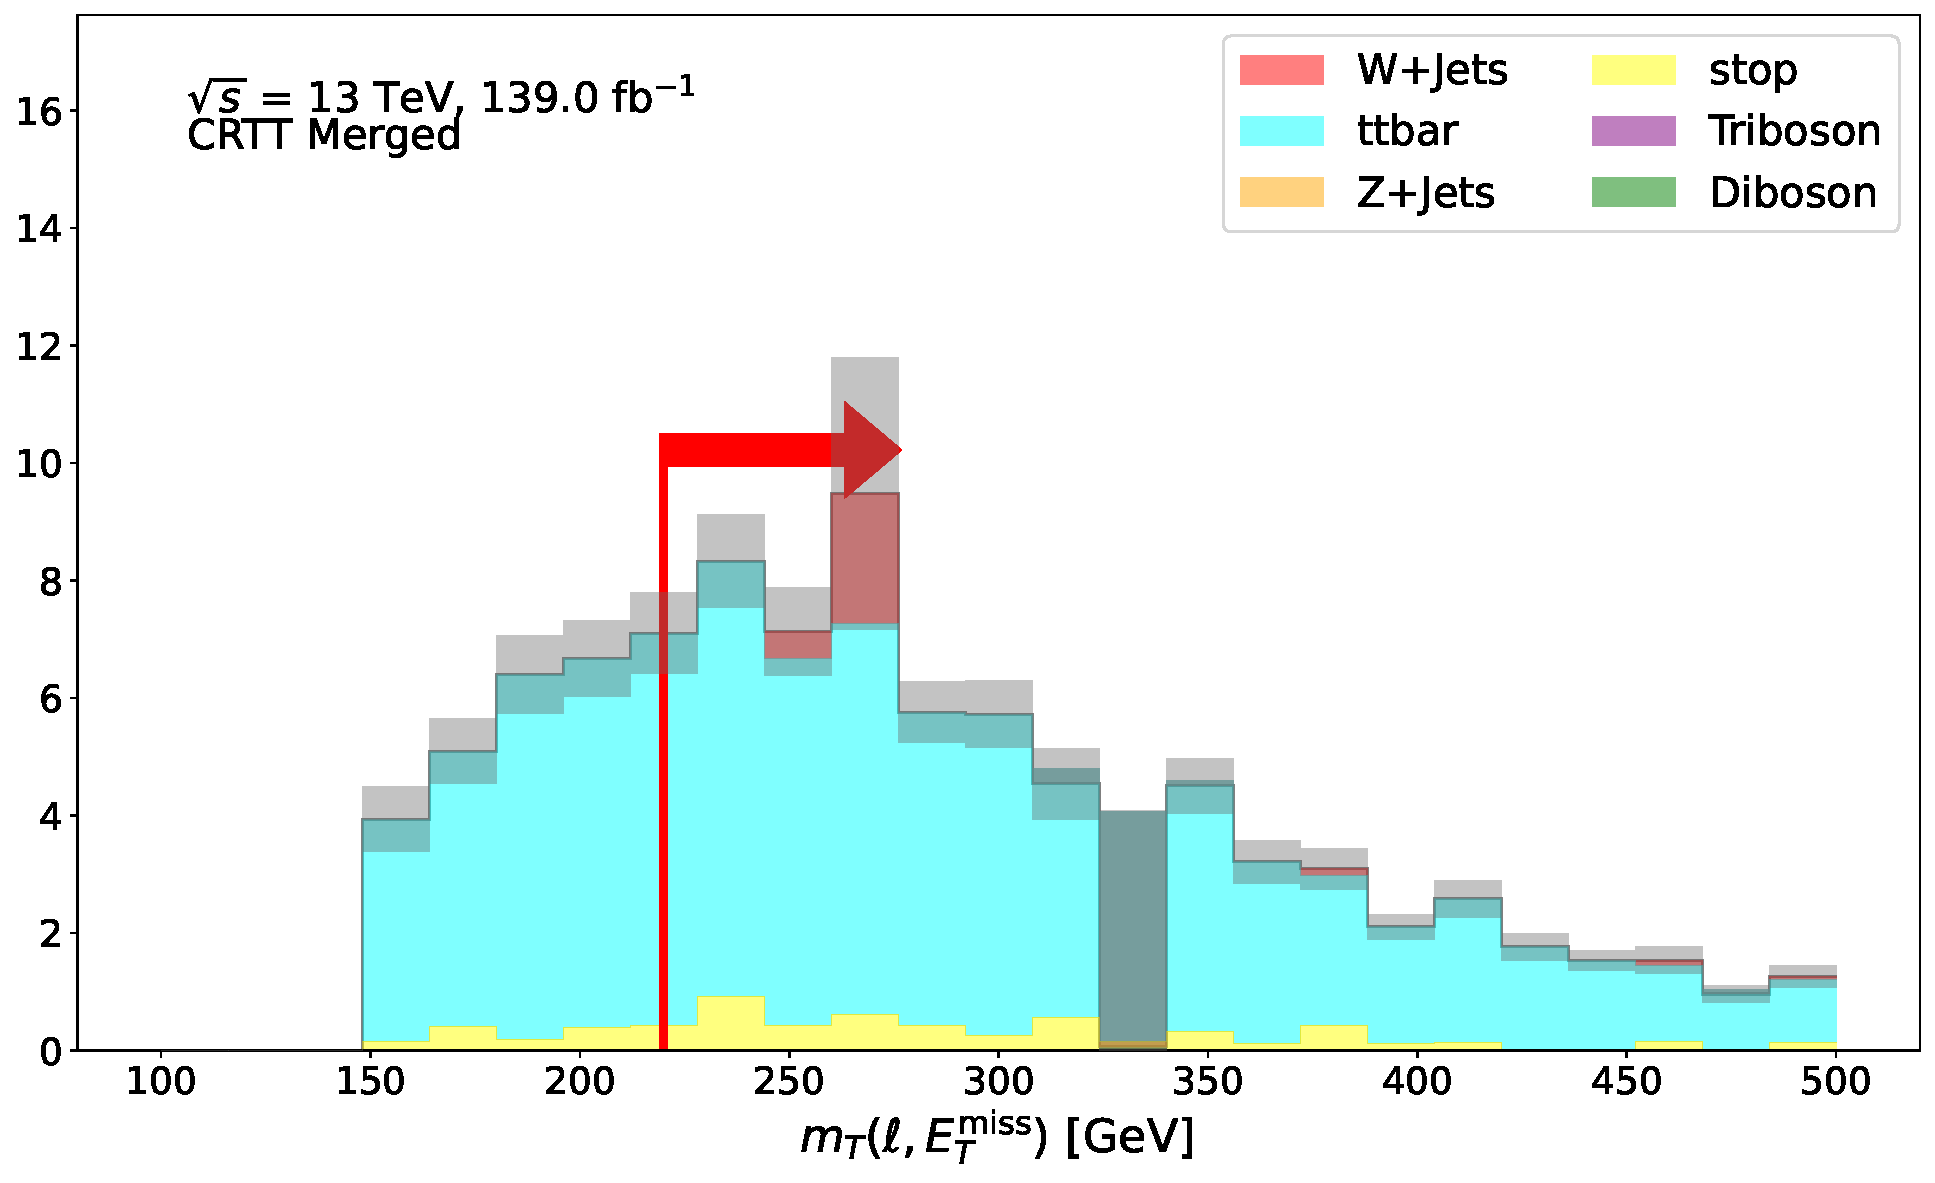
\includegraphics[width = 0.95\textwidth]{Figures/App_SR_CR_distributions/CRTT_Merged/mT_lep_met_N_1.pdf}
     \caption{\mtlepmet (merged \ttbar CR)}
     \end{subfigure}

      \begin{subfigure}{0.45\textwidth}
     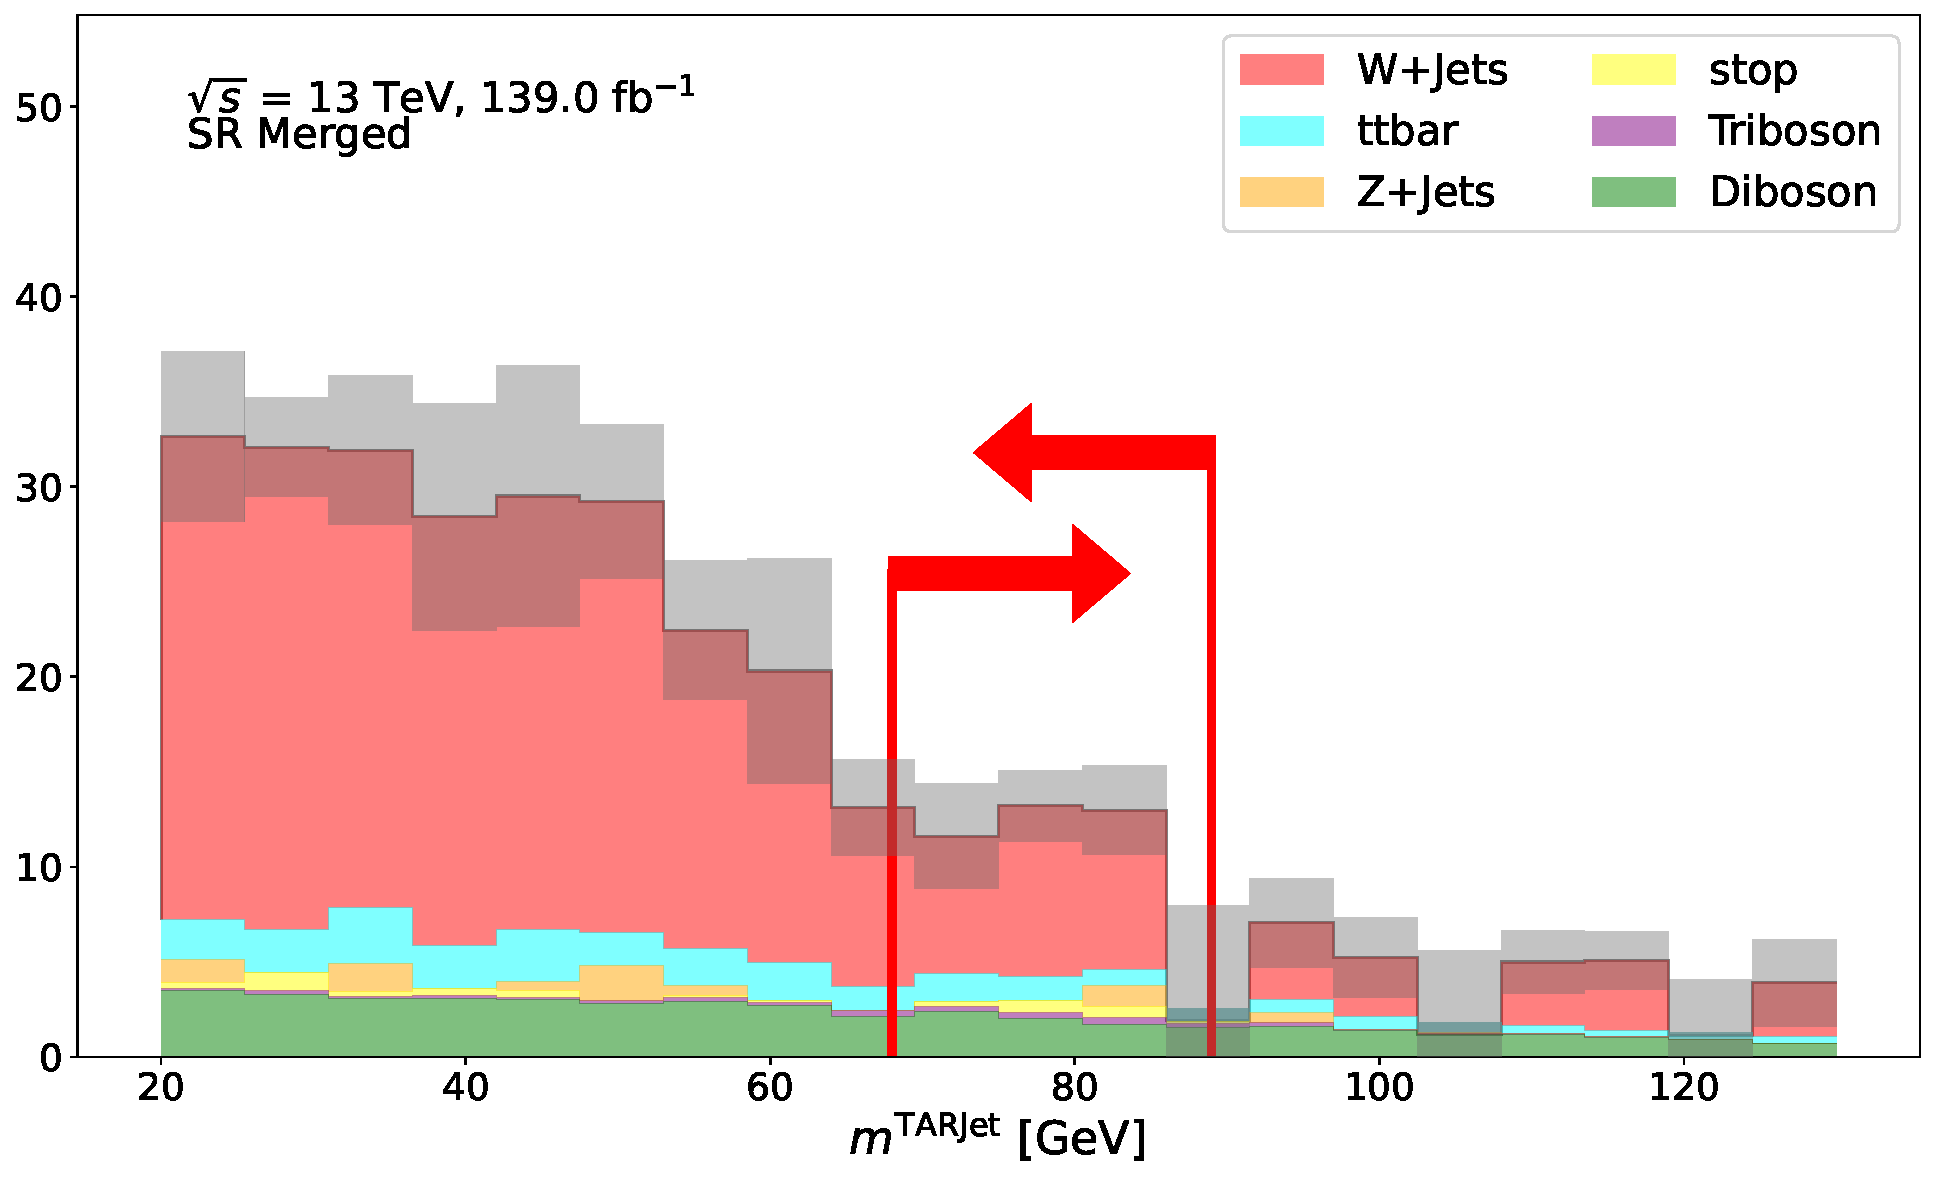
\includegraphics[width = 0.95\textwidth]{Figures/App_SR_CR_distributions/SR1L_Merged/TARJets10_mTAR0_N_1.pdf}
    \caption{\mTAR (merged SR)}
     \end{subfigure}
    \begin{subfigure}{0.45\textwidth}
     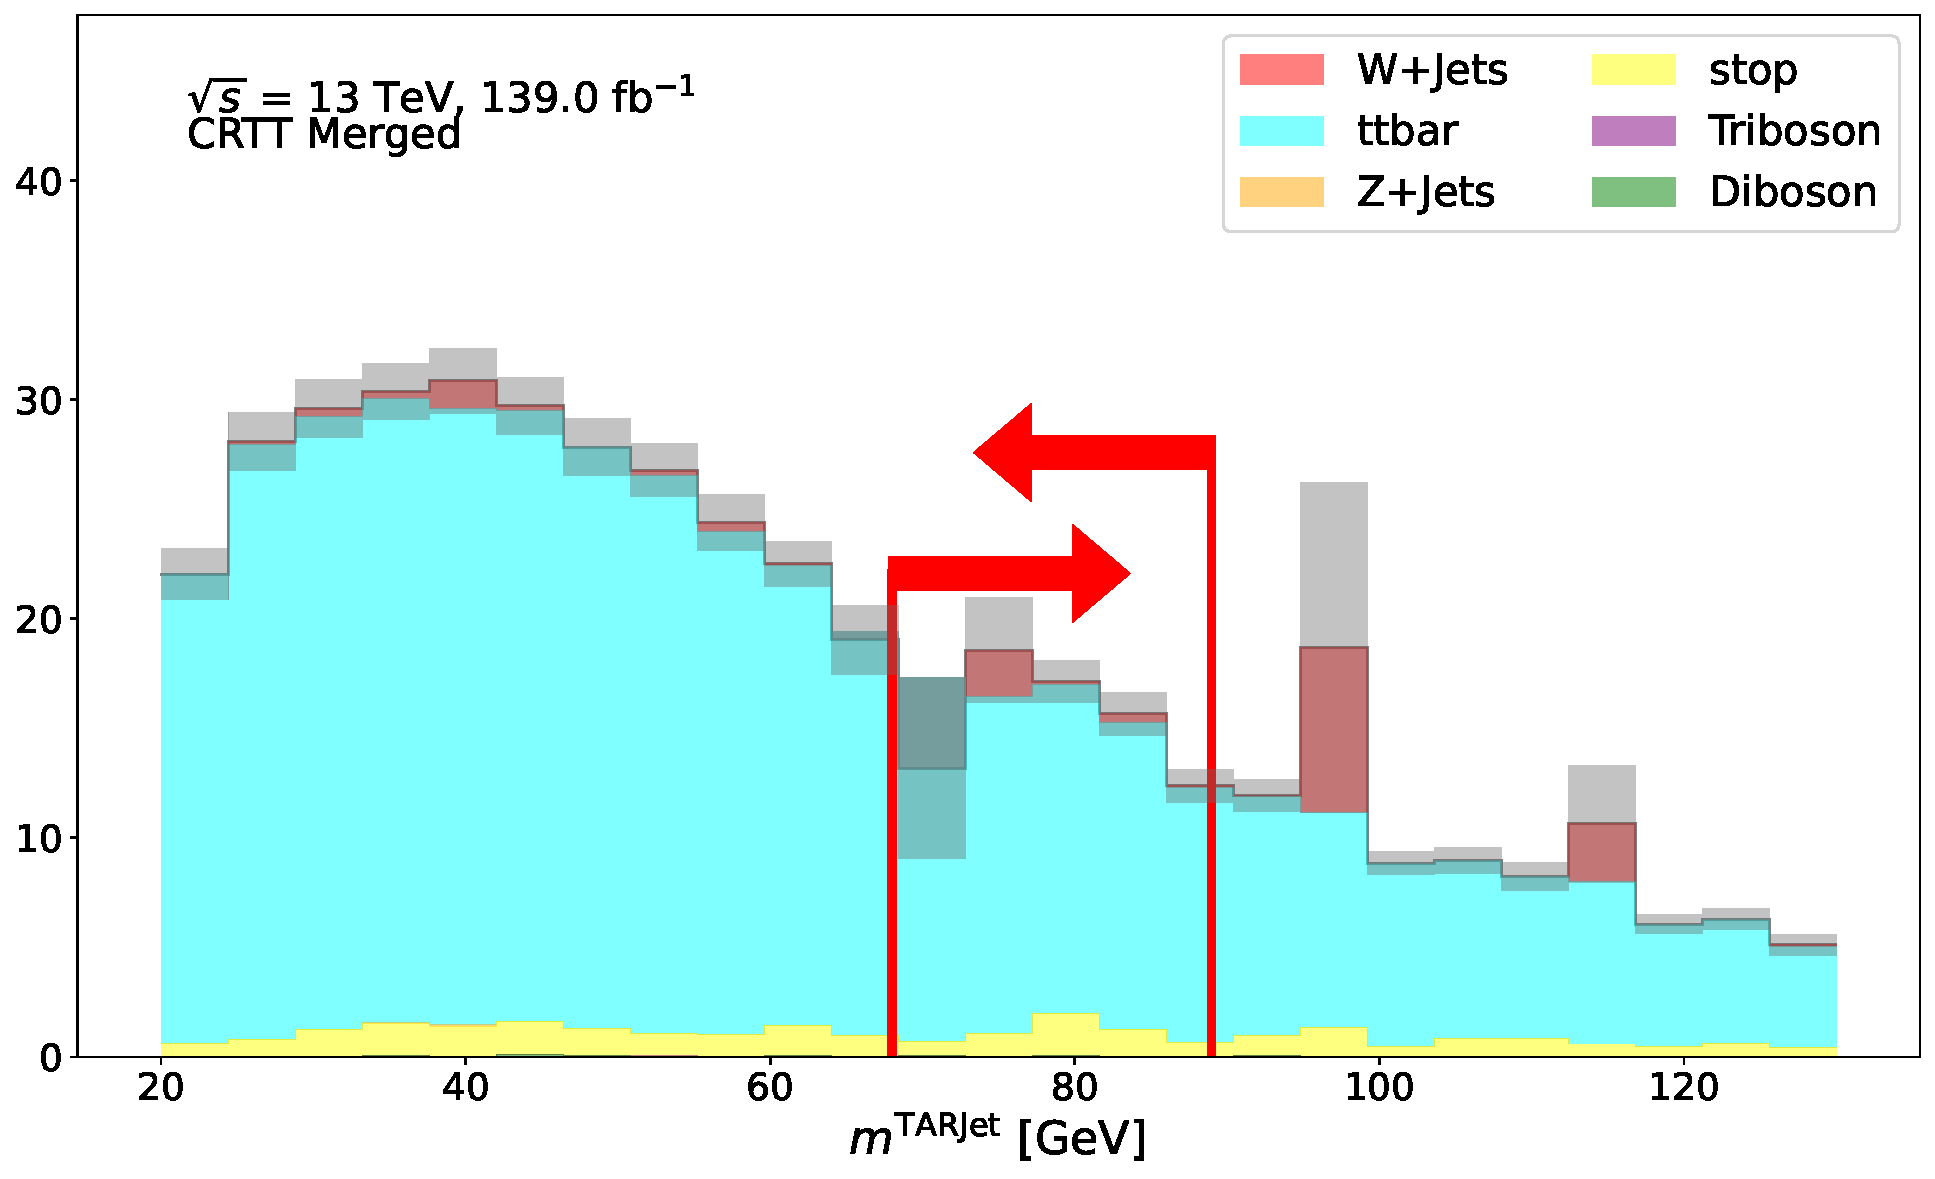
\includegraphics[width = 0.95\textwidth]{Figures/App_SR_CR_distributions/CRTT_Merged/TARJets10_mTAR0_N_1.pdf}
     \caption{\mTAR (merged \ttbar CR)}
     \end{subfigure}

 \begin{subfigure}{0.45\textwidth}
     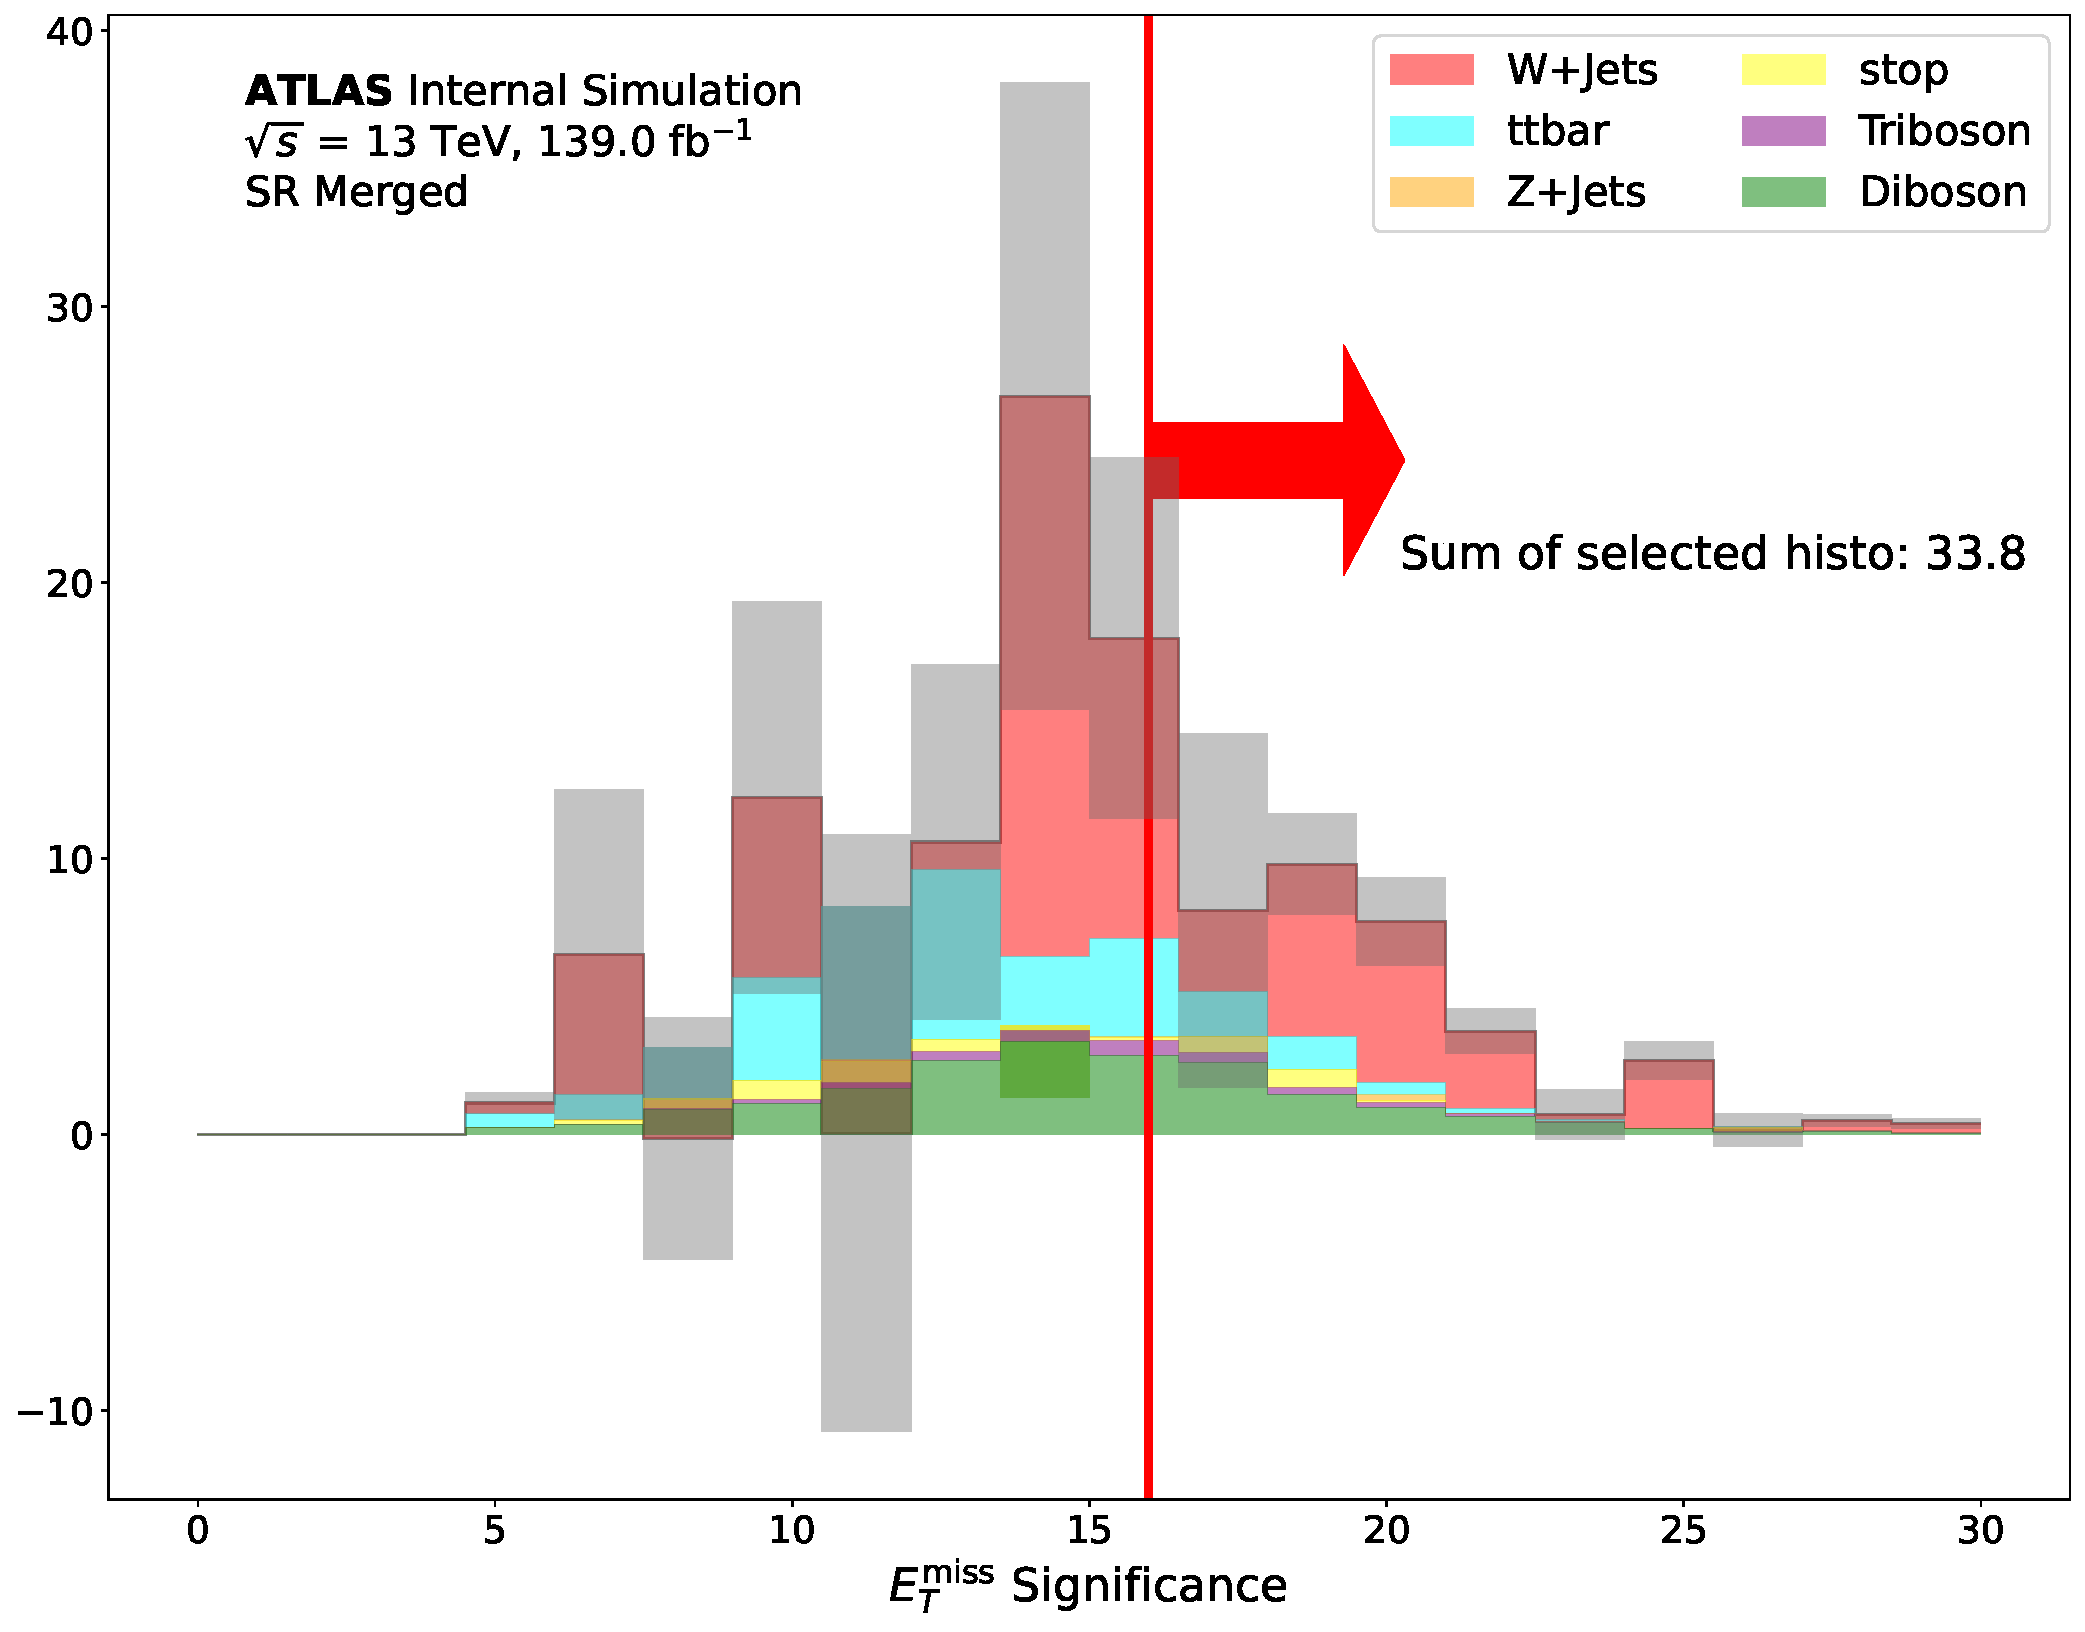
\includegraphics[width = 0.95\textwidth]{Figures/App_SR_CR_distributions/SR1L_Merged/MetTST_Significance_N_1.pdf}
    \caption{\metsig (merged SR)}
     \end{subfigure}
    \begin{subfigure}{0.45\textwidth}
     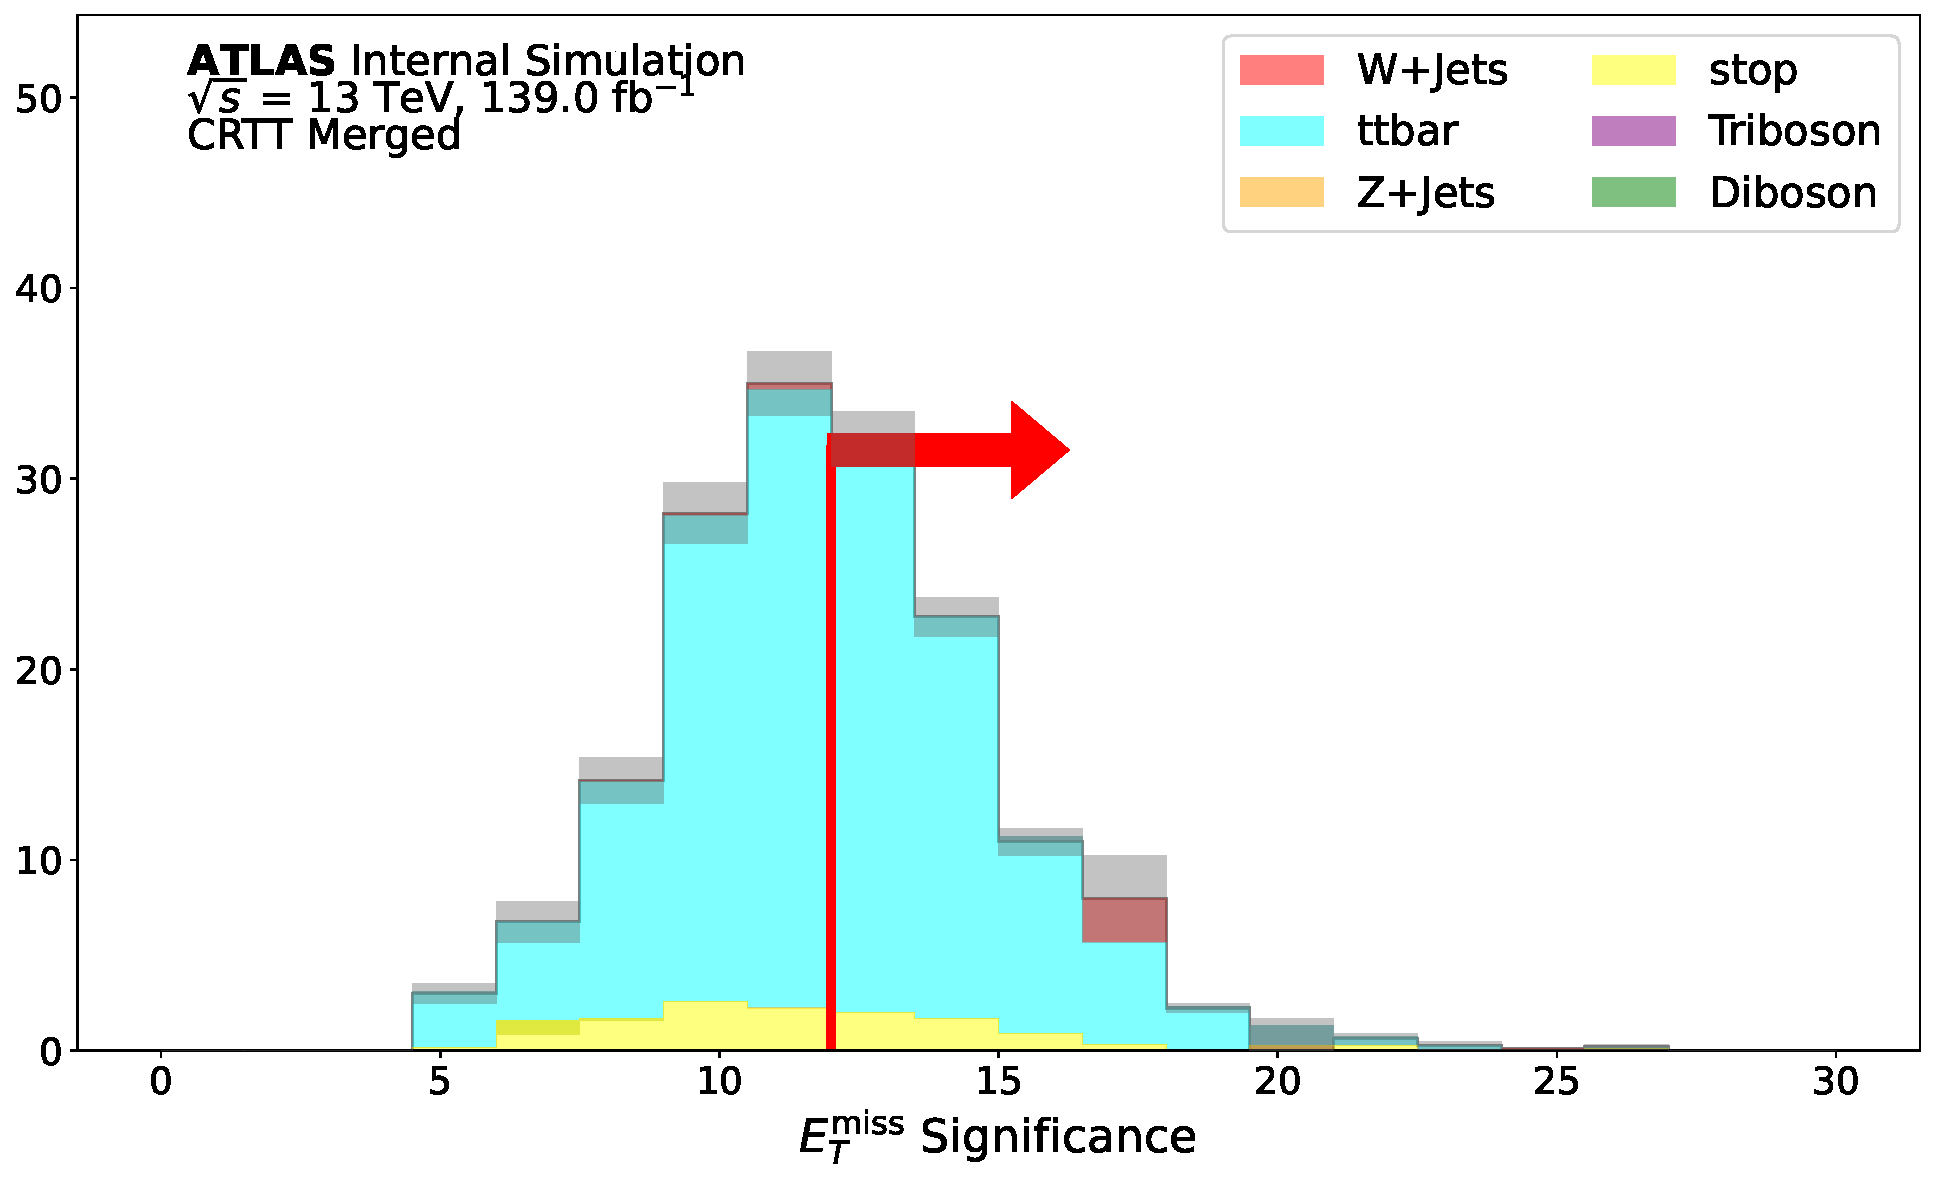
\includegraphics[width = 0.95\textwidth]{Figures/App_SR_CR_distributions/CRTT_Merged/MetTST_Significance_N_1.pdf}
     \caption{\metsig (merged \ttbar CR)}
     \end{subfigure}
      \caption{Comparison of N-1 distributions for kinematic variables of interest between the SR and the \ttbar CR in the merged category. Grey bands show statistical uncertainty on the background estimate.}
       \end{figure}
    \begin{figure}[htbp]\ContinuedFloat
  \begin{subfigure}{0.45\textwidth}
     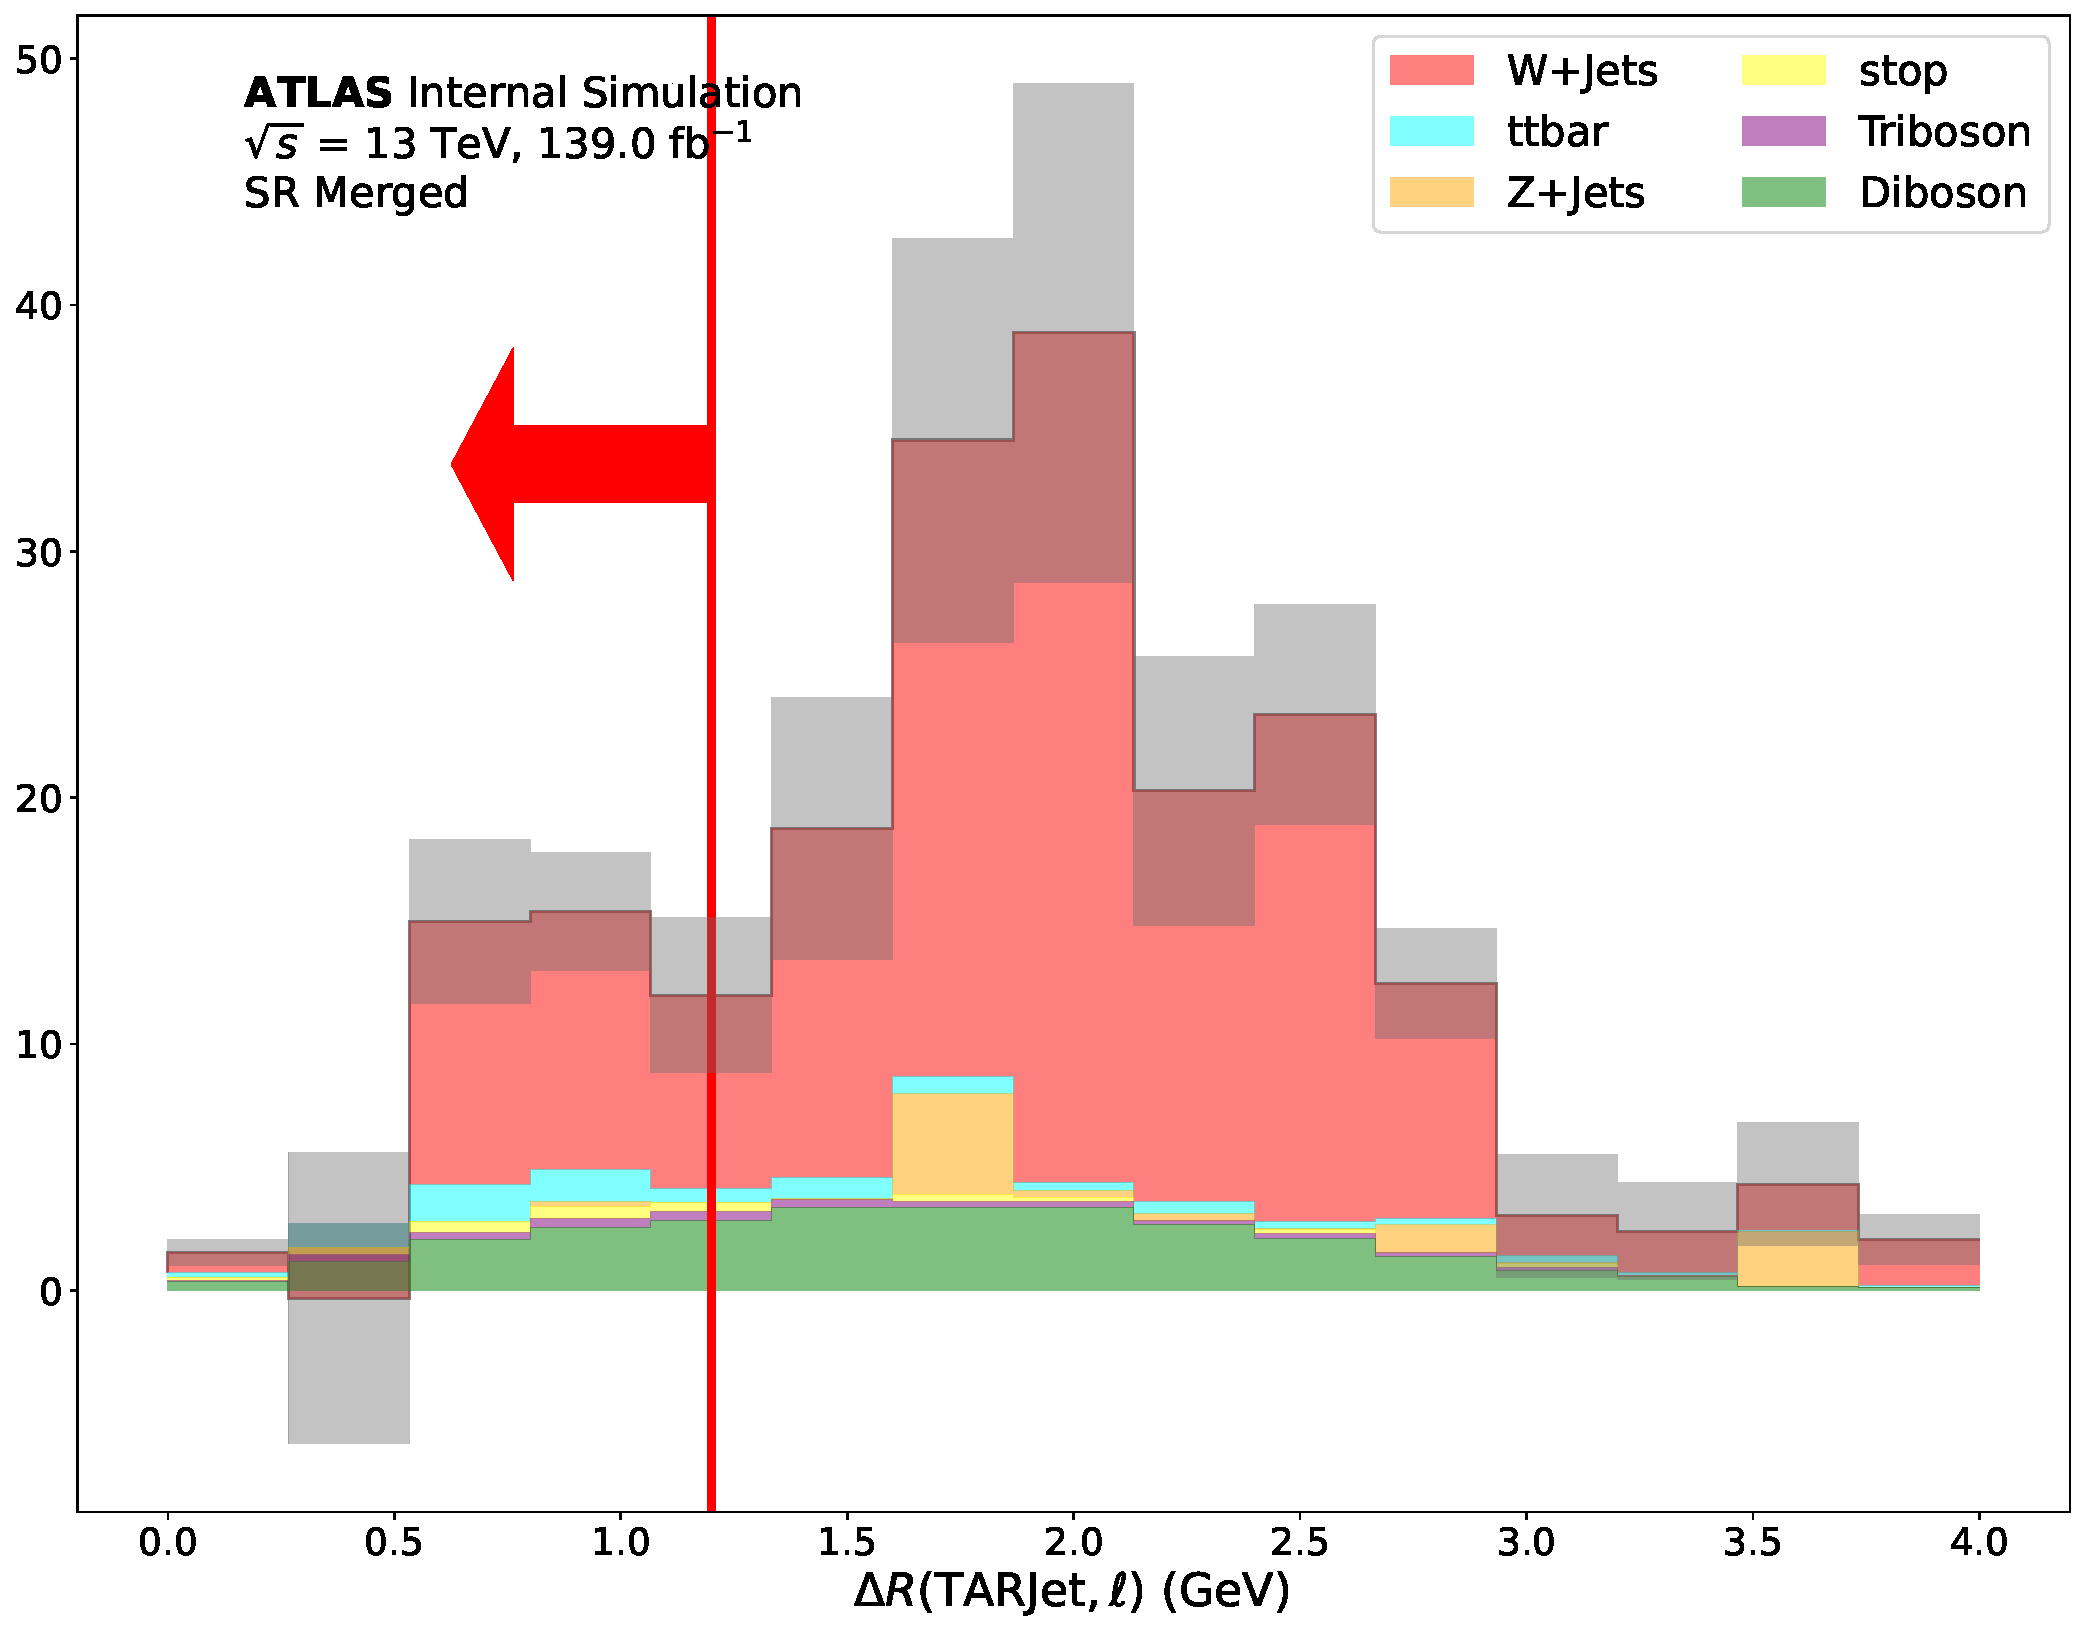
\includegraphics[width = 0.95\textwidth]{Figures/App_SR_CR_distributions/SR1L_Merged/dR_lep_TARJets10_N_1.pdf}
    \caption{\drTARl (merged SR)}
     \end{subfigure}
    \begin{subfigure}{0.45\textwidth}
     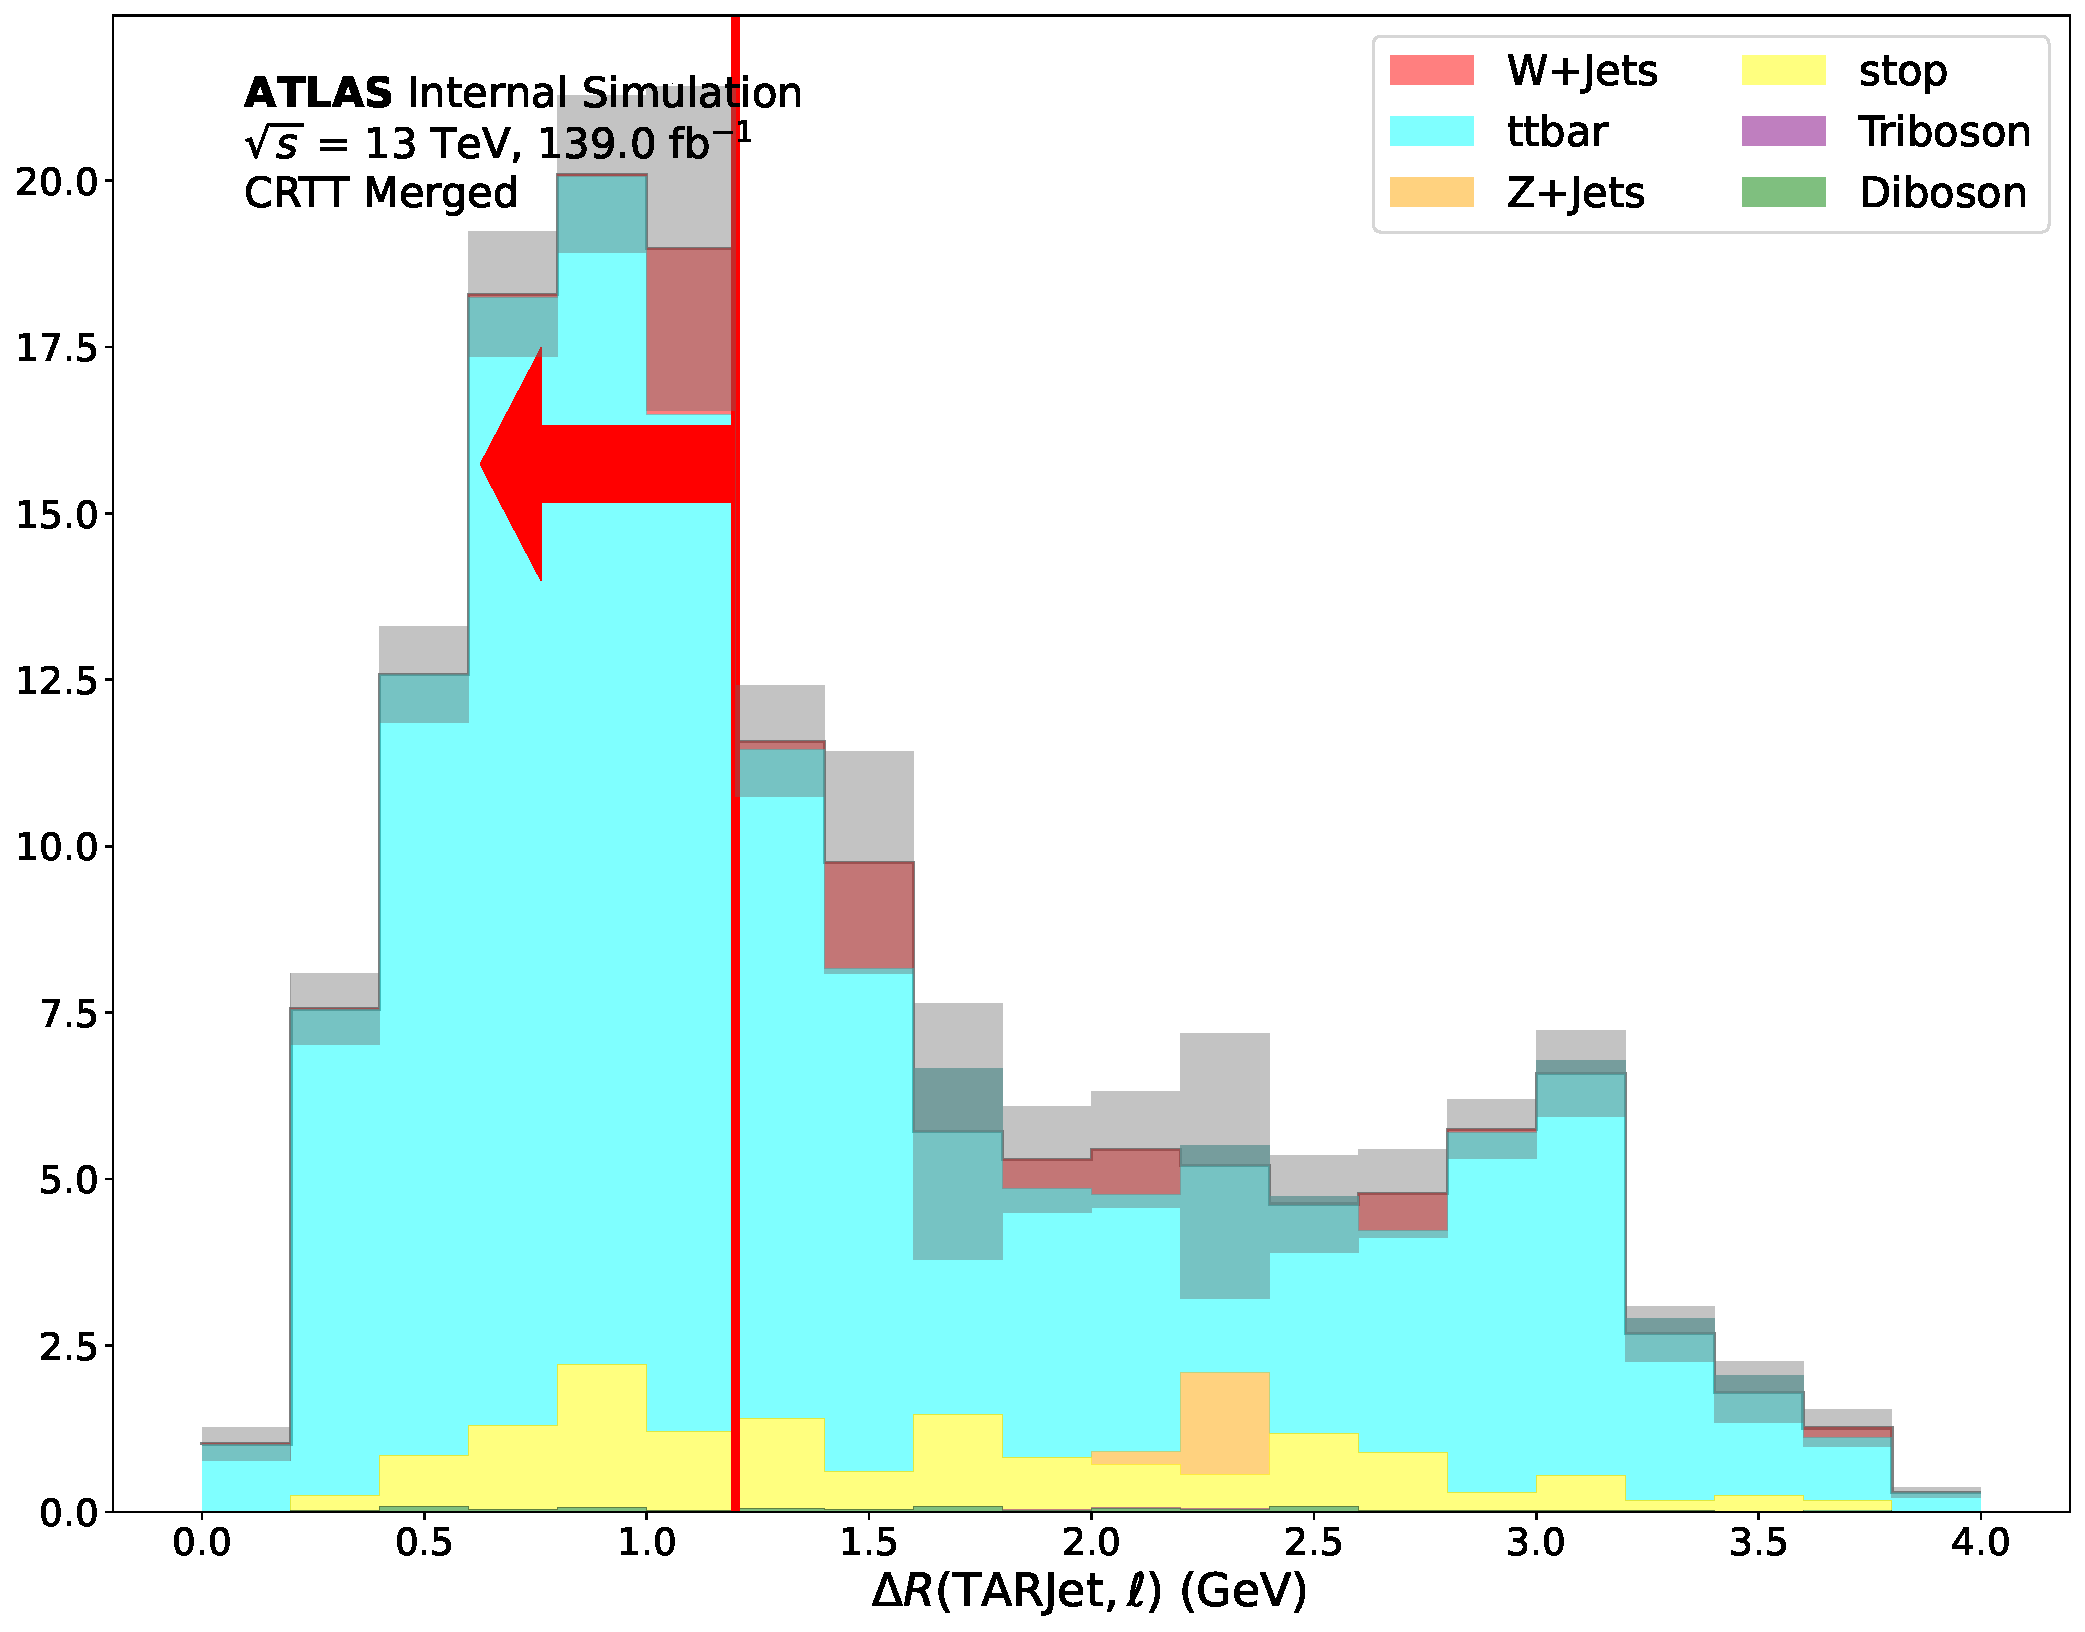
\includegraphics[width = 0.95\textwidth]{Figures/App_SR_CR_distributions/CRTT_Merged/dR_lep_TARJets10_N_1.pdf}
     \caption{\drTARl (merged \ttbar CR)}
     \end{subfigure}

   \begin{subfigure}{0.45\textwidth}
     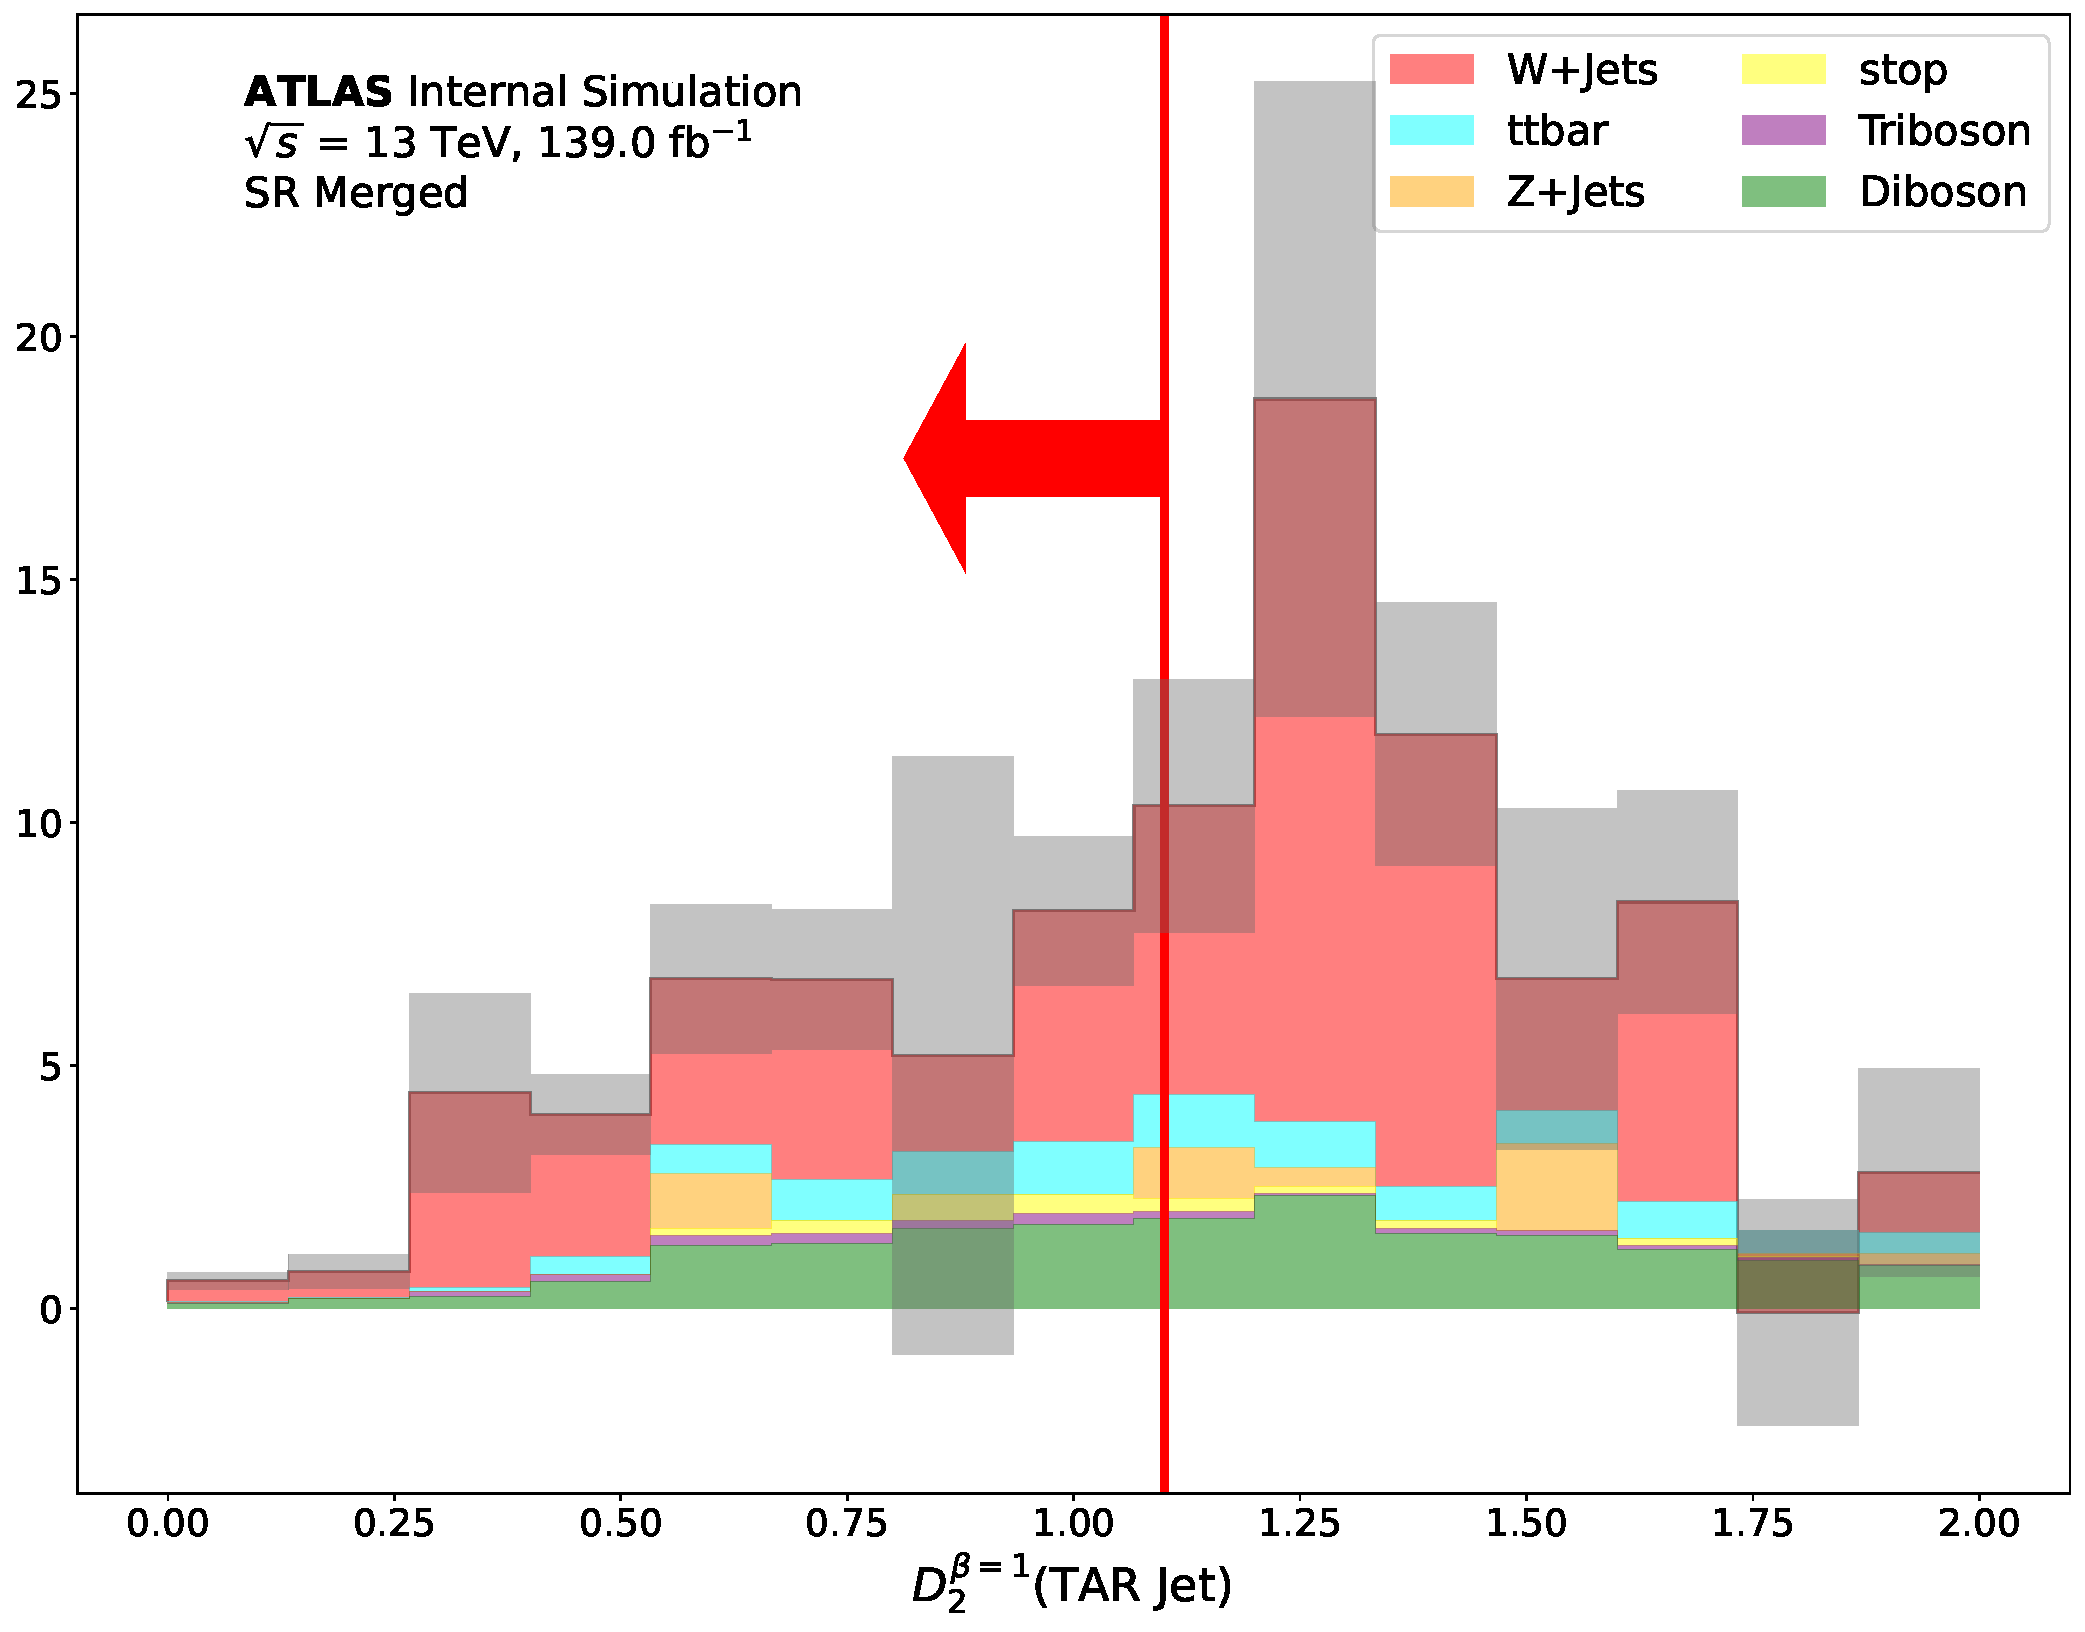
\includegraphics[width = 0.95\textwidth]{Figures/App_SR_CR_distributions/SR1L_Merged/TARJets10_TAR_D20_N_1.pdf}
    \caption{\DtwoTAR (merged SR)}
     \end{subfigure}
    \begin{subfigure}{0.45\textwidth}
     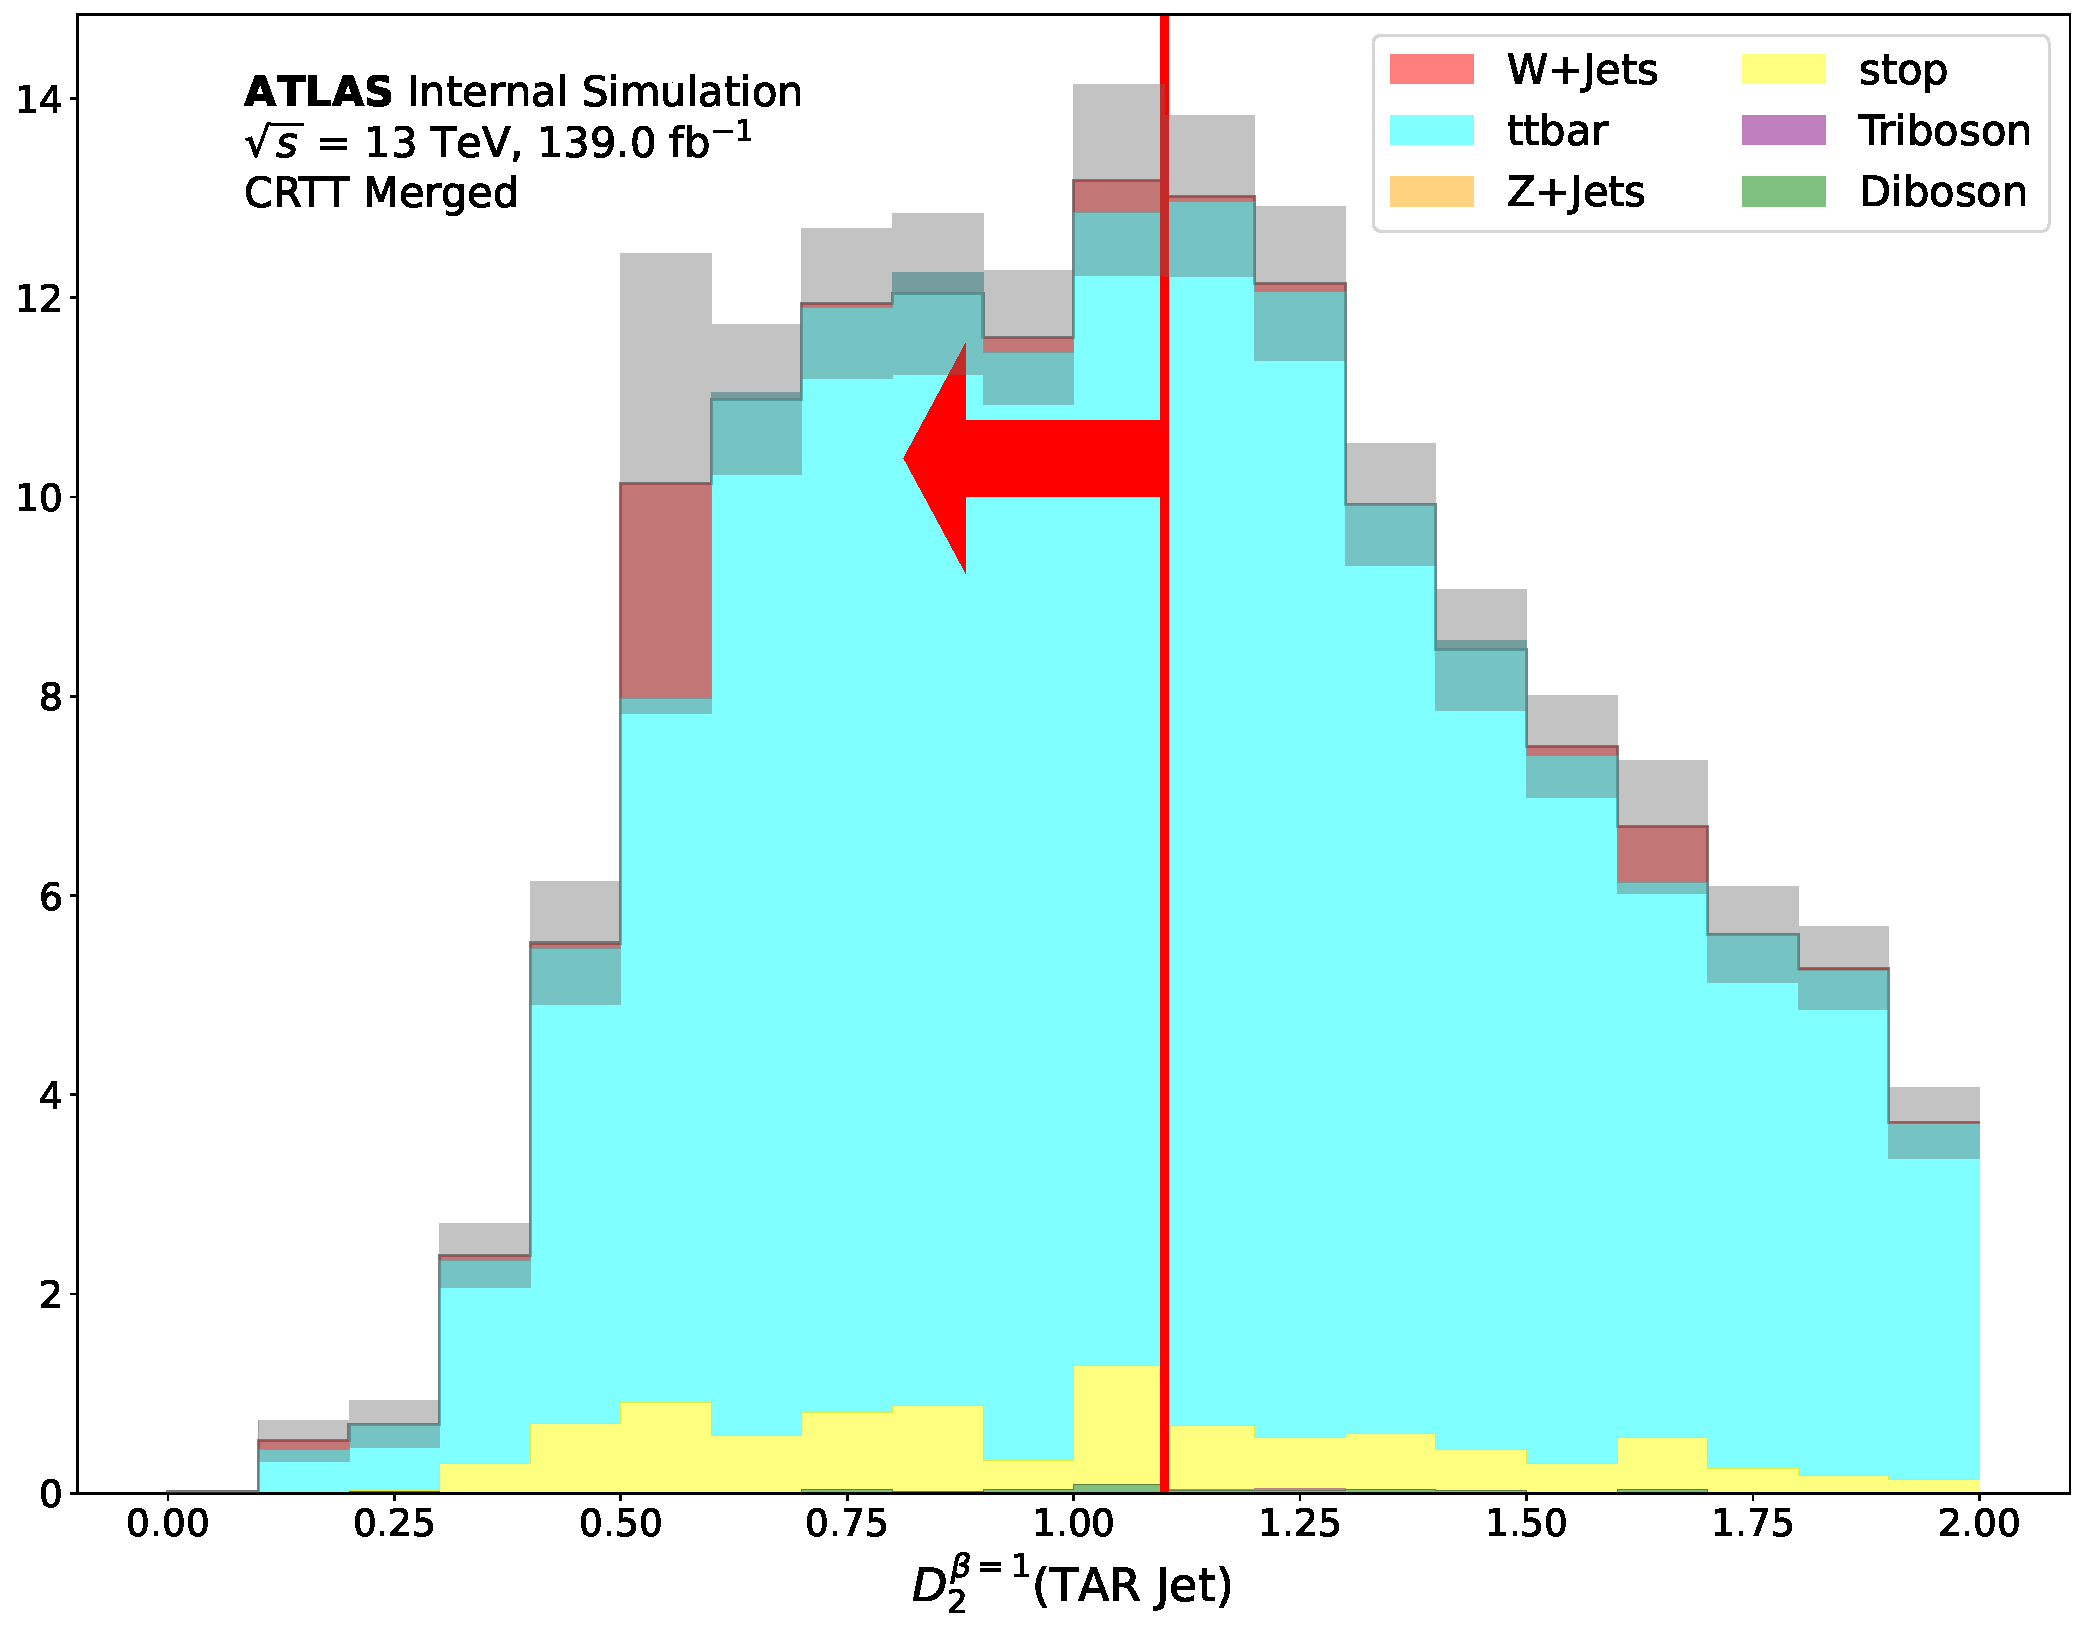
\includegraphics[width = 0.95\textwidth]{Figures/App_SR_CR_distributions/CRTT_Merged/TARJets10_TAR_D20_N_1.pdf}
     \caption{\DtwoTAR (merged \ttbar CR)}
     \end{subfigure}

   \begin{subfigure}{0.45\textwidth}
     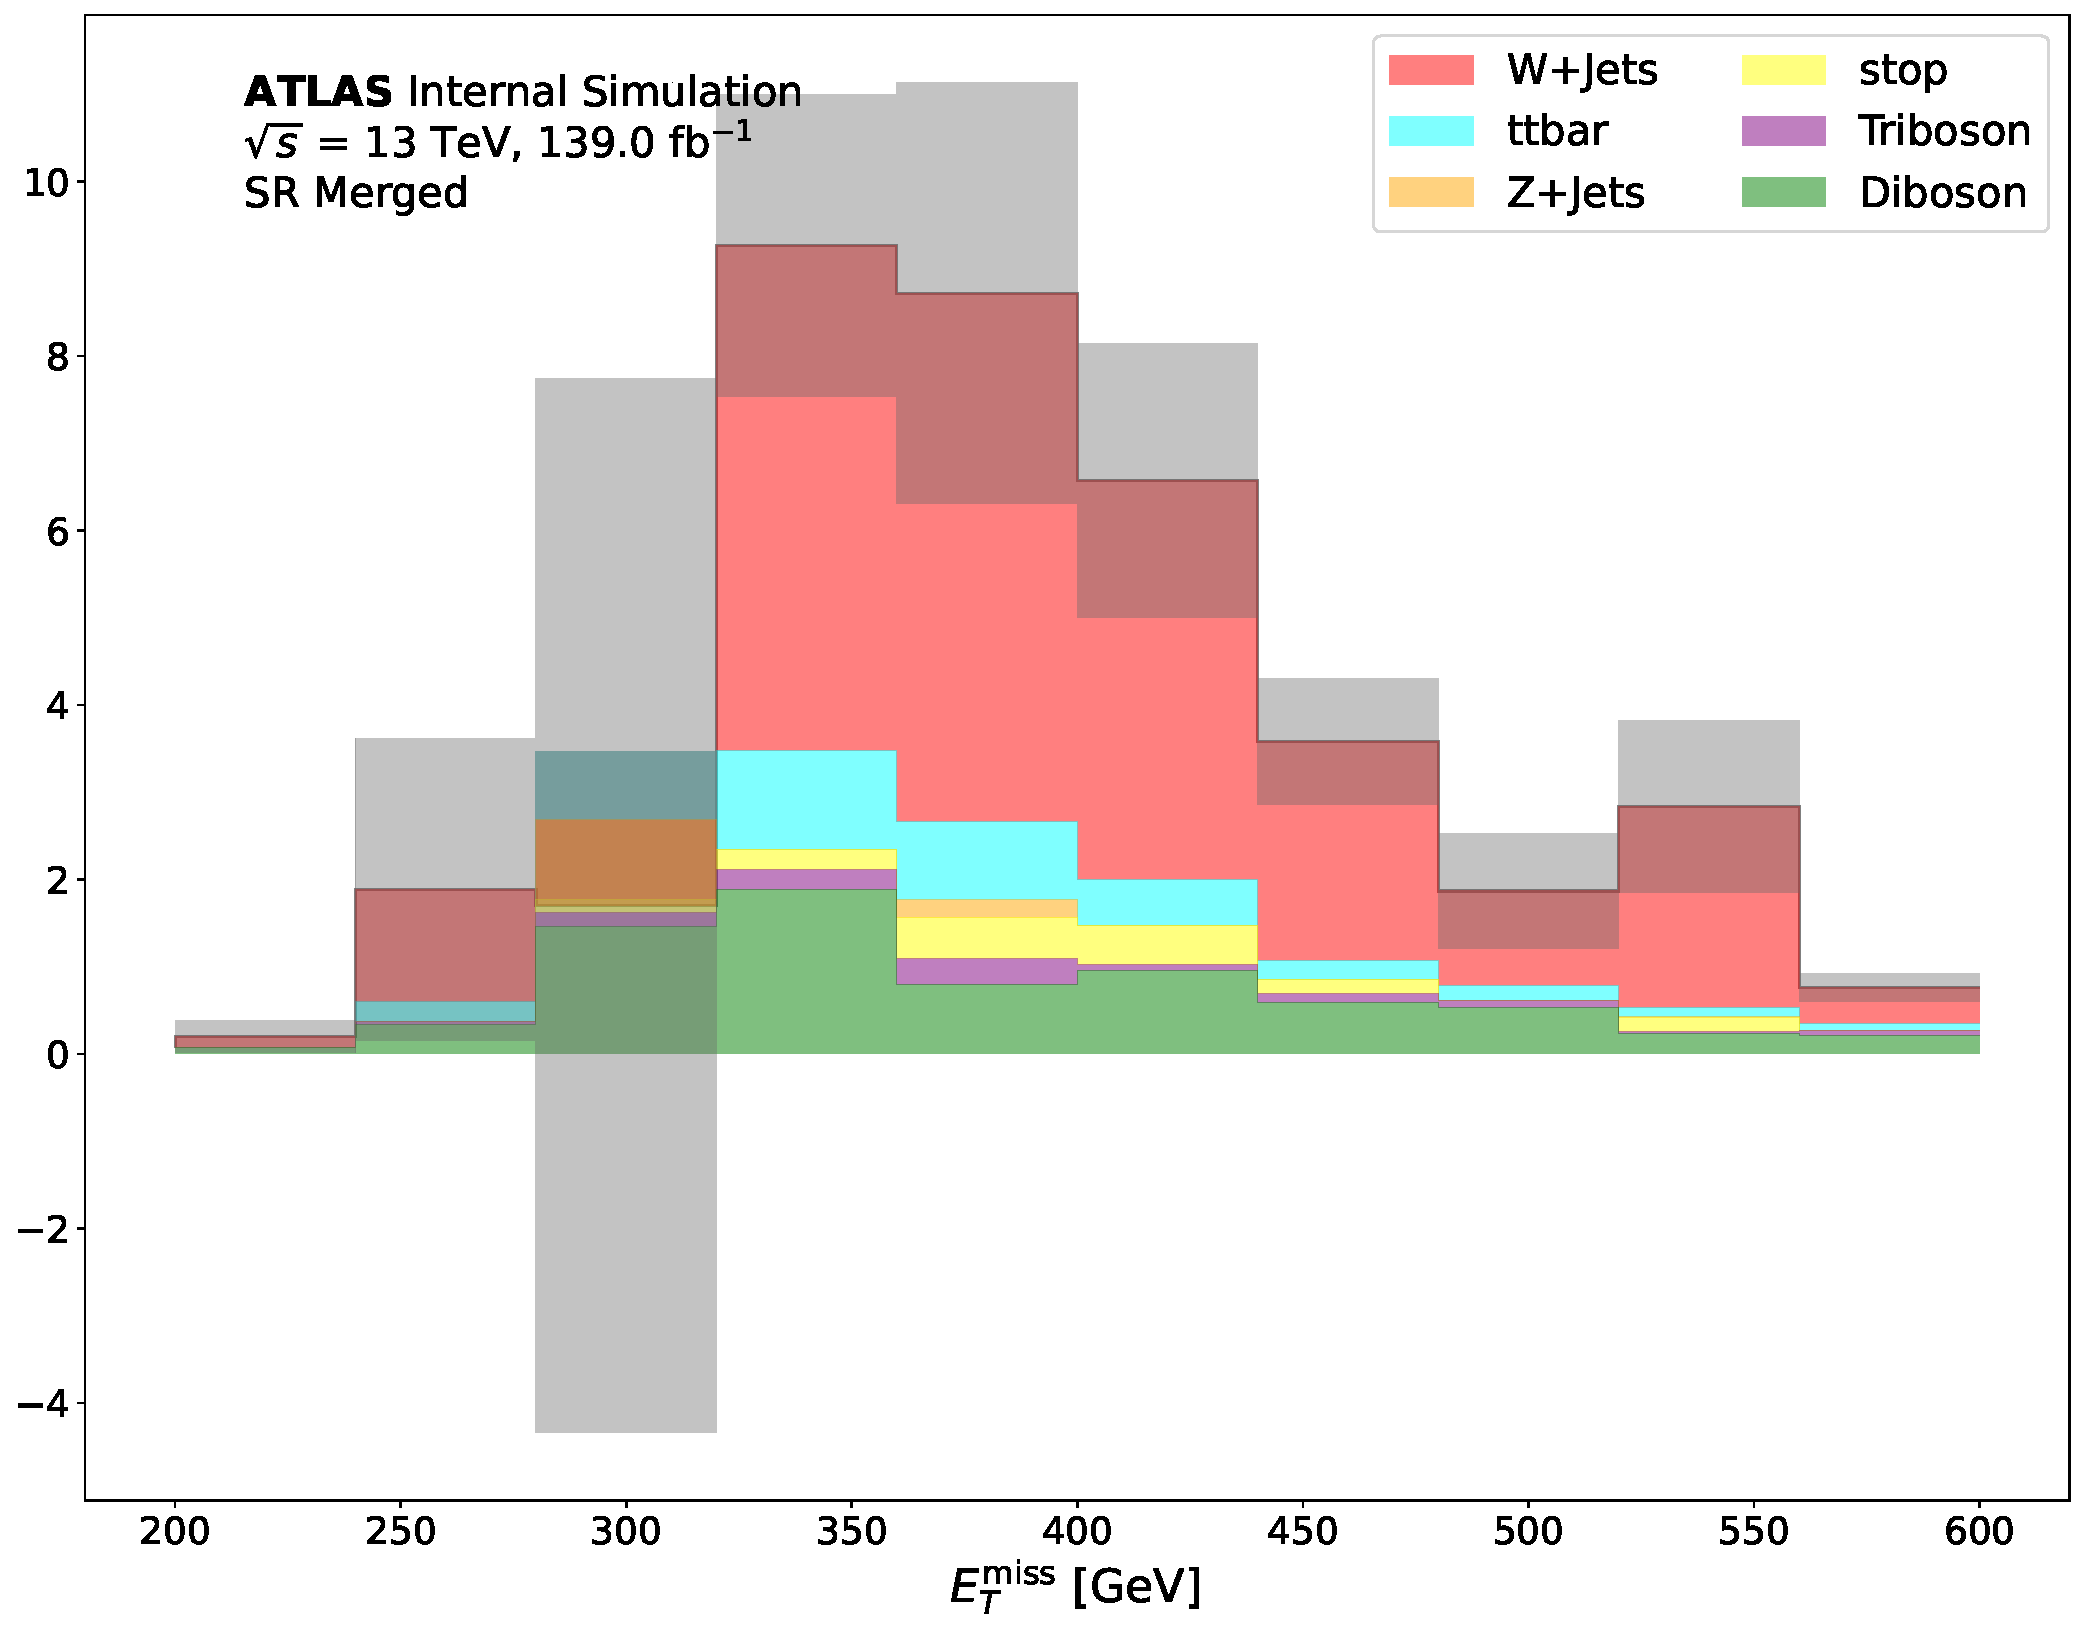
\includegraphics[width = 0.95\textwidth]{Figures/App_SR_CR_distributions/SR1L_Merged/MetTST_met_N_1.pdf}
    \caption{\met (merged SR)}
     \end{subfigure}
    \begin{subfigure}{0.45\textwidth}
     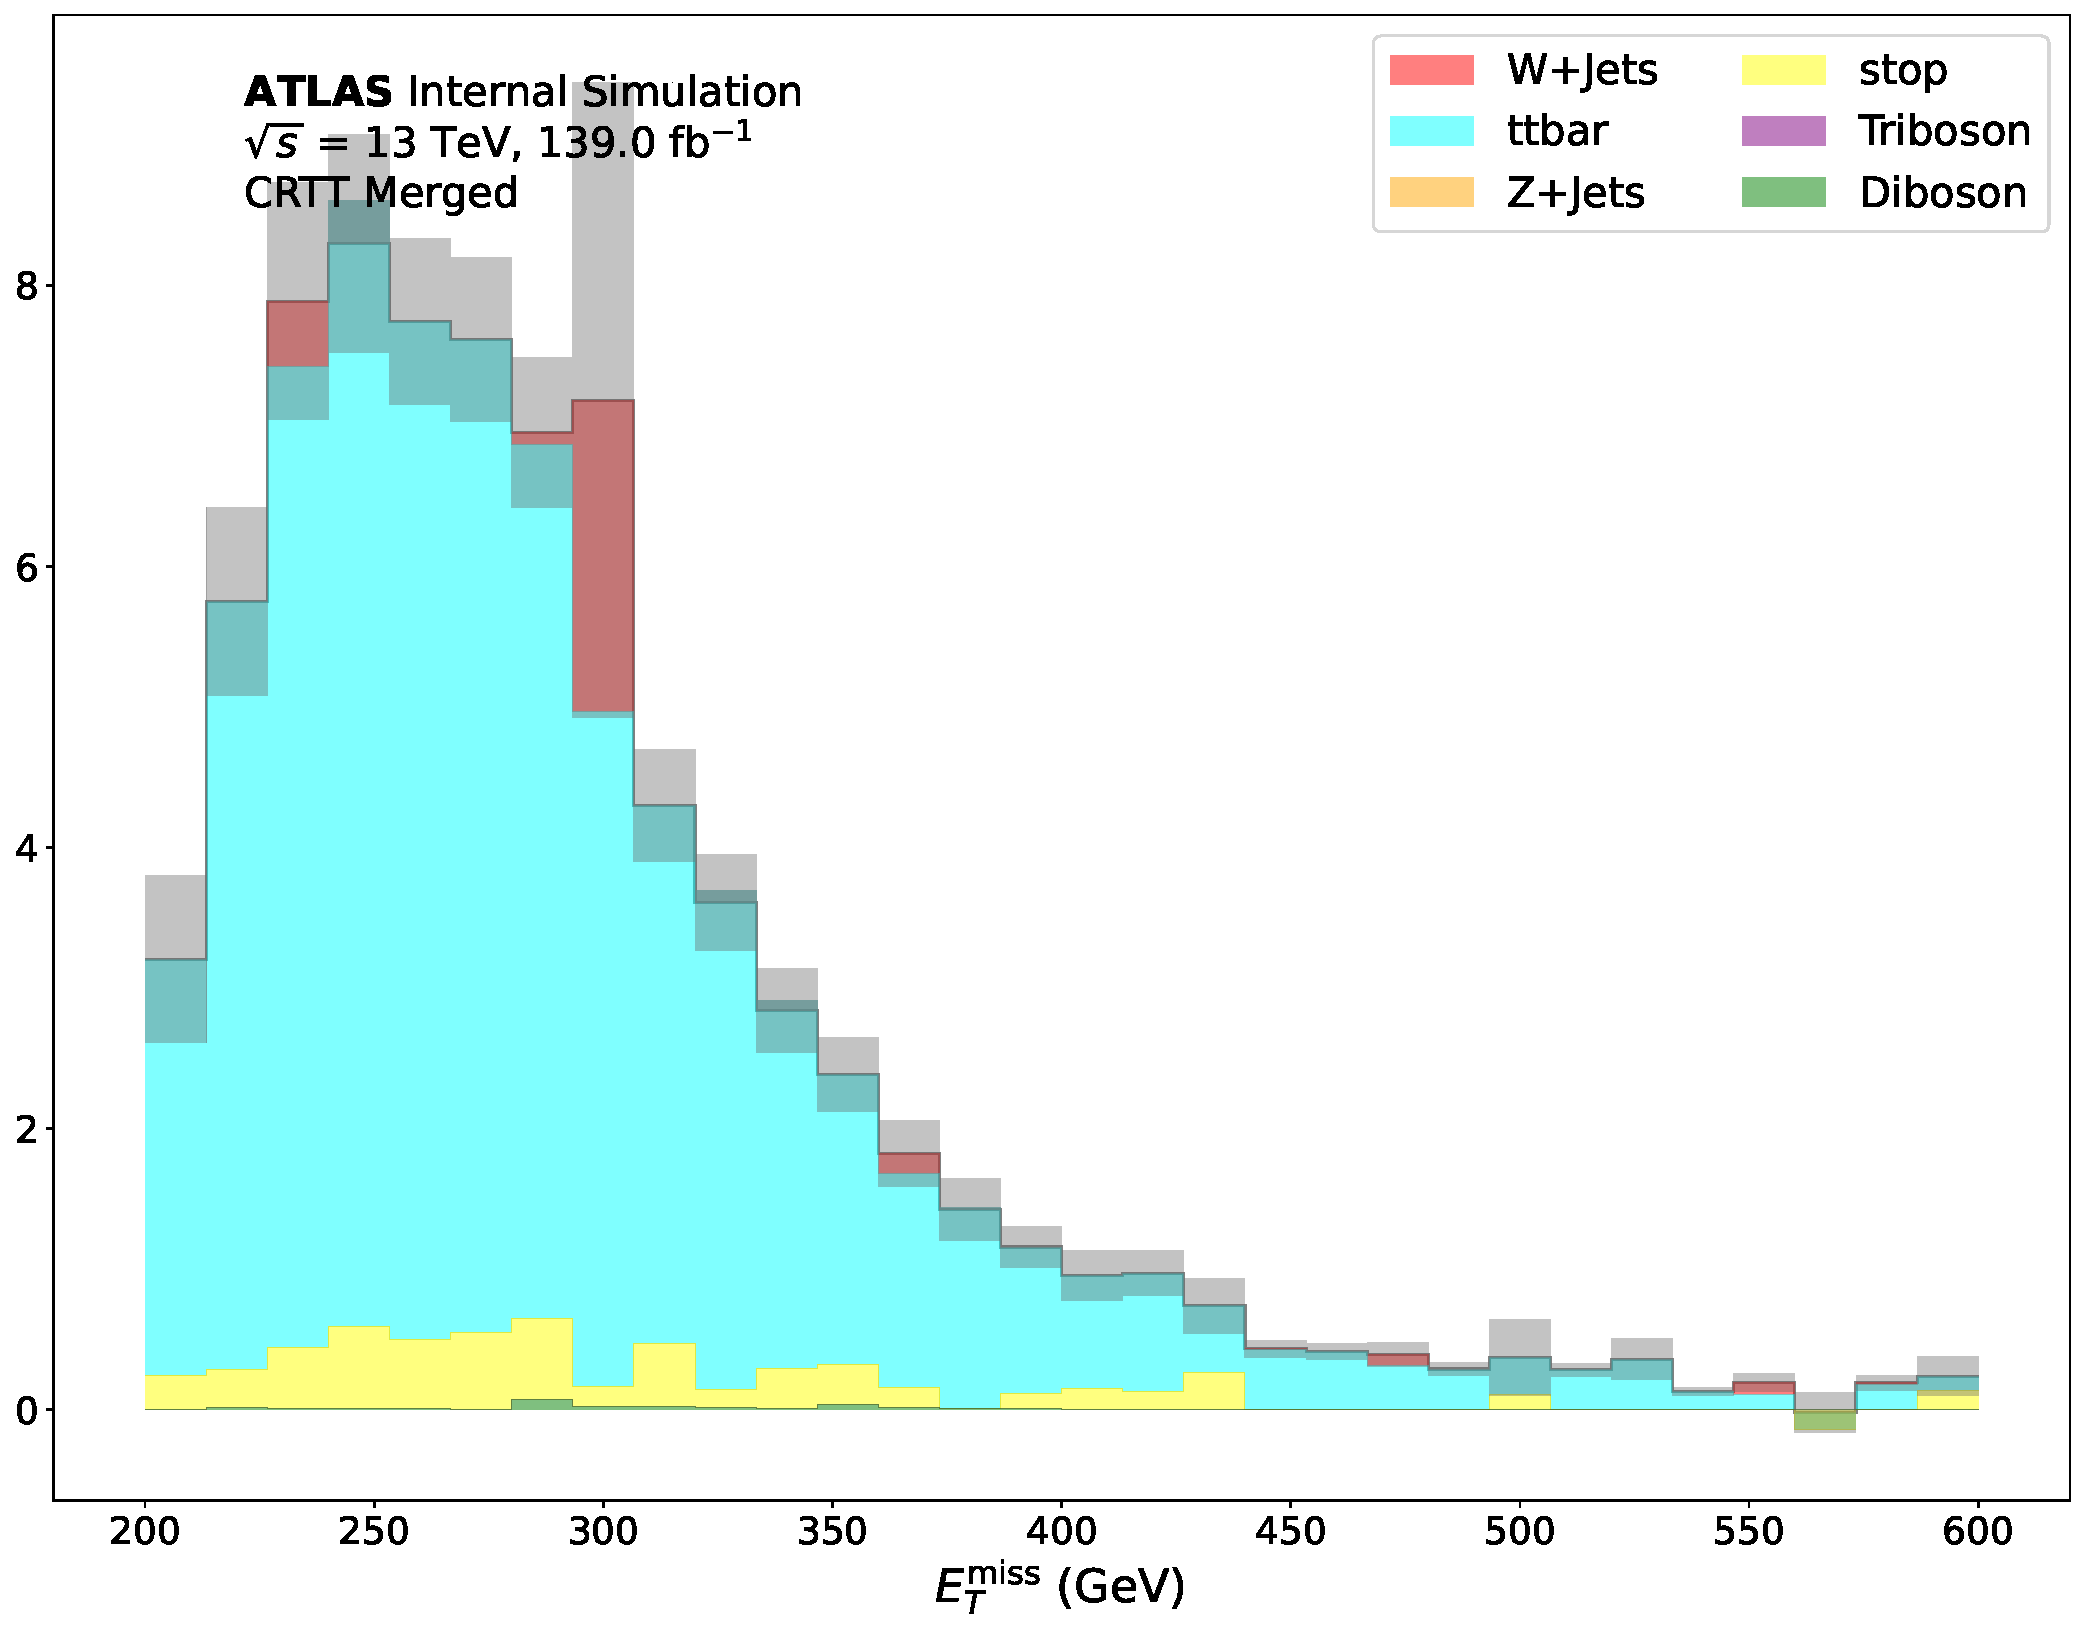
\includegraphics[width = 0.95\textwidth]{Figures/App_SR_CR_distributions/CRTT_Merged/MetTST_met_N_1.pdf}
     \caption{\met (merged \ttbar CR)}
     \end{subfigure}
     \caption{Comparison of N-1 distributions for kinematic variables of interest between the SR and the \ttbar CR in the merged category (continued).}
  \end{figure}


  \begin{figure}[htbp]
  \centering

     \begin{subfigure}{0.45\textwidth}
     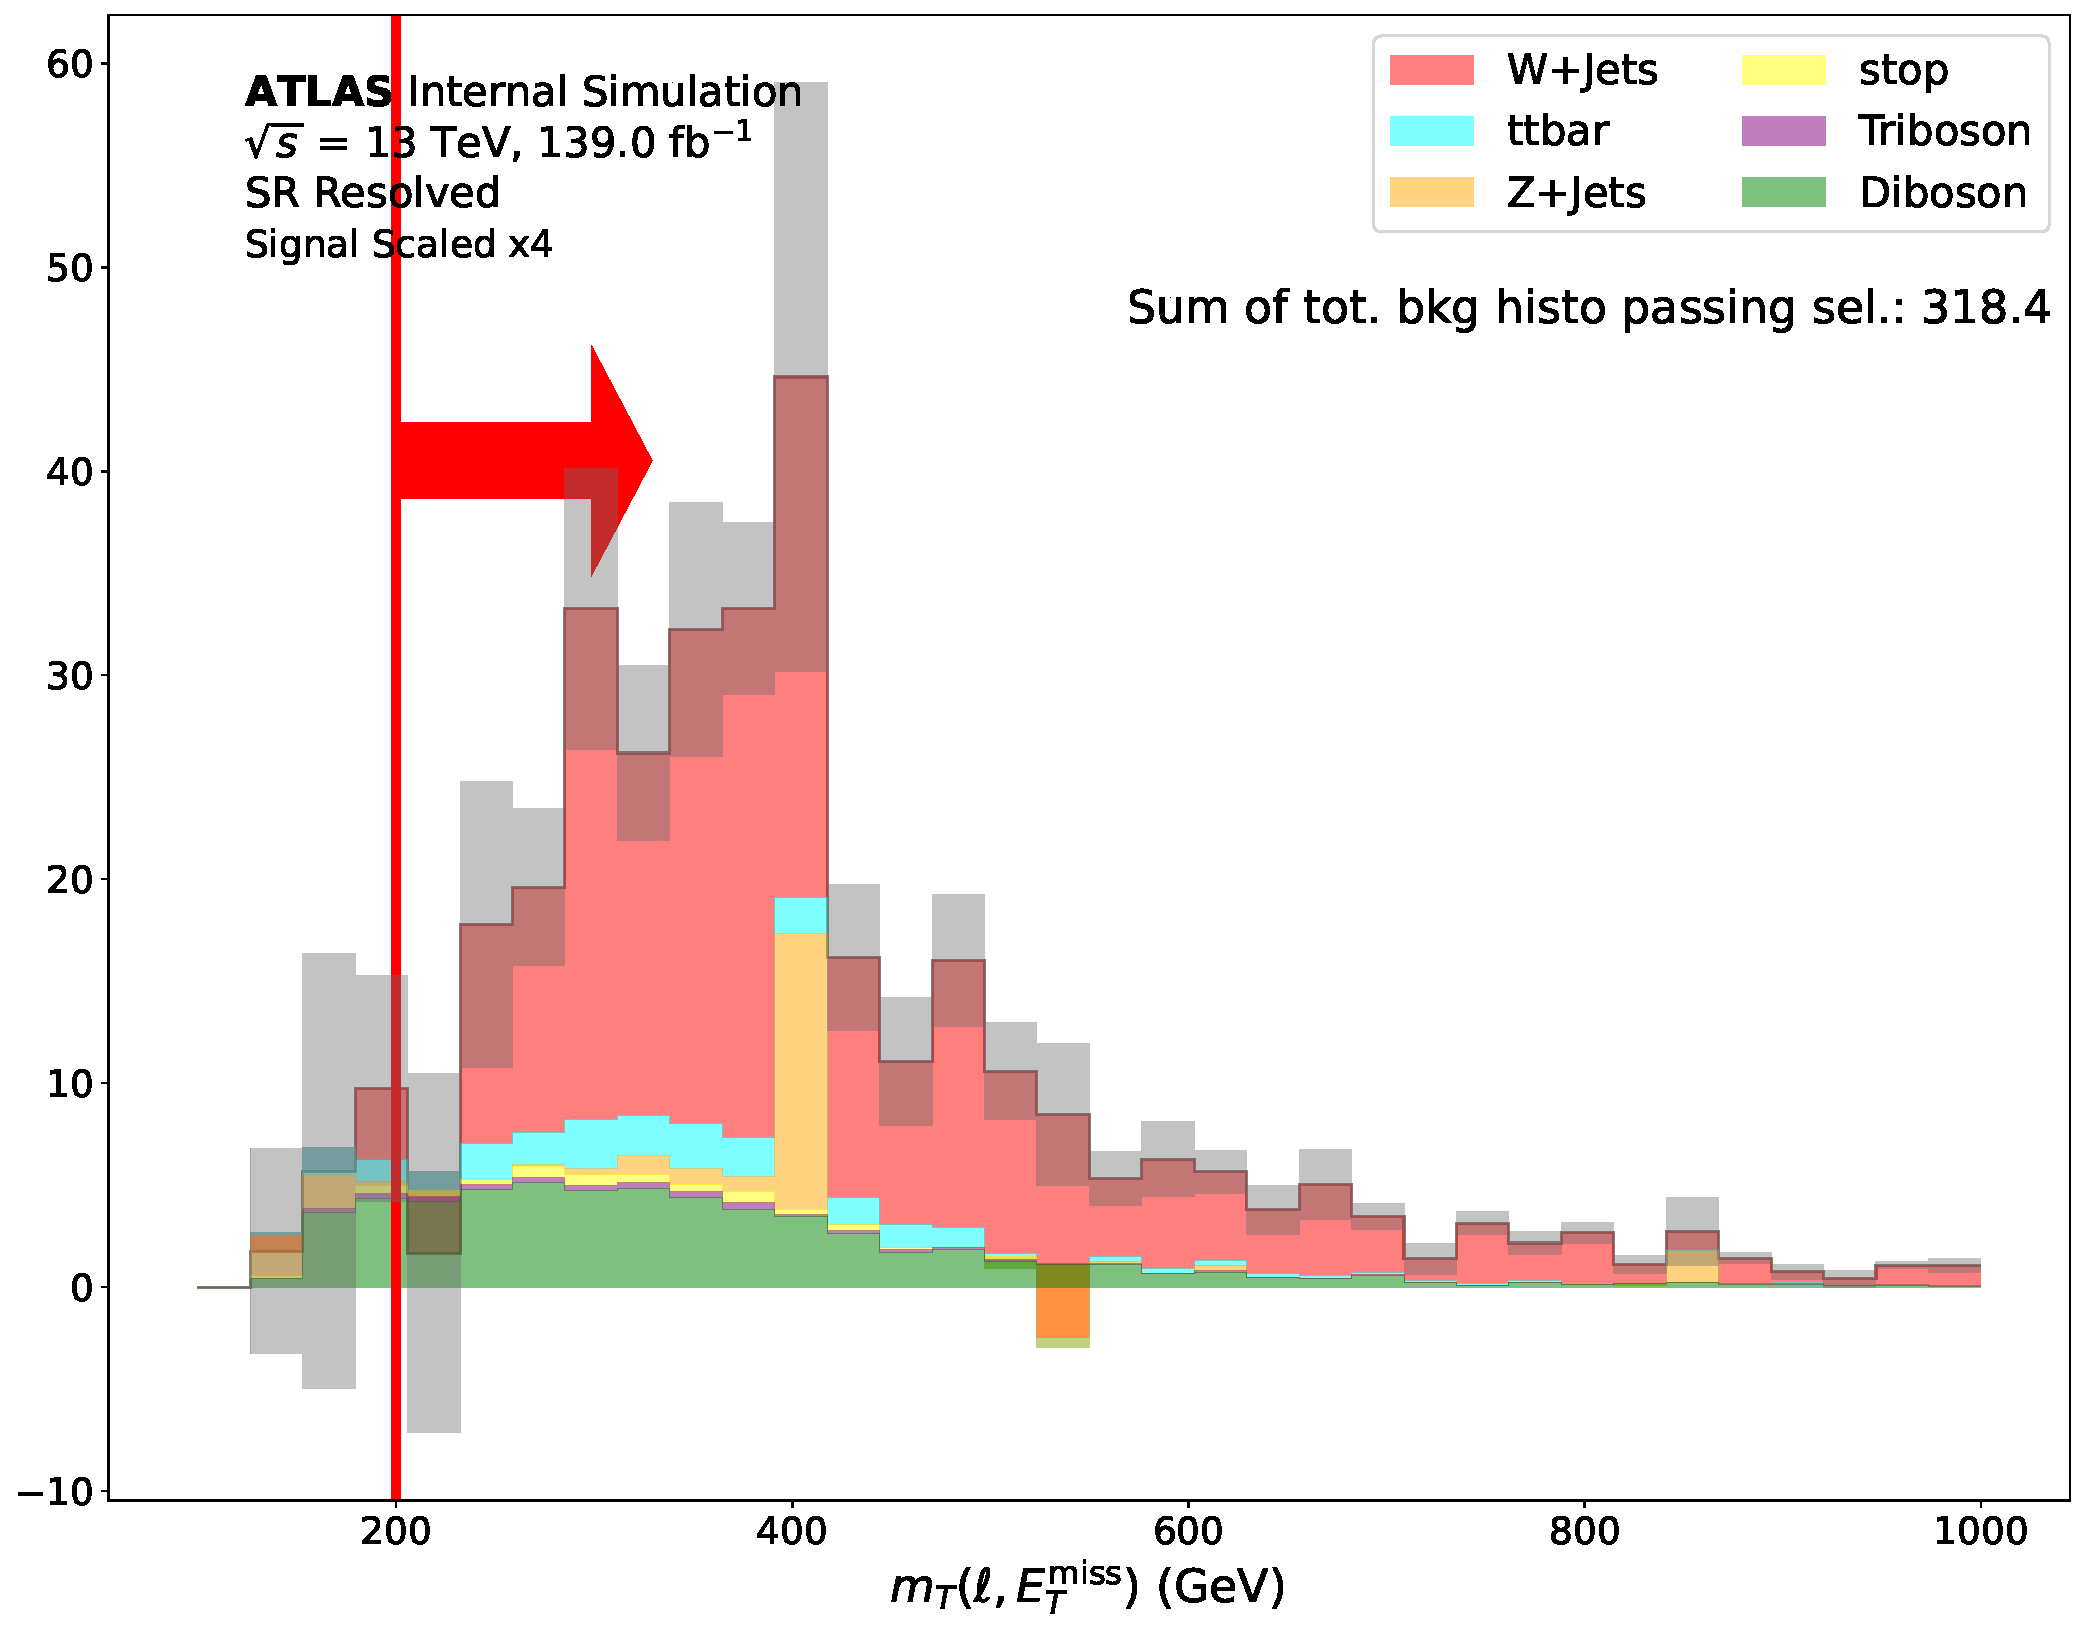
\includegraphics[width = 0.95\textwidth]{Figures/App_SR_CR_distributions/SR1L_Resolved/mT_lep_met_N_1.pdf}
    \caption{\mtlepmet (resolved SR)}
     \end{subfigure}
    \begin{subfigure}{0.45\textwidth}
     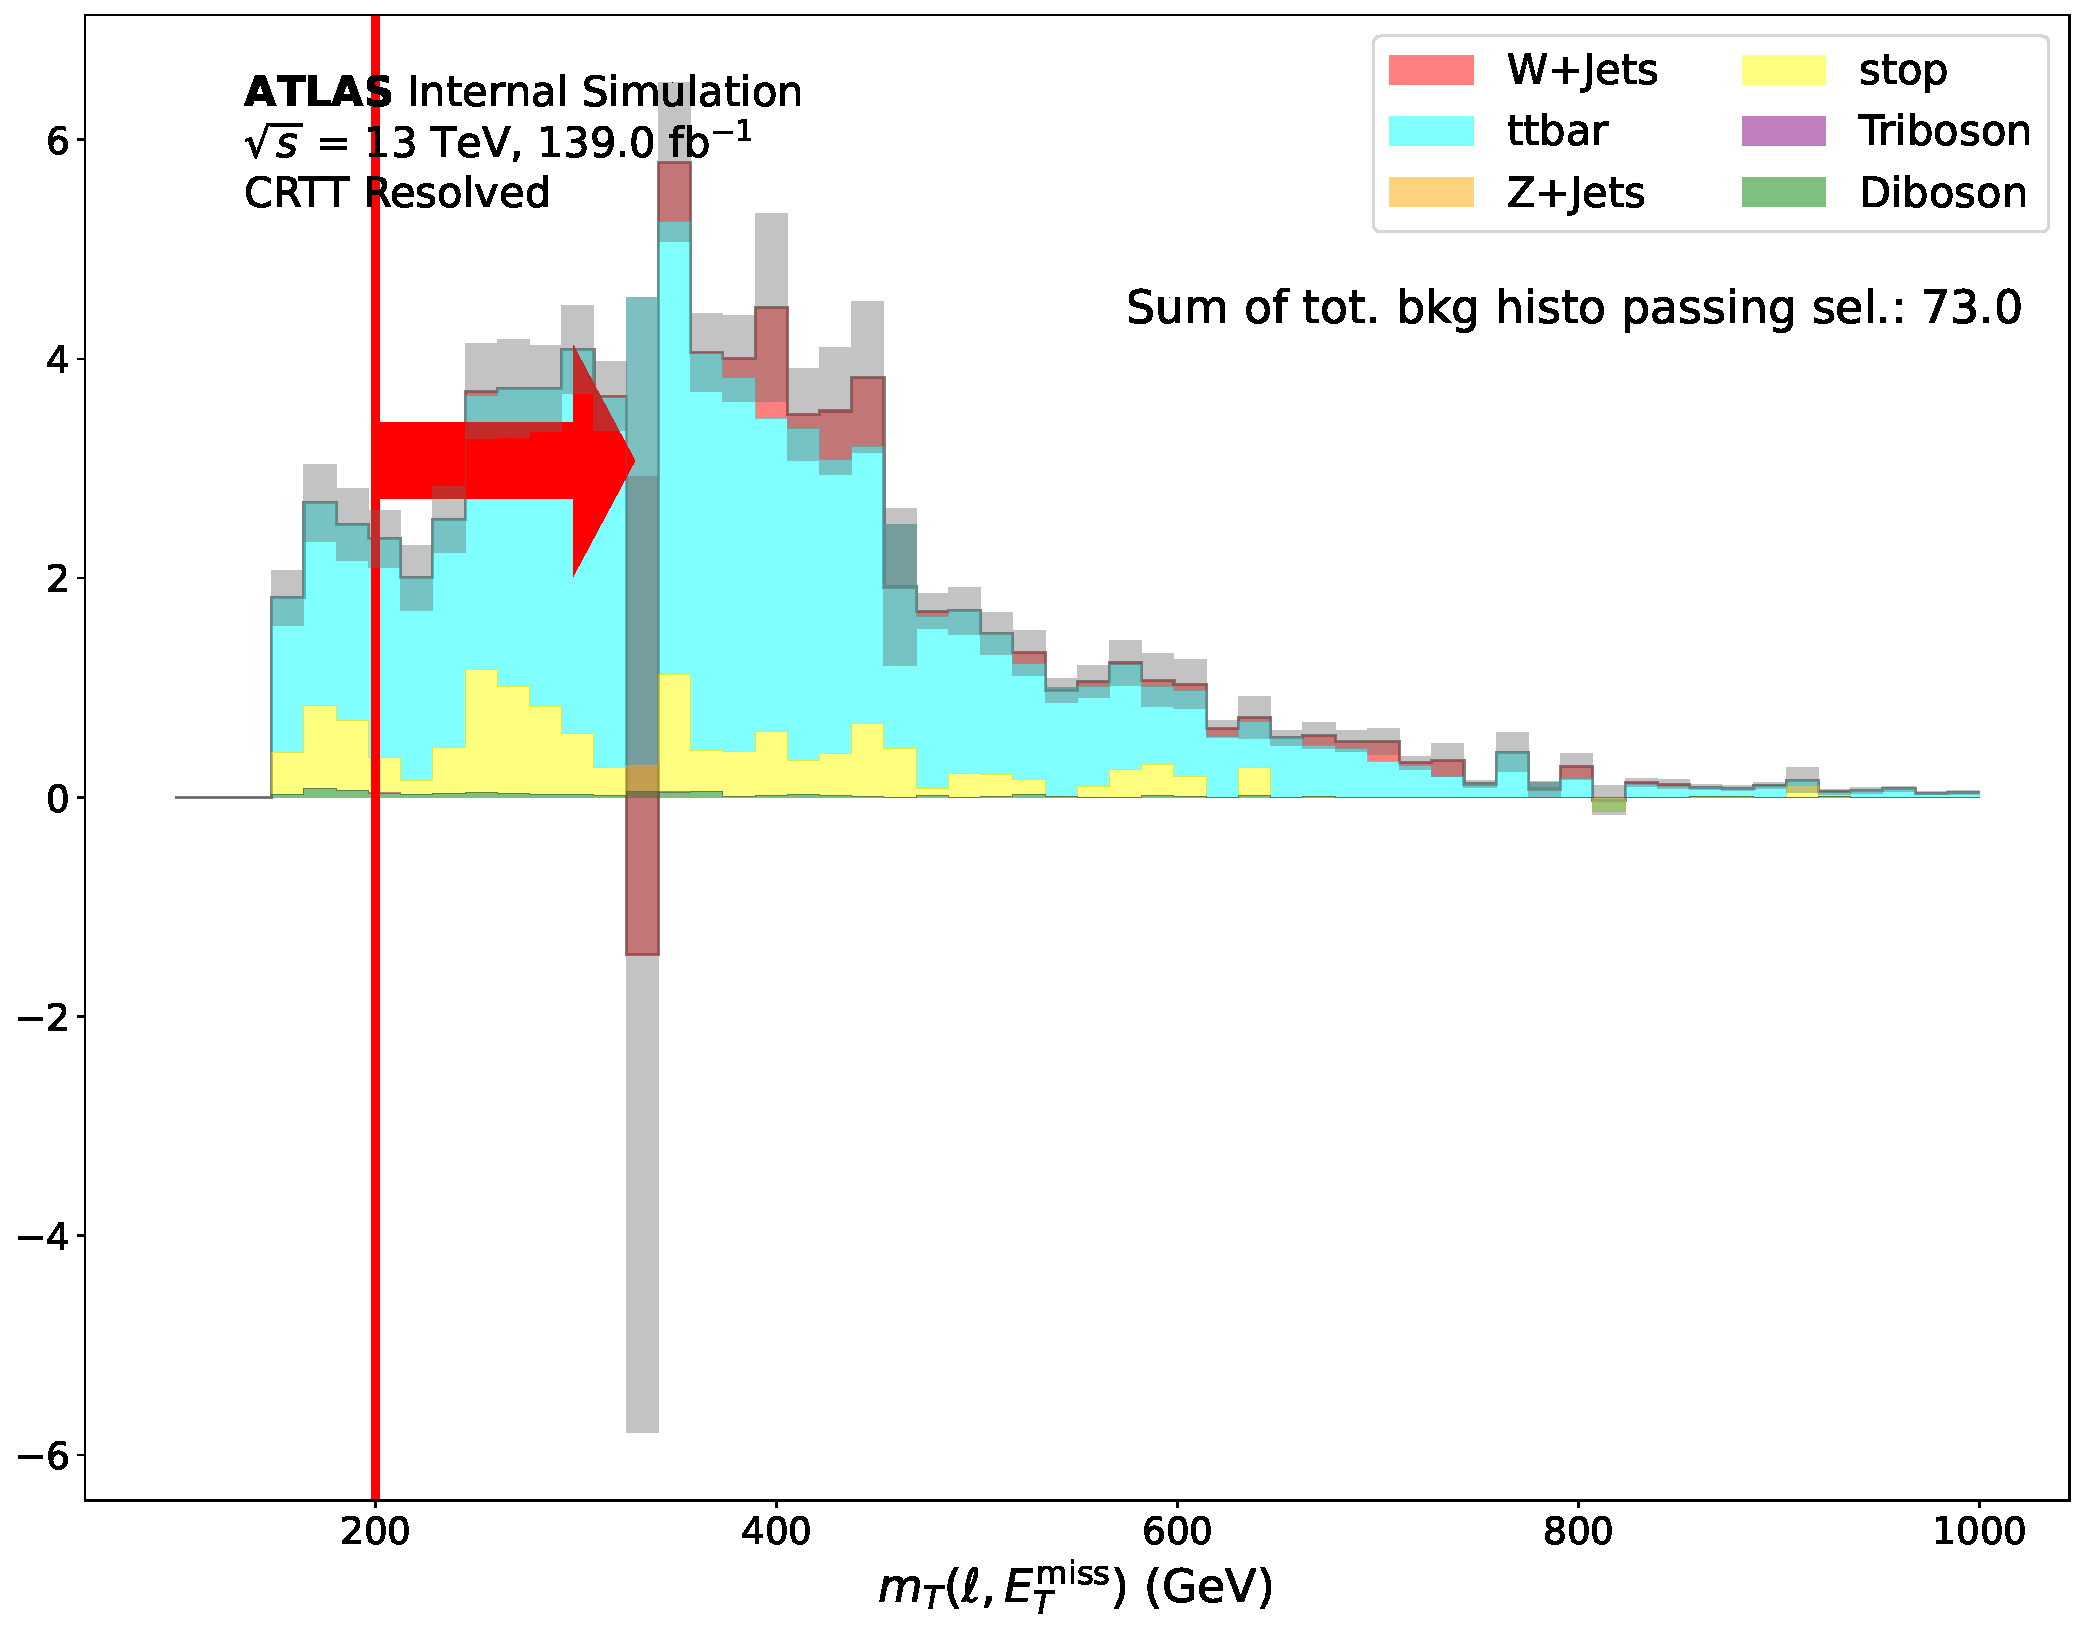
\includegraphics[width = 0.95\textwidth]{Figures/App_SR_CR_distributions/CRTT_Resolved/mT_lep_met_N_1.pdf}
     \caption{\mtlepmet (resolved \ttbar CR)}
     \end{subfigure}

  \begin{subfigure}{0.45\textwidth}
     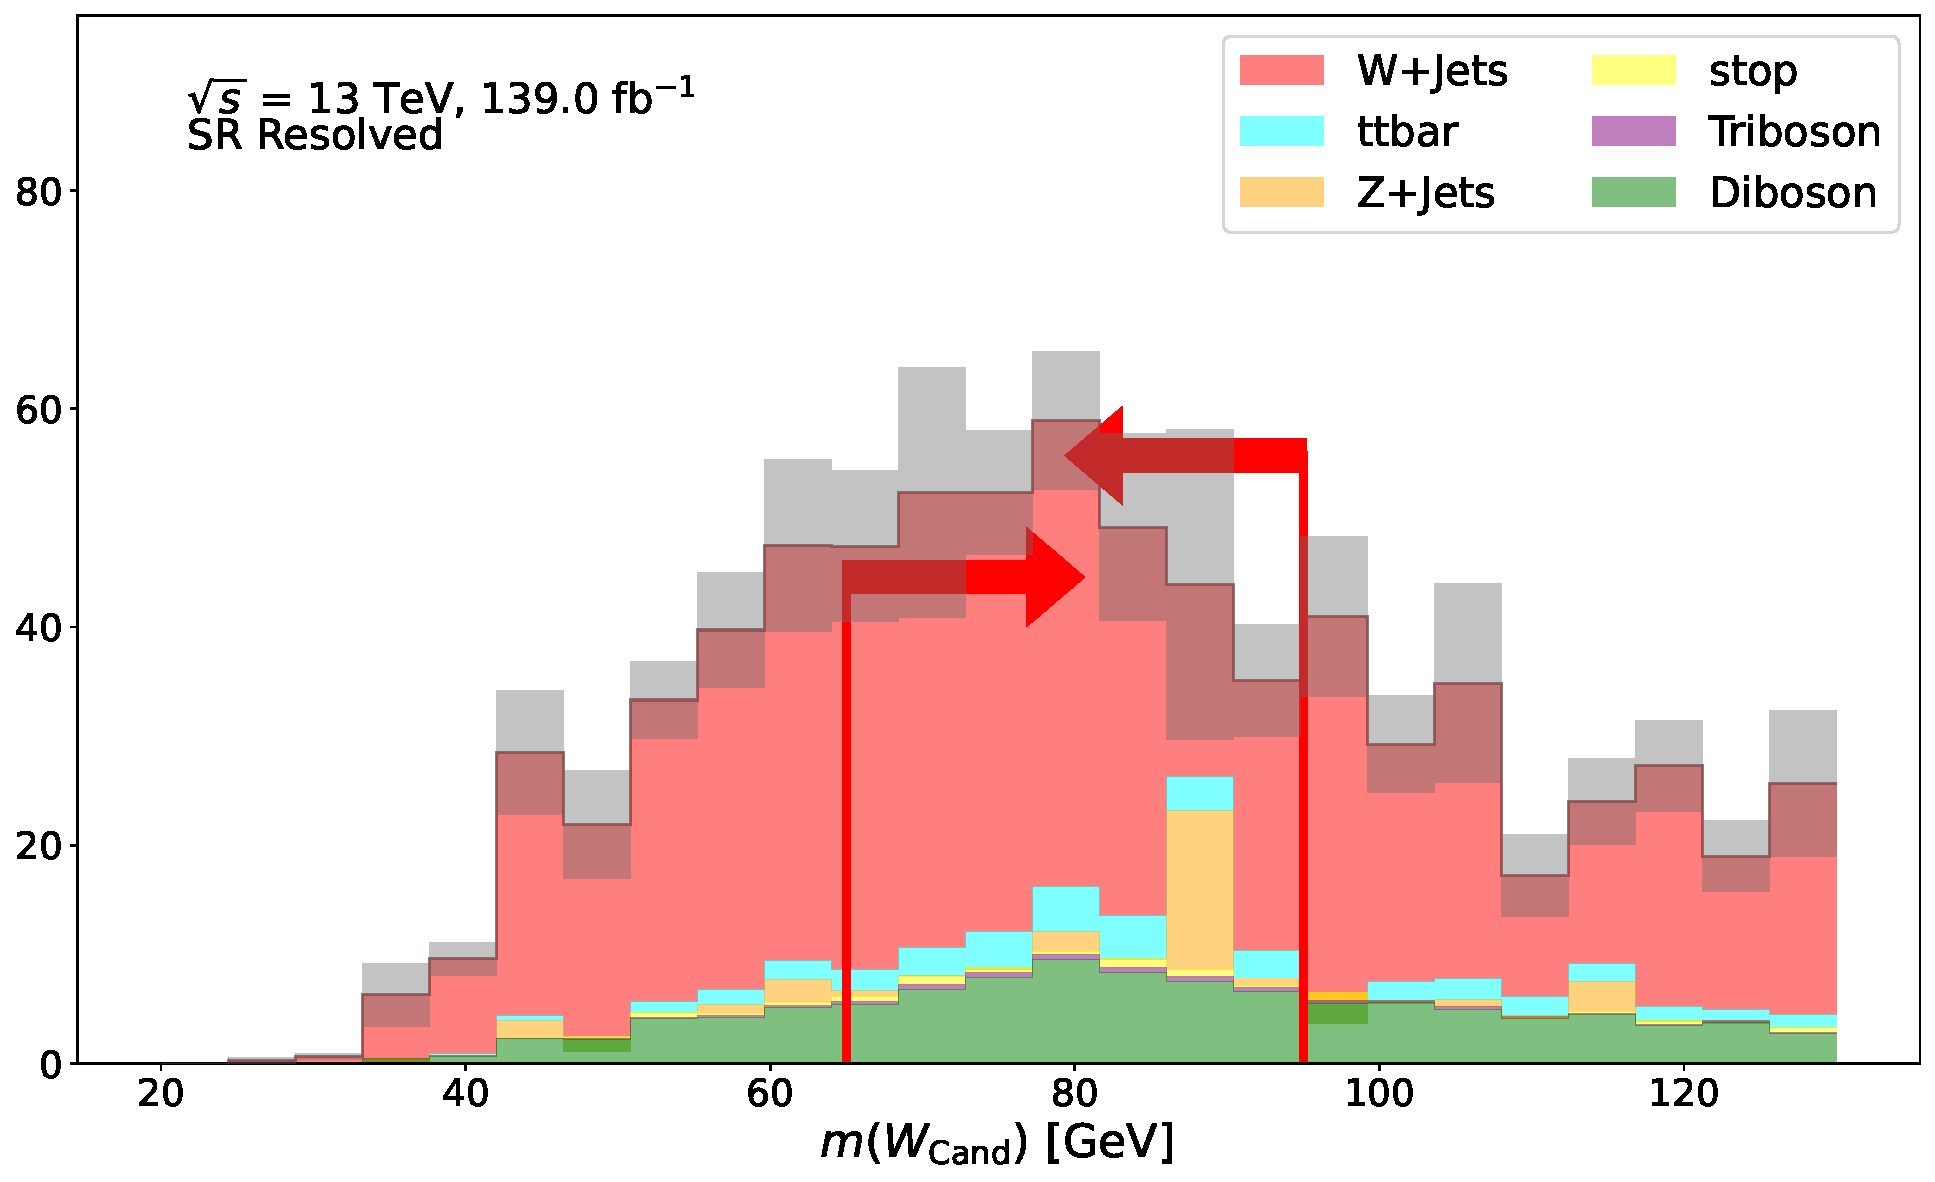
\includegraphics[width = 0.95\textwidth]{Figures/App_SR_CR_distributions/SR1L_Resolved/WCand_m_N_1.pdf}
    \caption{\Wcandm (resolved SR)}
     \end{subfigure}
    \begin{subfigure}{0.45\textwidth}
     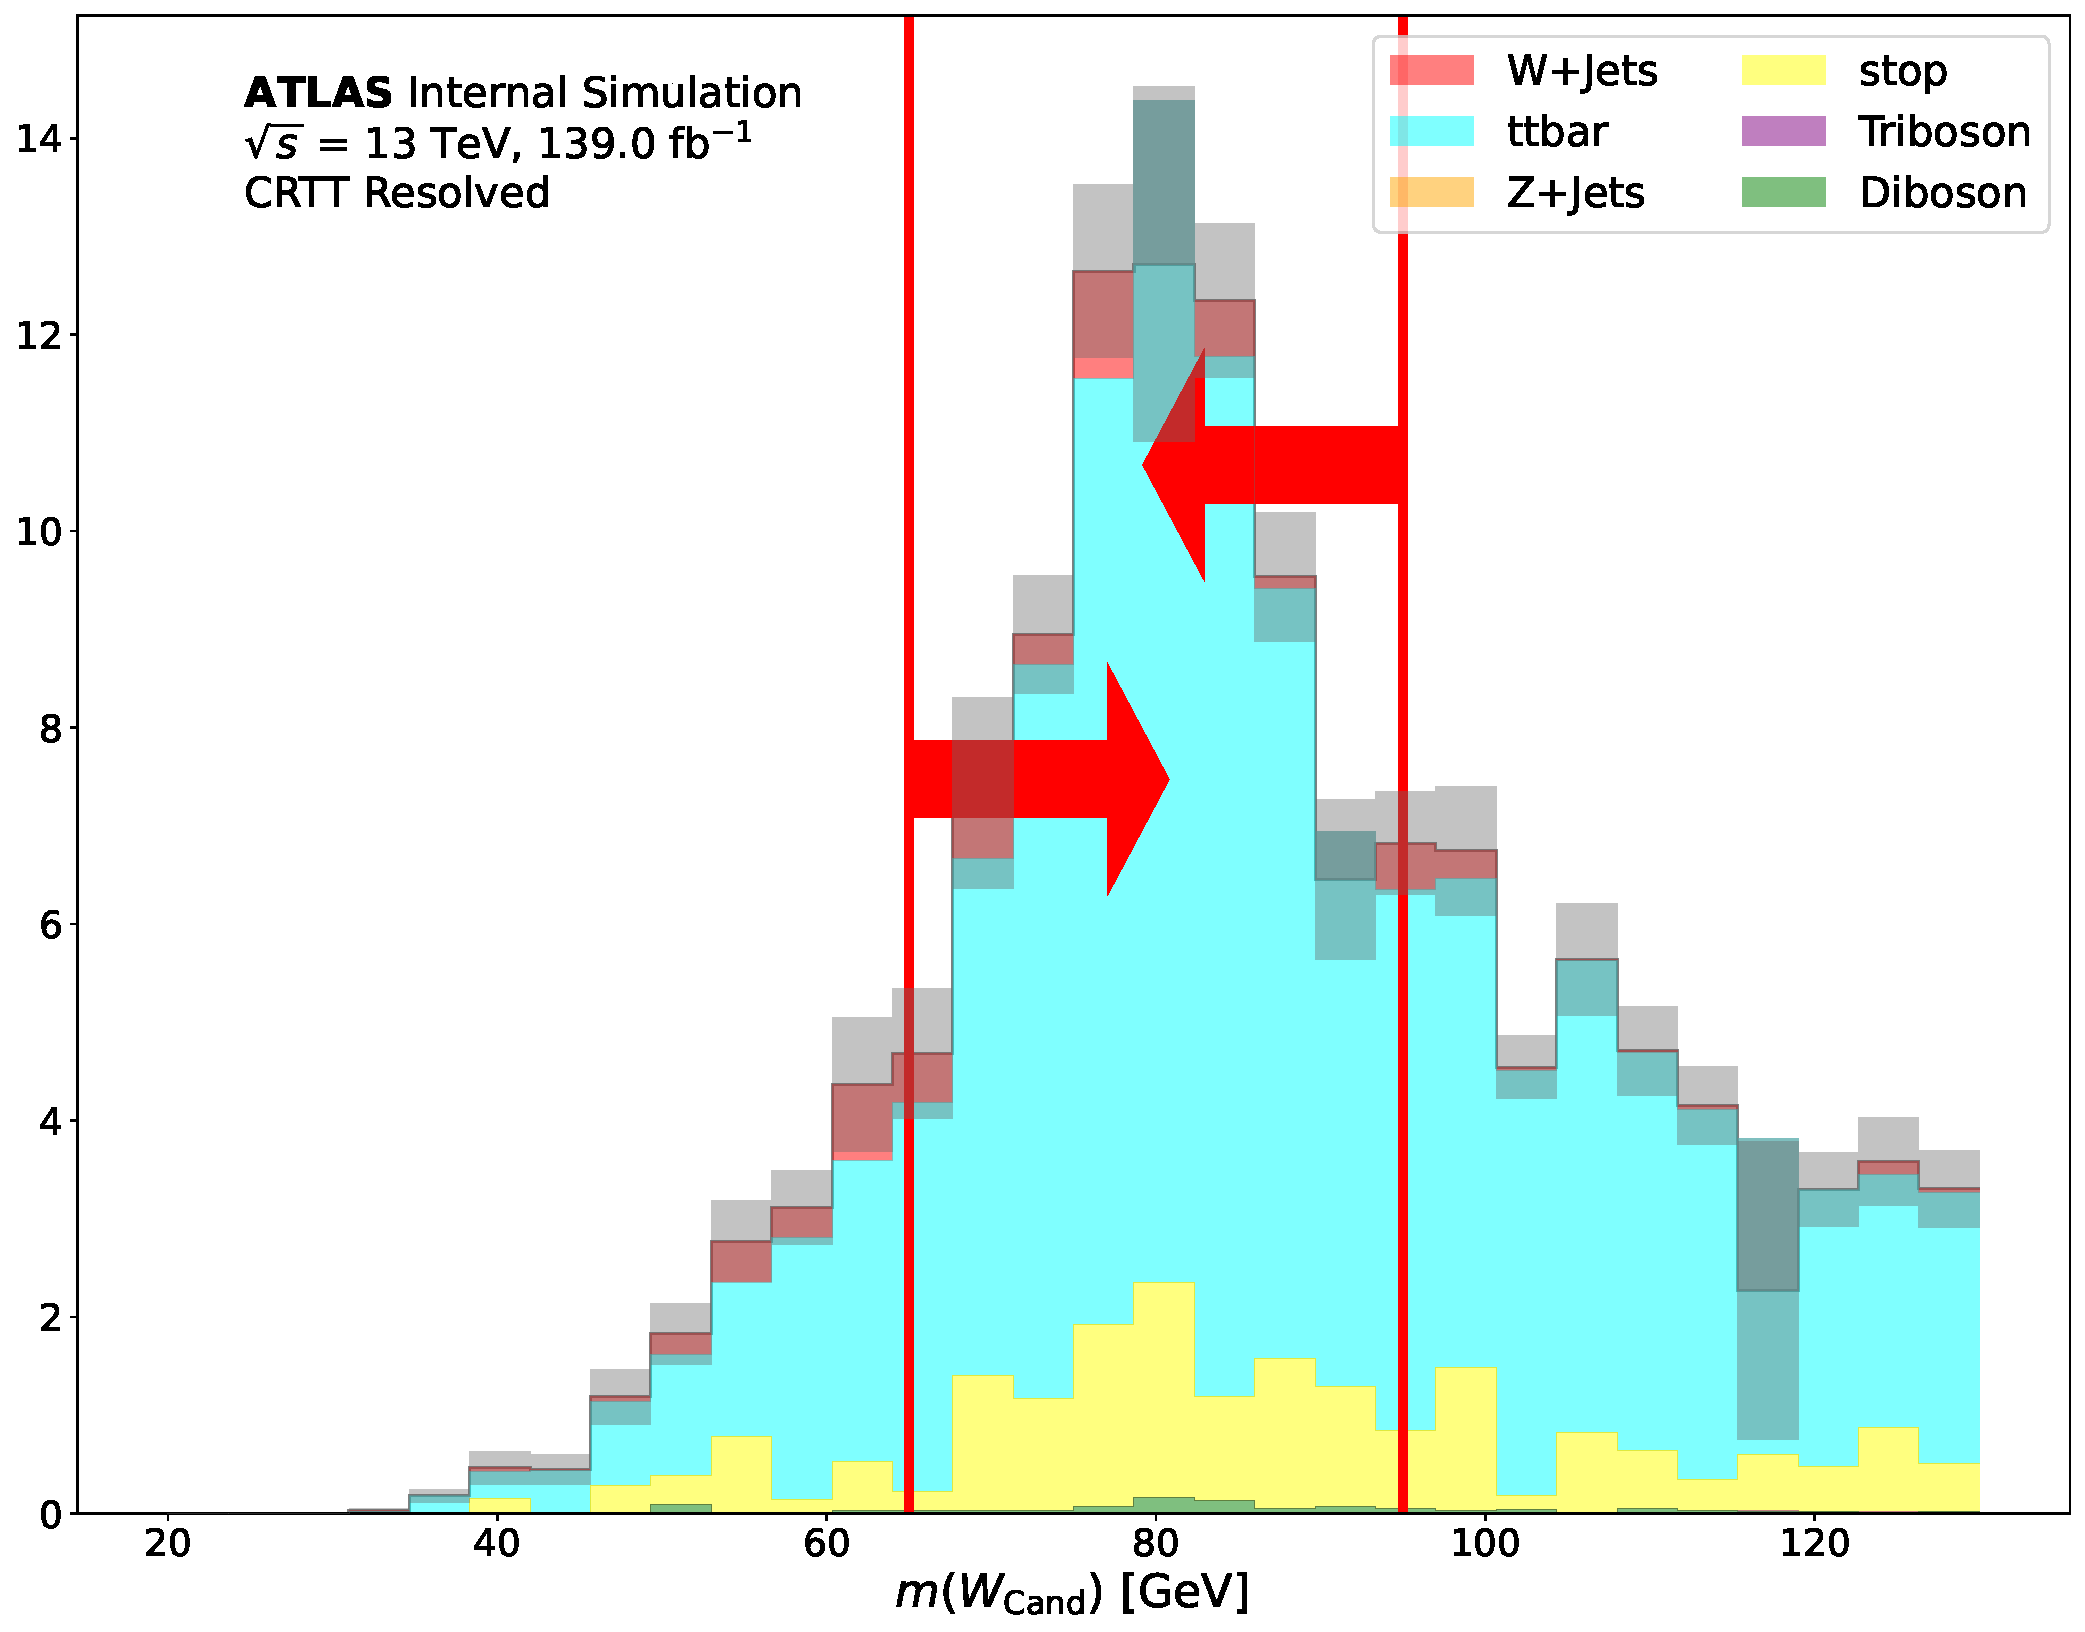
\includegraphics[width = 0.95\textwidth]{Figures/App_SR_CR_distributions/CRTT_Resolved/WCand_m_N_1.pdf}
     \caption{\Wcandm (resolved \ttbar CR)}
     \end{subfigure}

  \begin{subfigure}{0.45\textwidth}
     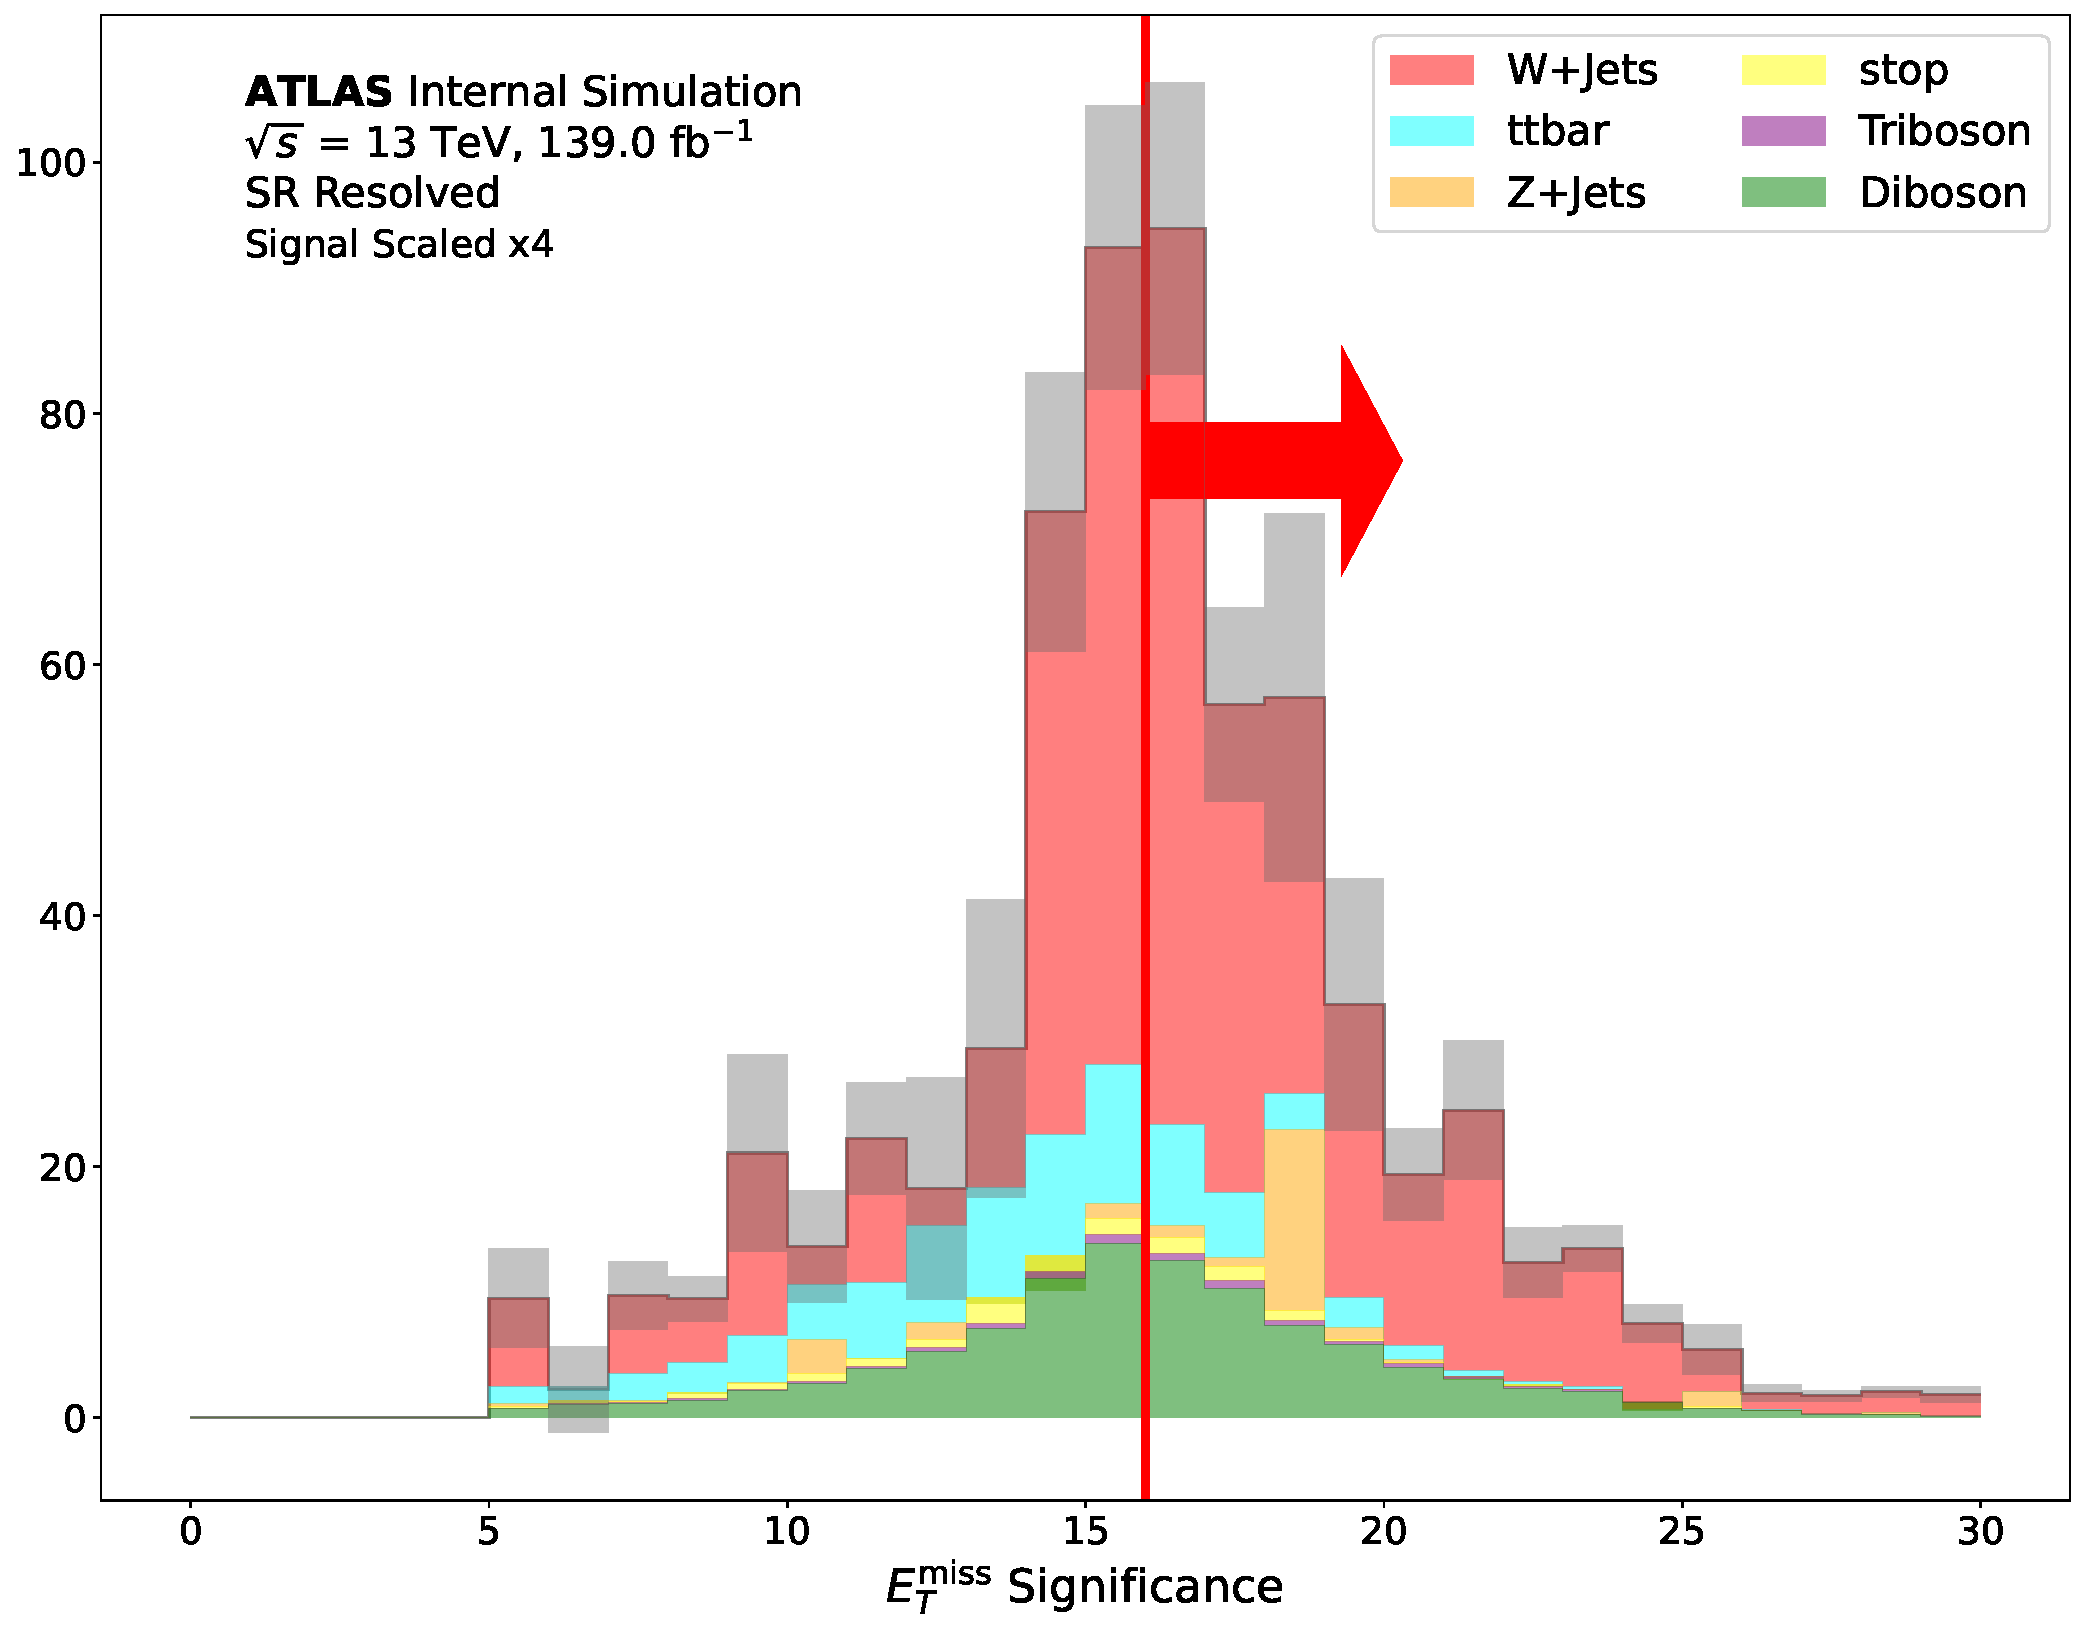
\includegraphics[width = 0.95\textwidth]{Figures/App_SR_CR_distributions/SR1L_Resolved/MetTST_Significance_N_1.pdf}
    \caption{\metsig (resolved SR)}
     \end{subfigure}
    \begin{subfigure}{0.45\textwidth}
     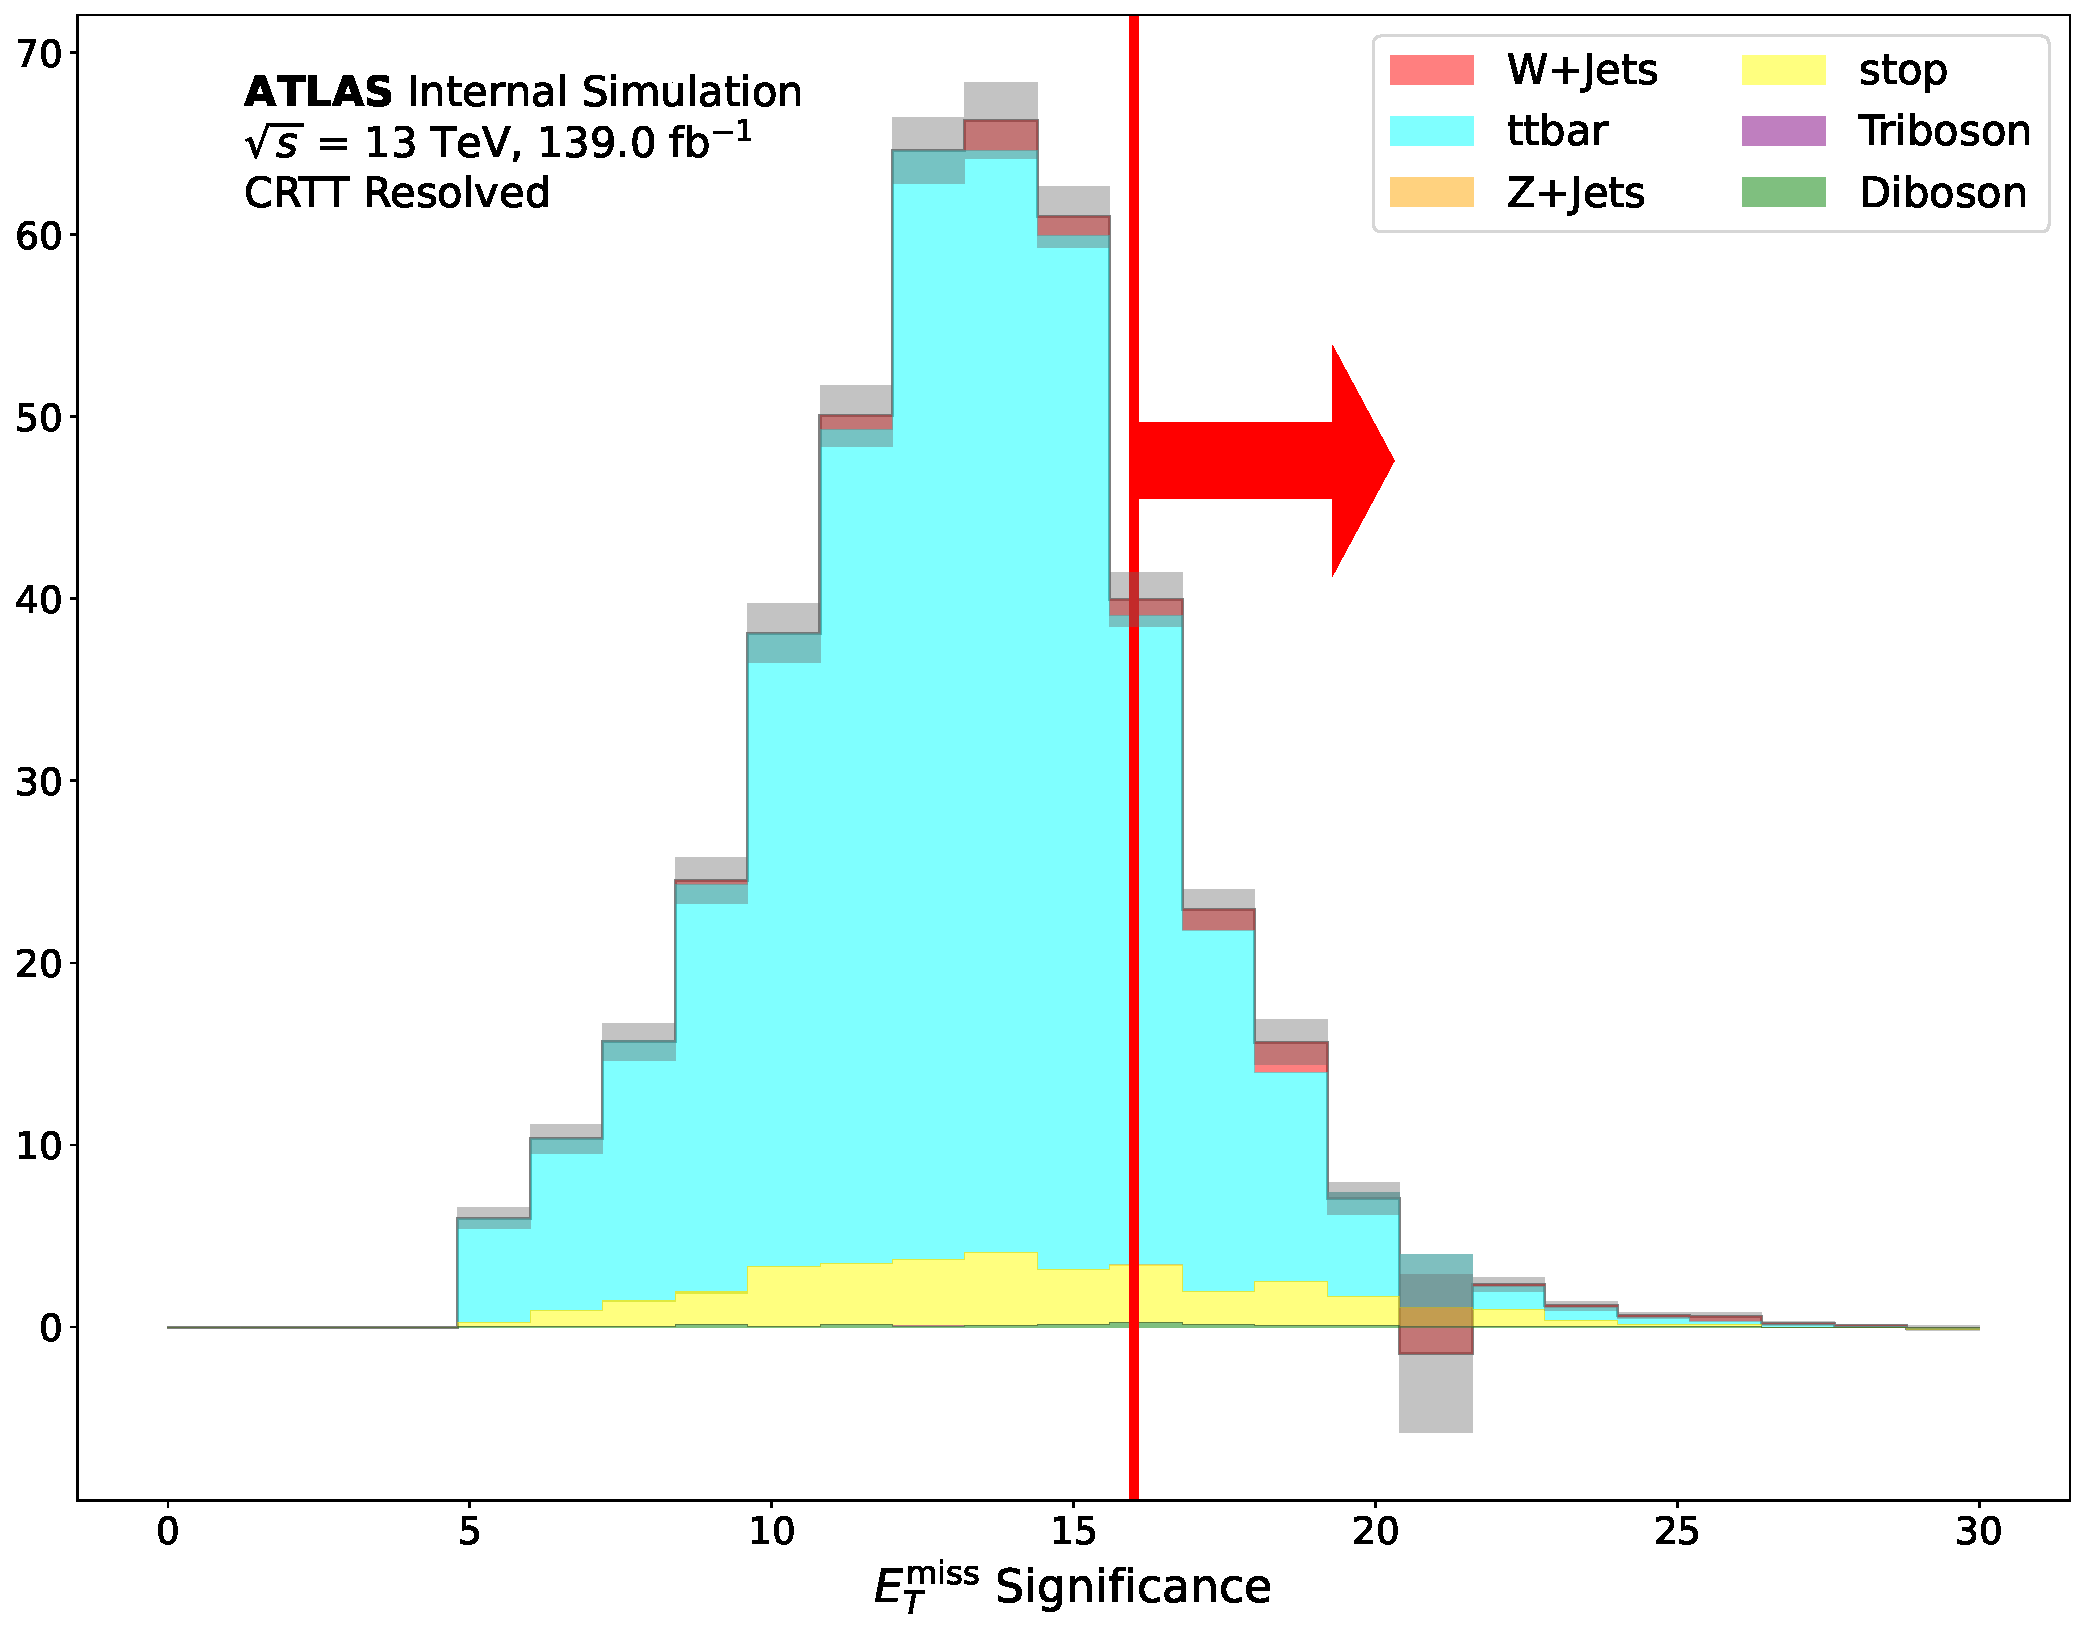
\includegraphics[width = 0.95\textwidth]{Figures/App_SR_CR_distributions/CRTT_Resolved/MetTST_Significance_N_1.pdf}
     \caption{\metsig (resolved \ttbar CR)}
     \end{subfigure}
     \caption{Comparison of N-1 distributions for kinematic variables of interest between the SR and the \ttbar CR in the merged category. Grey bands show statistical uncertainty on the background estimate.}
     \end{figure}

    \begin{figure}[htbp]\ContinuedFloat
   \begin{subfigure}{0.45\textwidth}
     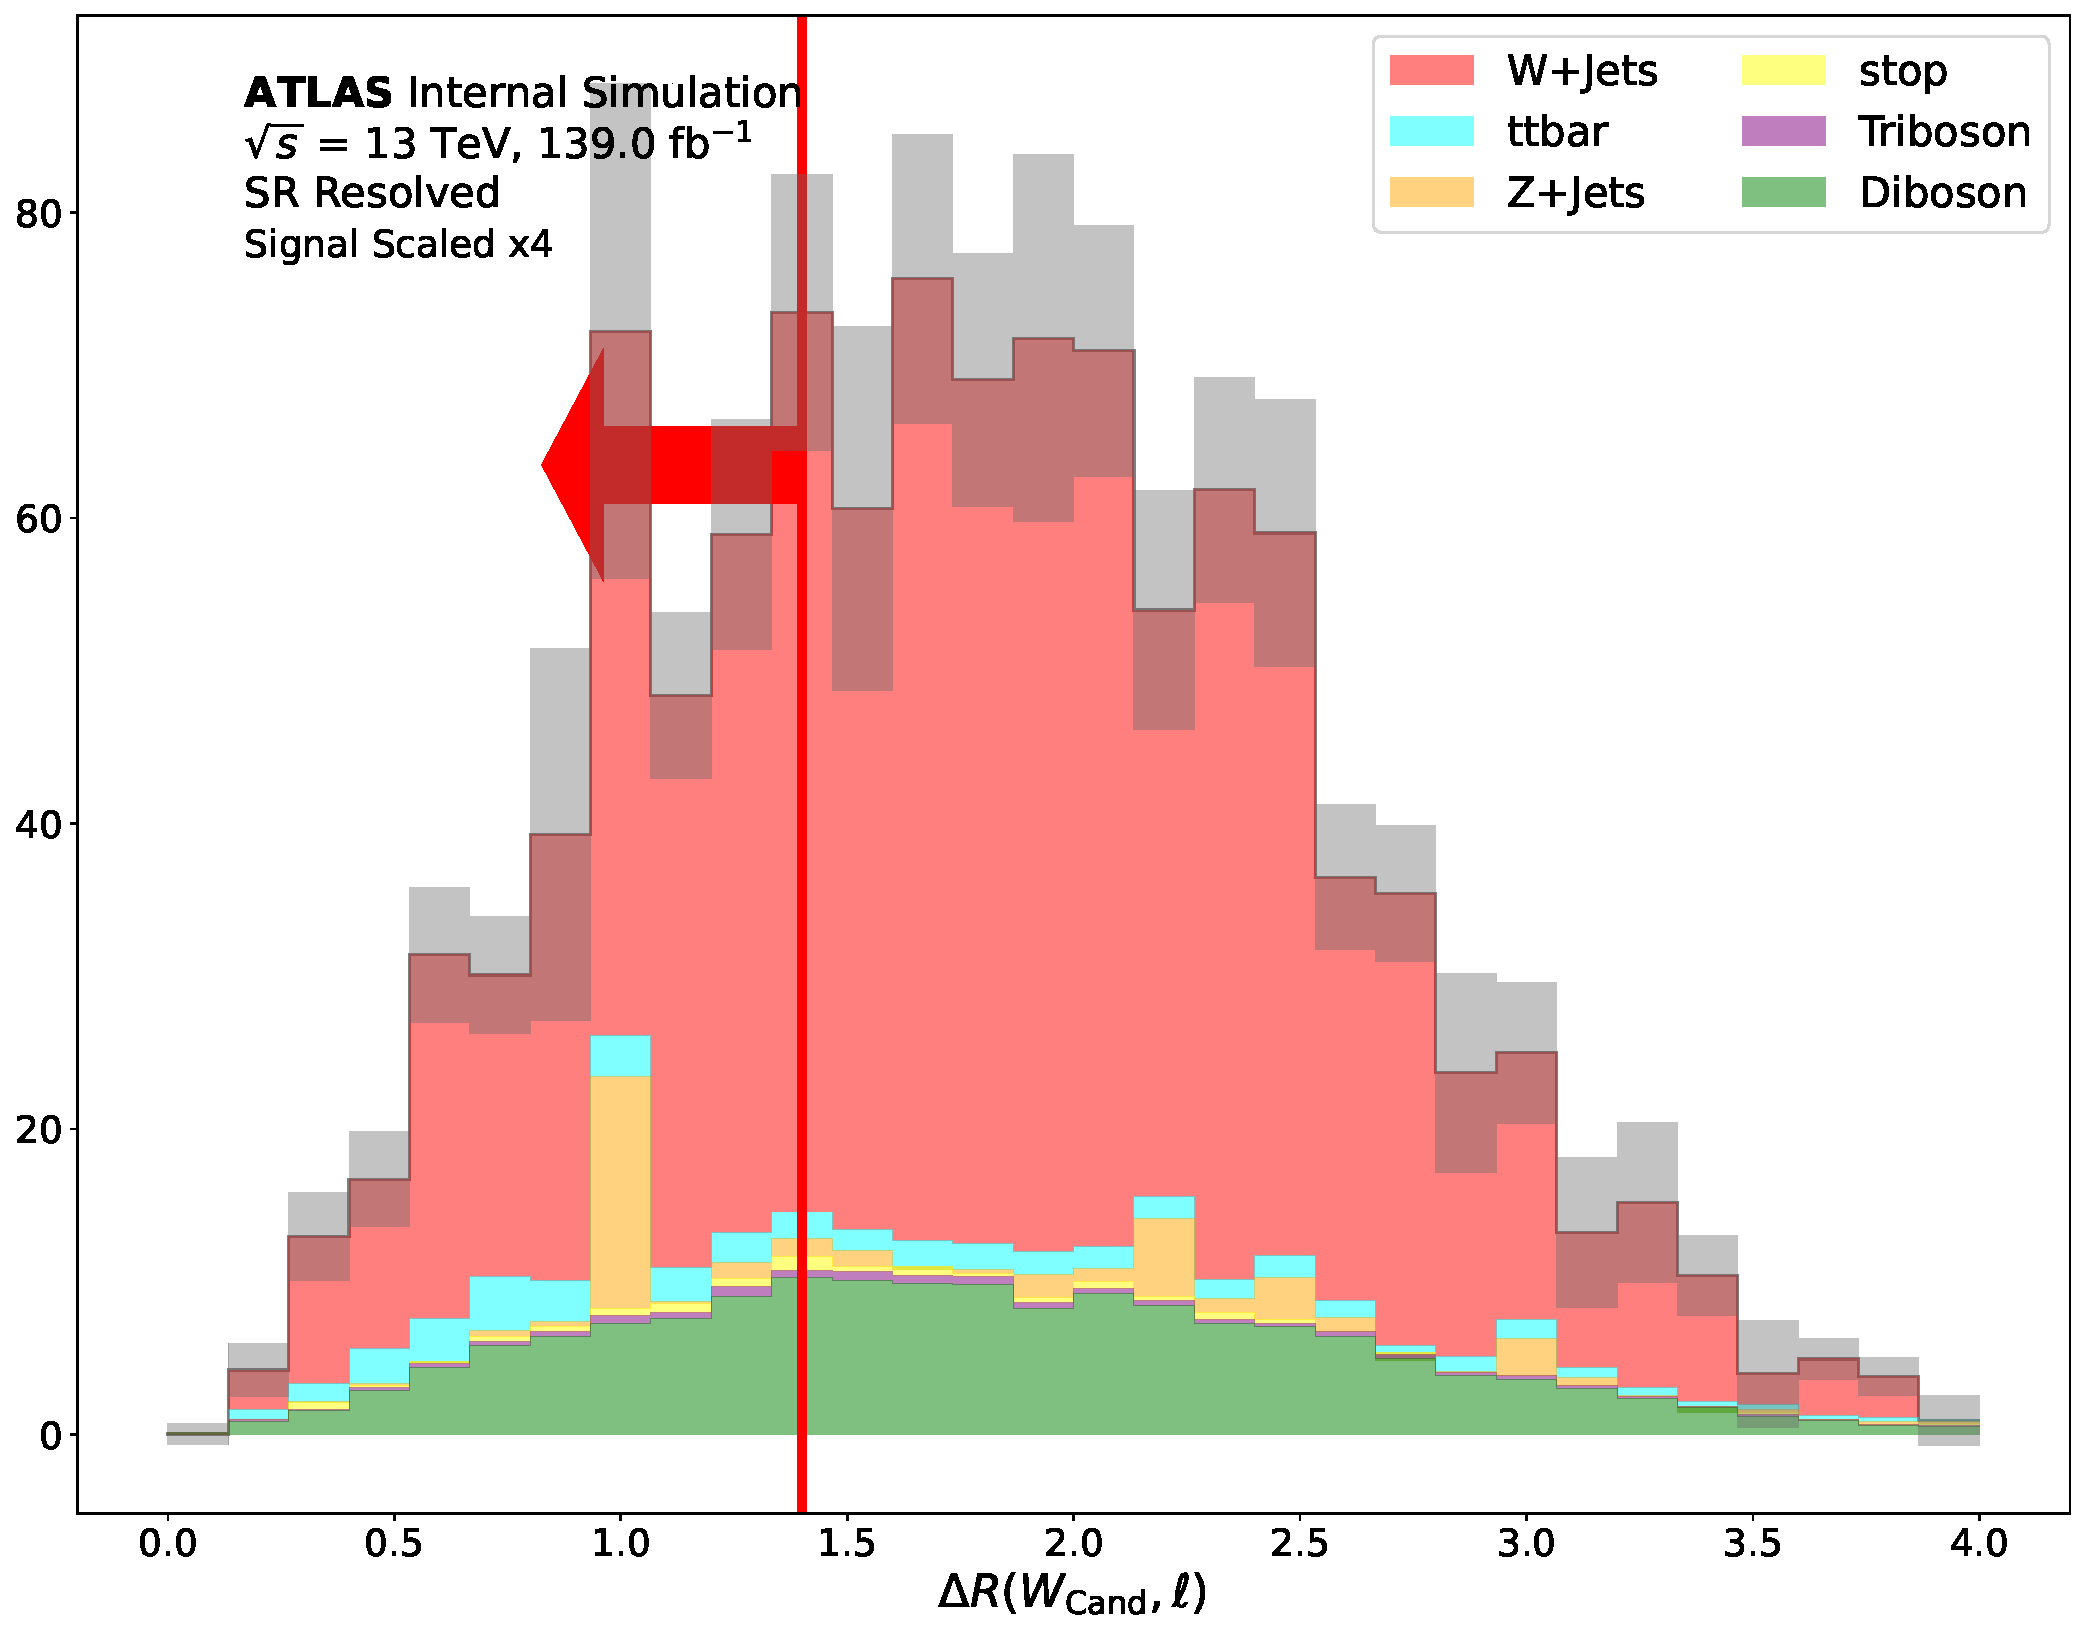
\includegraphics[width = 0.95\textwidth]{Figures/App_SR_CR_distributions/SR1L_Resolved/dRWl_N_1.pdf}
    \caption{\drWl (resolved SR)}
     \end{subfigure}
    \begin{subfigure}{0.45\textwidth}
     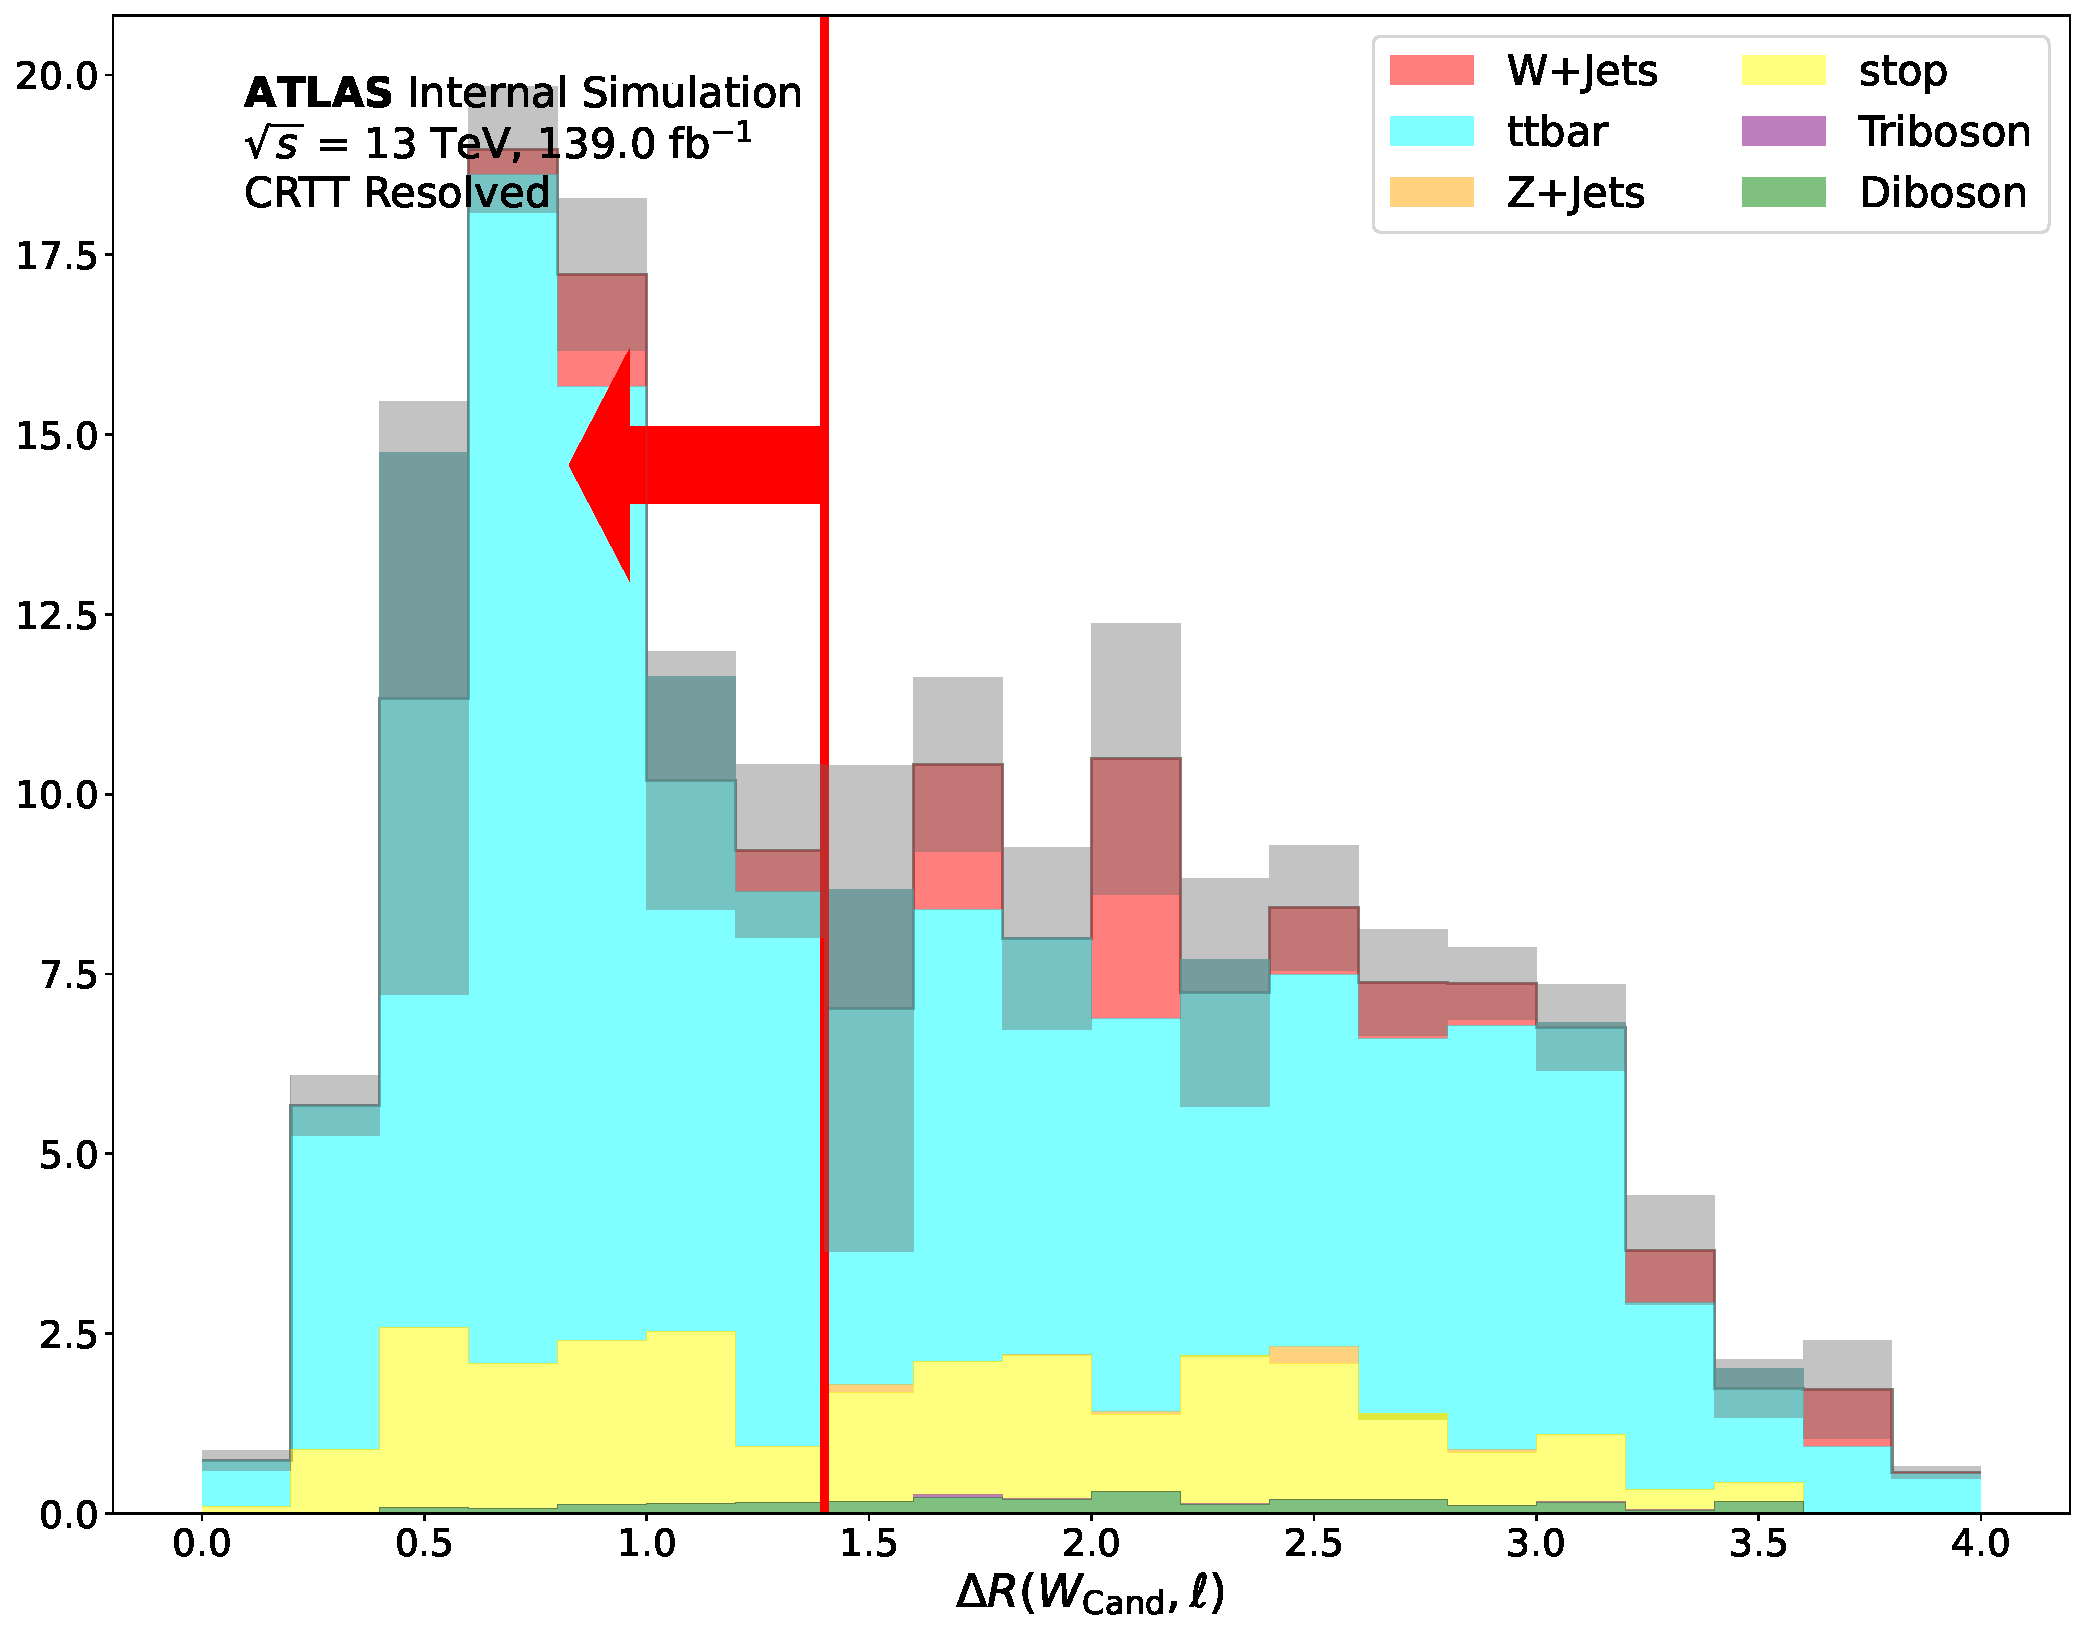
\includegraphics[width = 0.95\textwidth]{Figures/App_SR_CR_distributions/CRTT_Resolved/dRWl_N_1.pdf}
     \caption{\drWl (resolved \ttbar CR)}
     \end{subfigure}

    \begin{subfigure}{0.45\textwidth}
     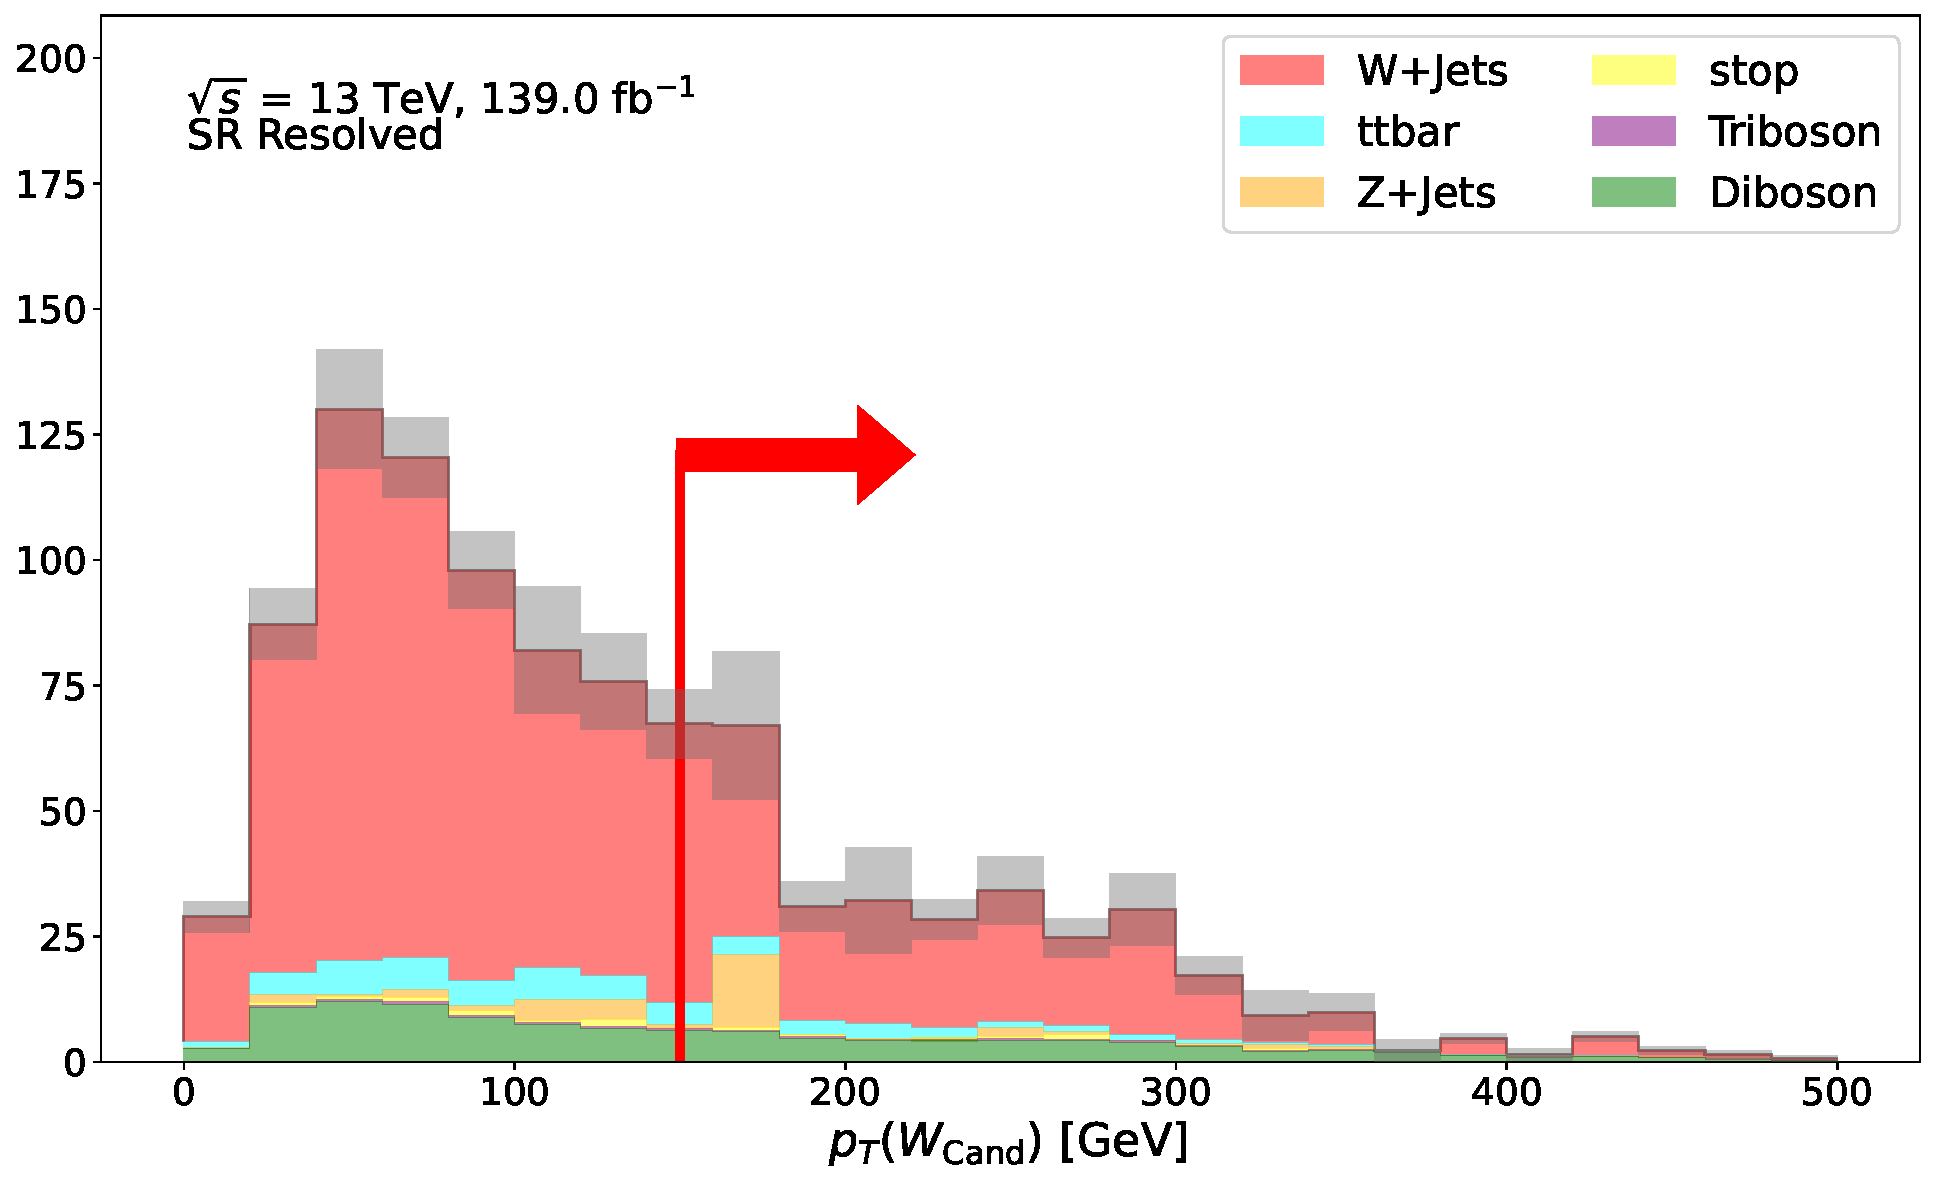
\includegraphics[width = 0.95\textwidth]{Figures/App_SR_CR_distributions/SR1L_Resolved/WCand_pt_N_1.pdf}
    \caption{\Wcandpt (resolved SR)}
     \end{subfigure}
    \begin{subfigure}{0.45\textwidth}
     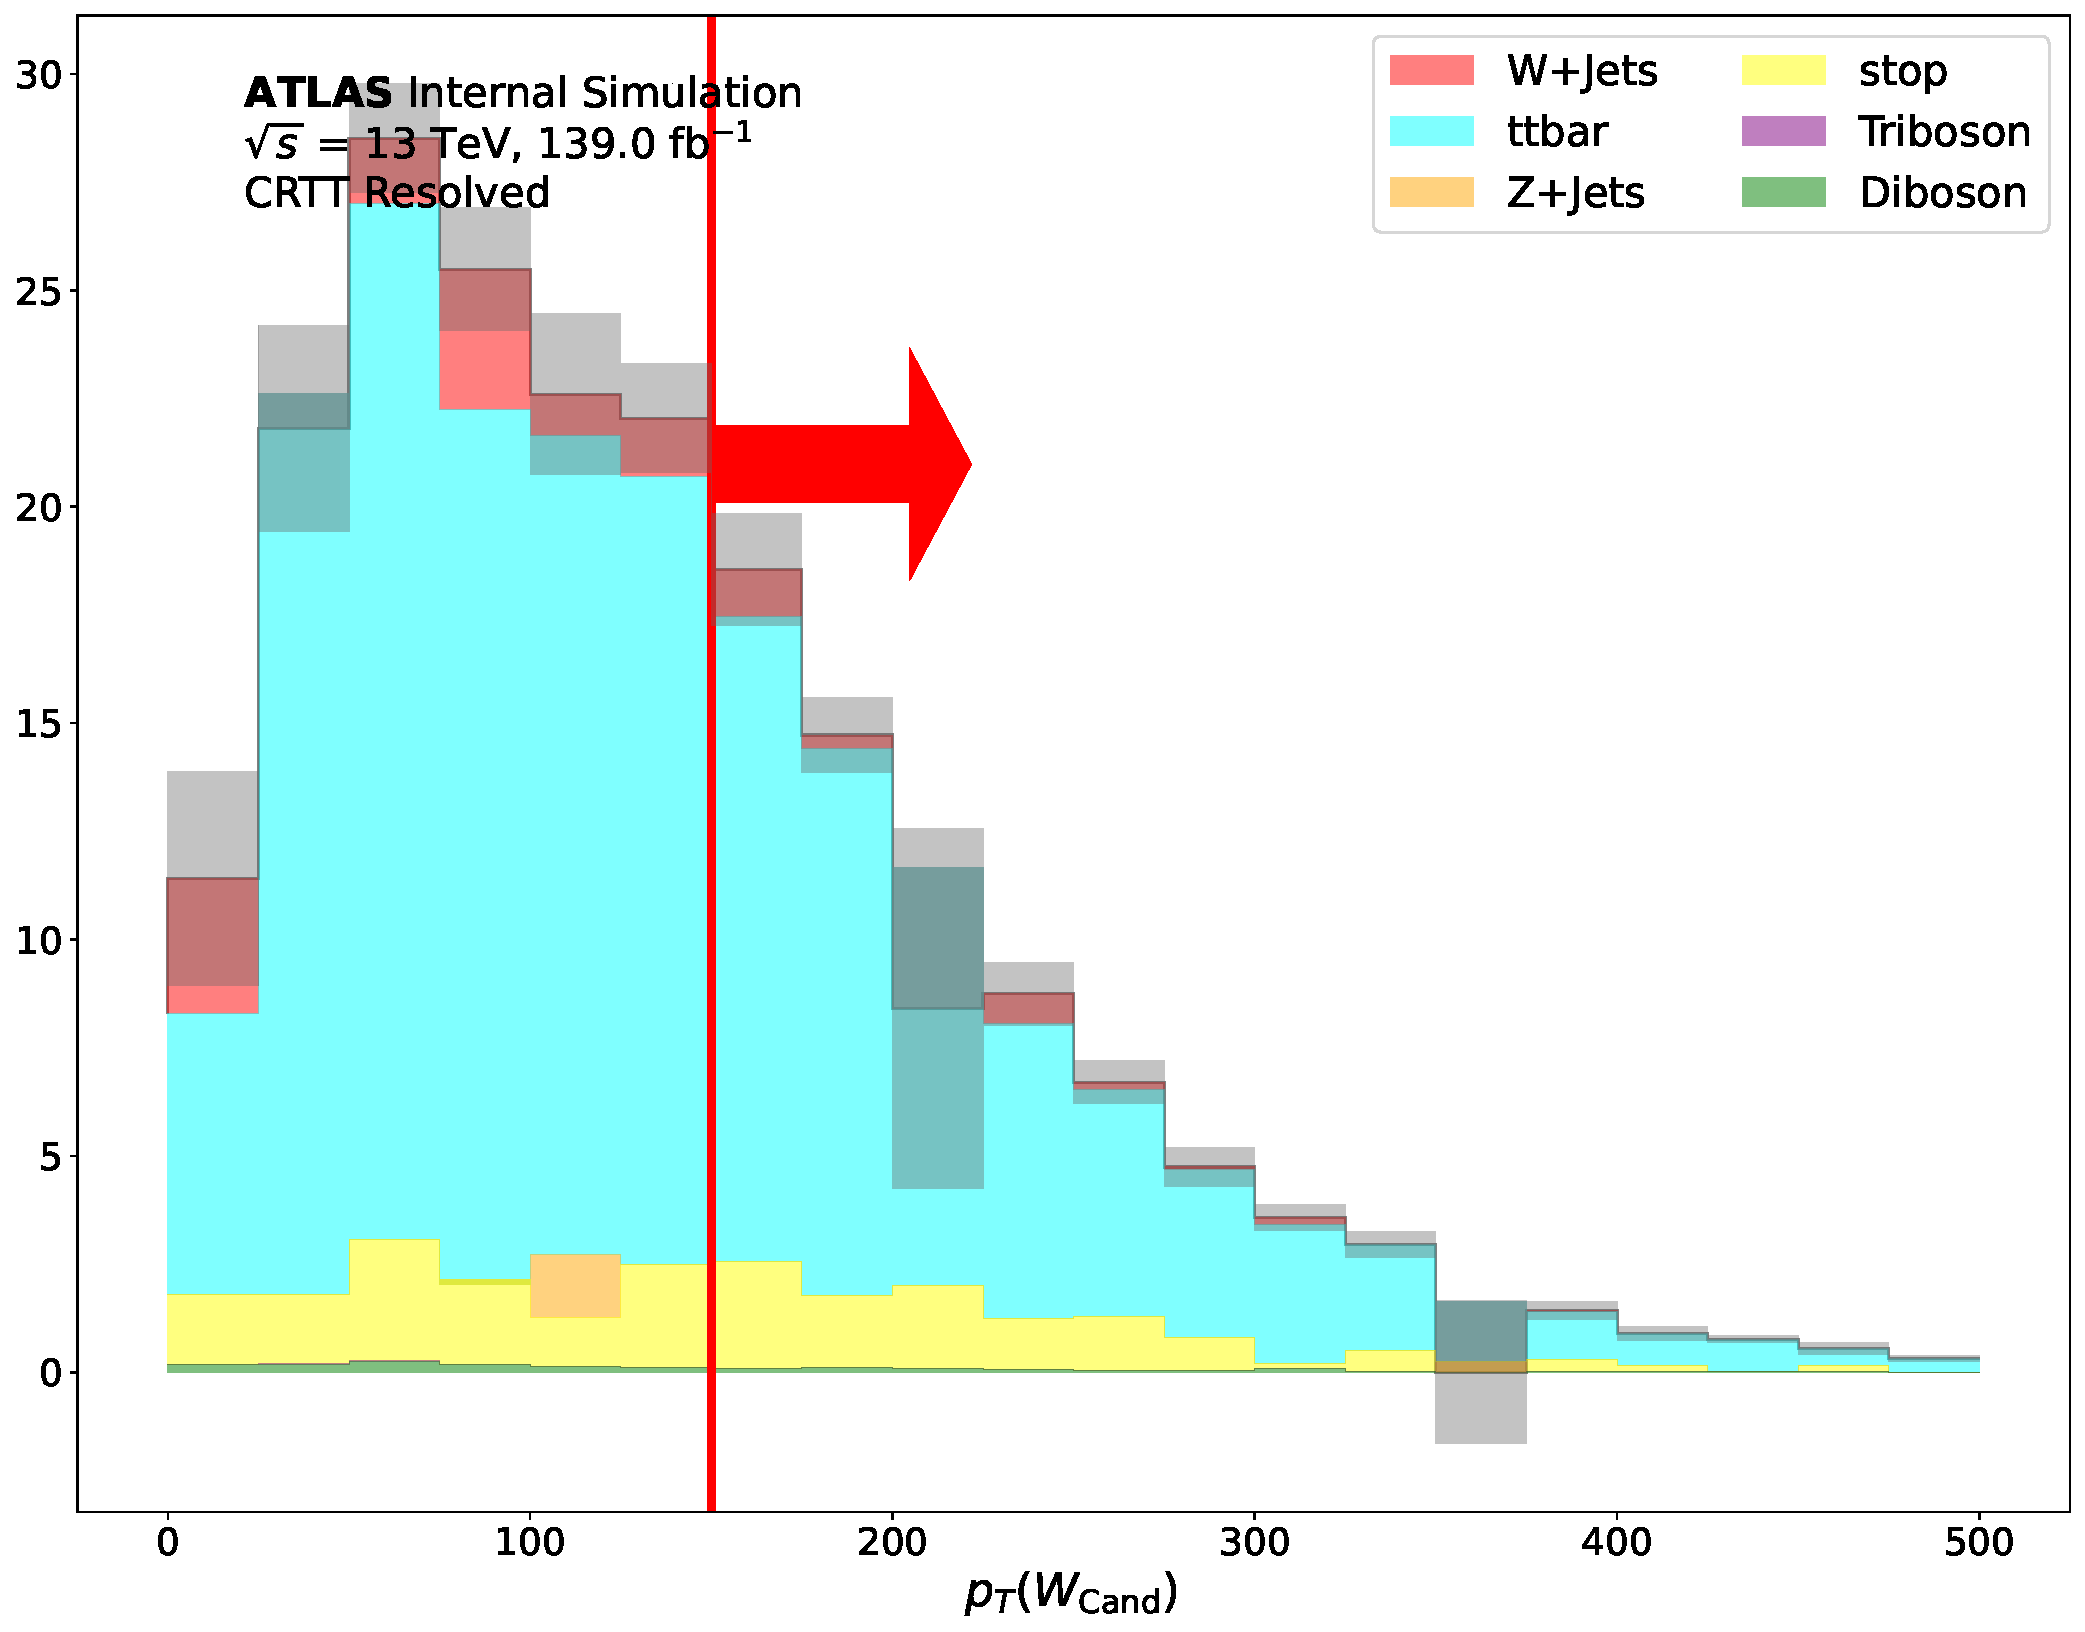
\includegraphics[width = 0.95\textwidth]{Figures/App_SR_CR_distributions/CRTT_Resolved/WCand_pt_N_1.pdf}
     \caption{\Wcandpt (resolved \ttbar CR)}
     \end{subfigure}
     
    \begin{subfigure}{0.45\textwidth}
     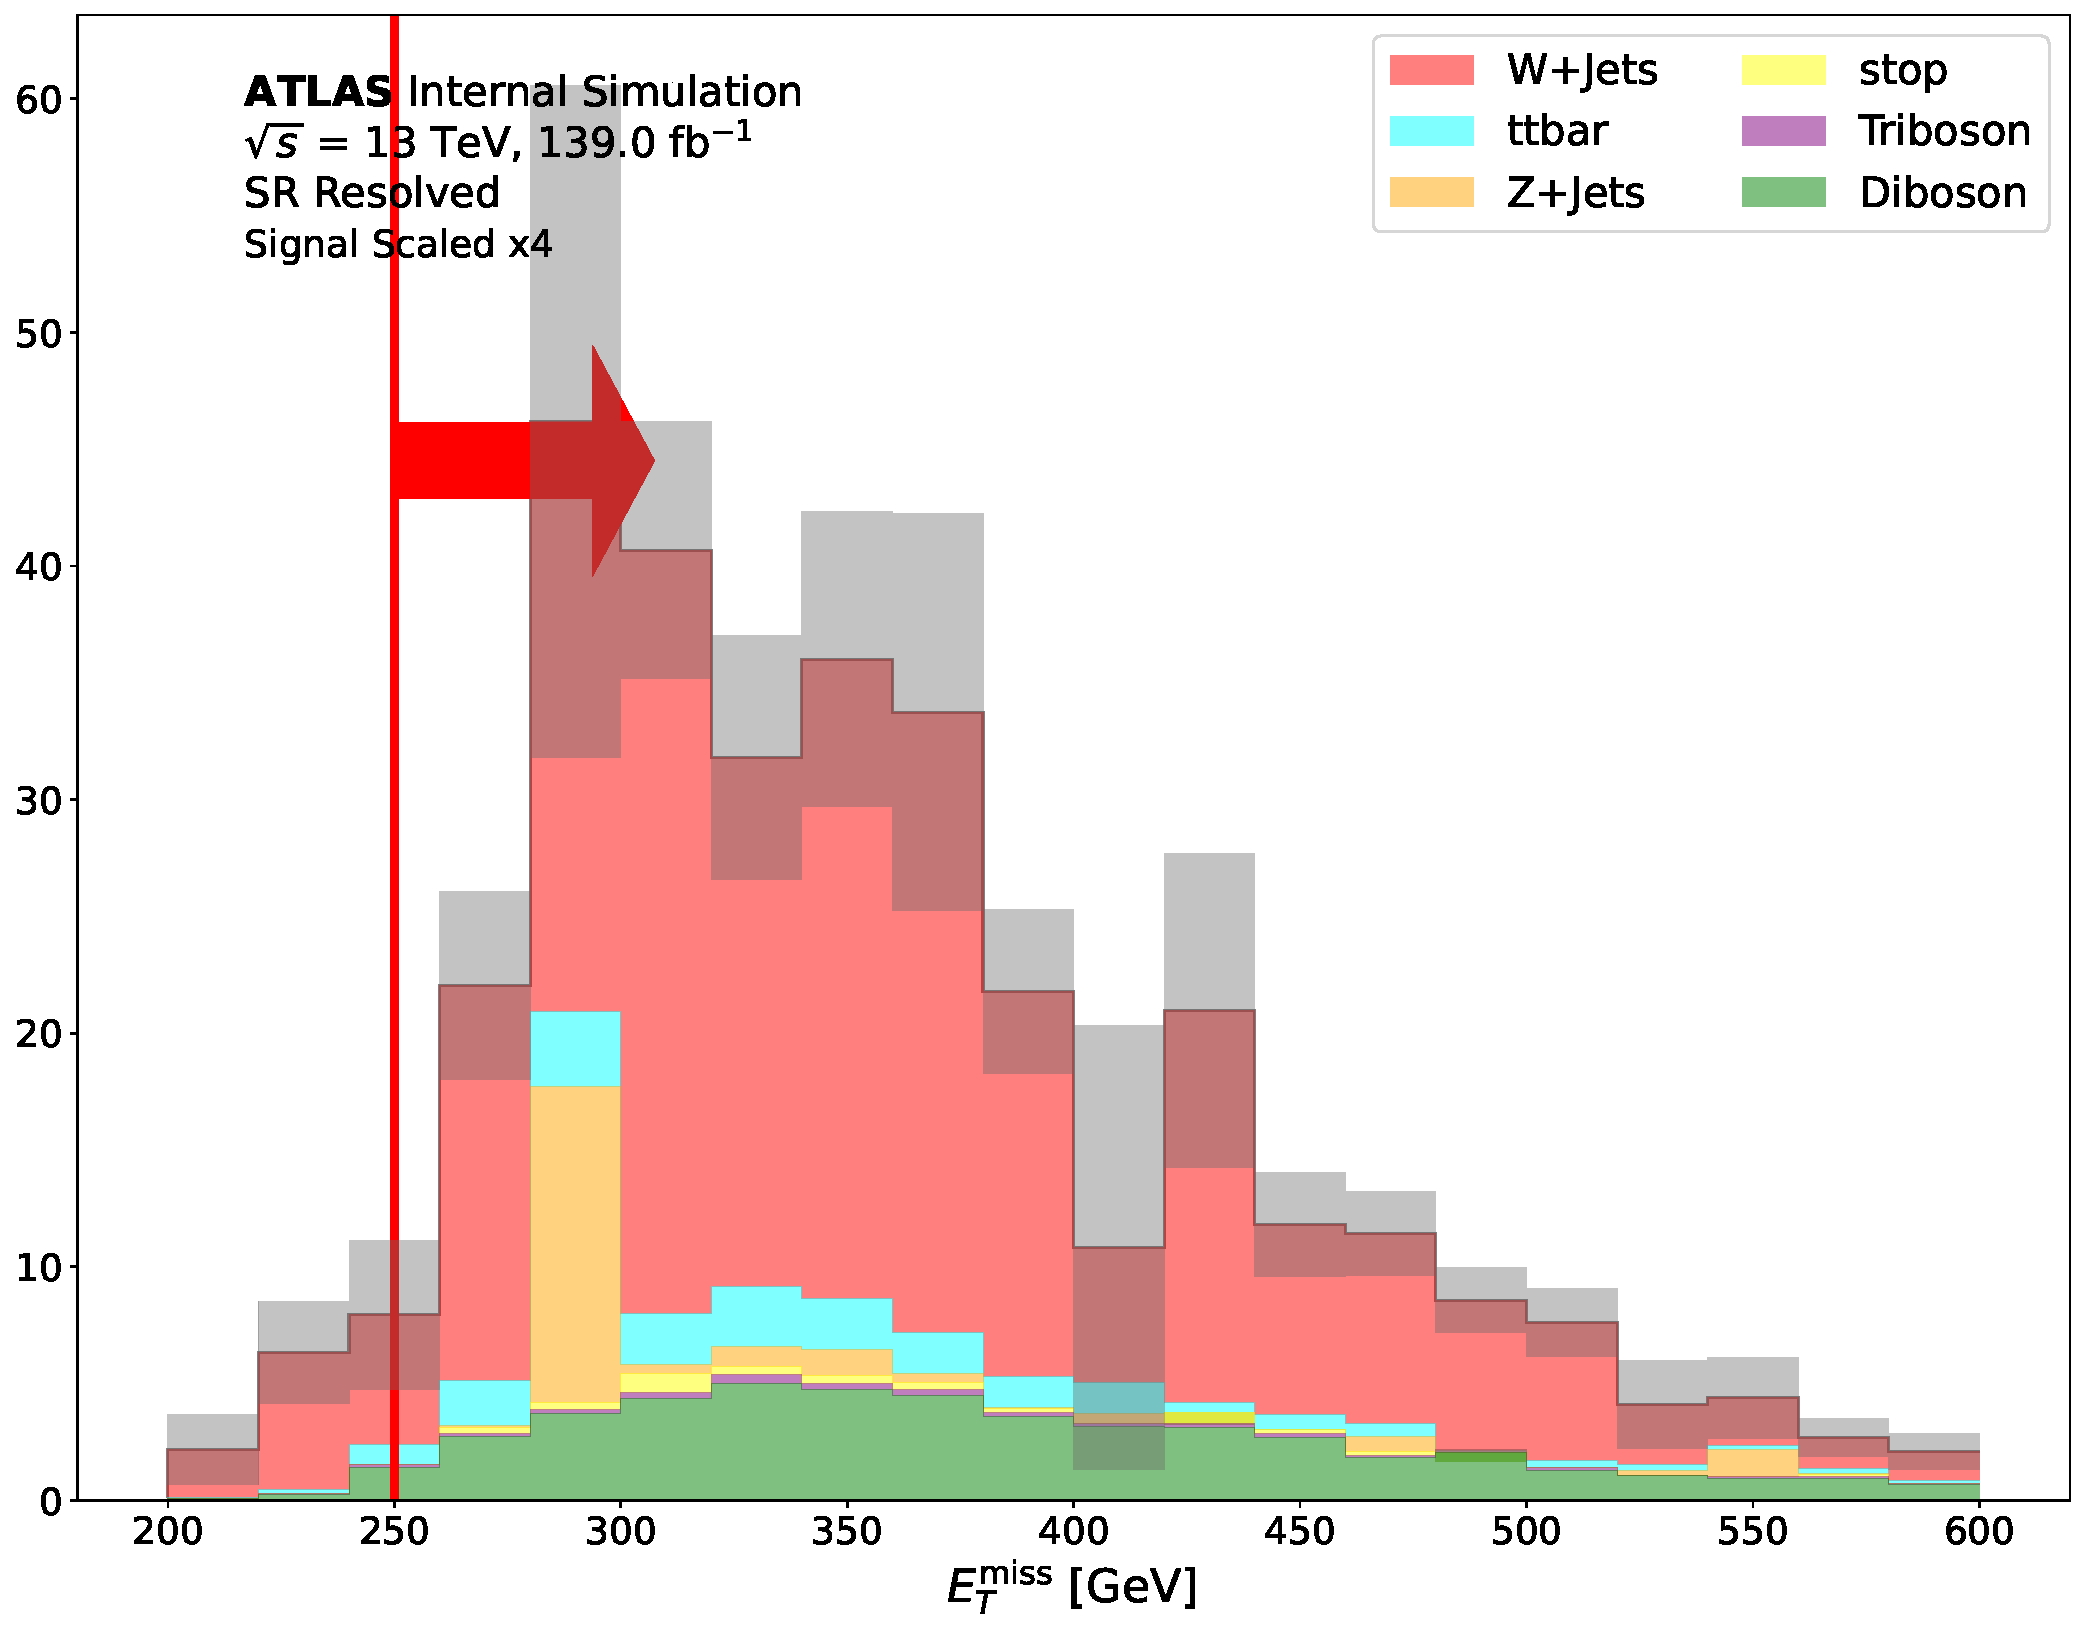
\includegraphics[width = 0.95\textwidth]{Figures/App_SR_CR_distributions/SR1L_Resolved/MetTST_met_N_1.pdf}
    \caption{\met (resolved SR)}
     \end{subfigure}
    \begin{subfigure}{0.45\textwidth}
     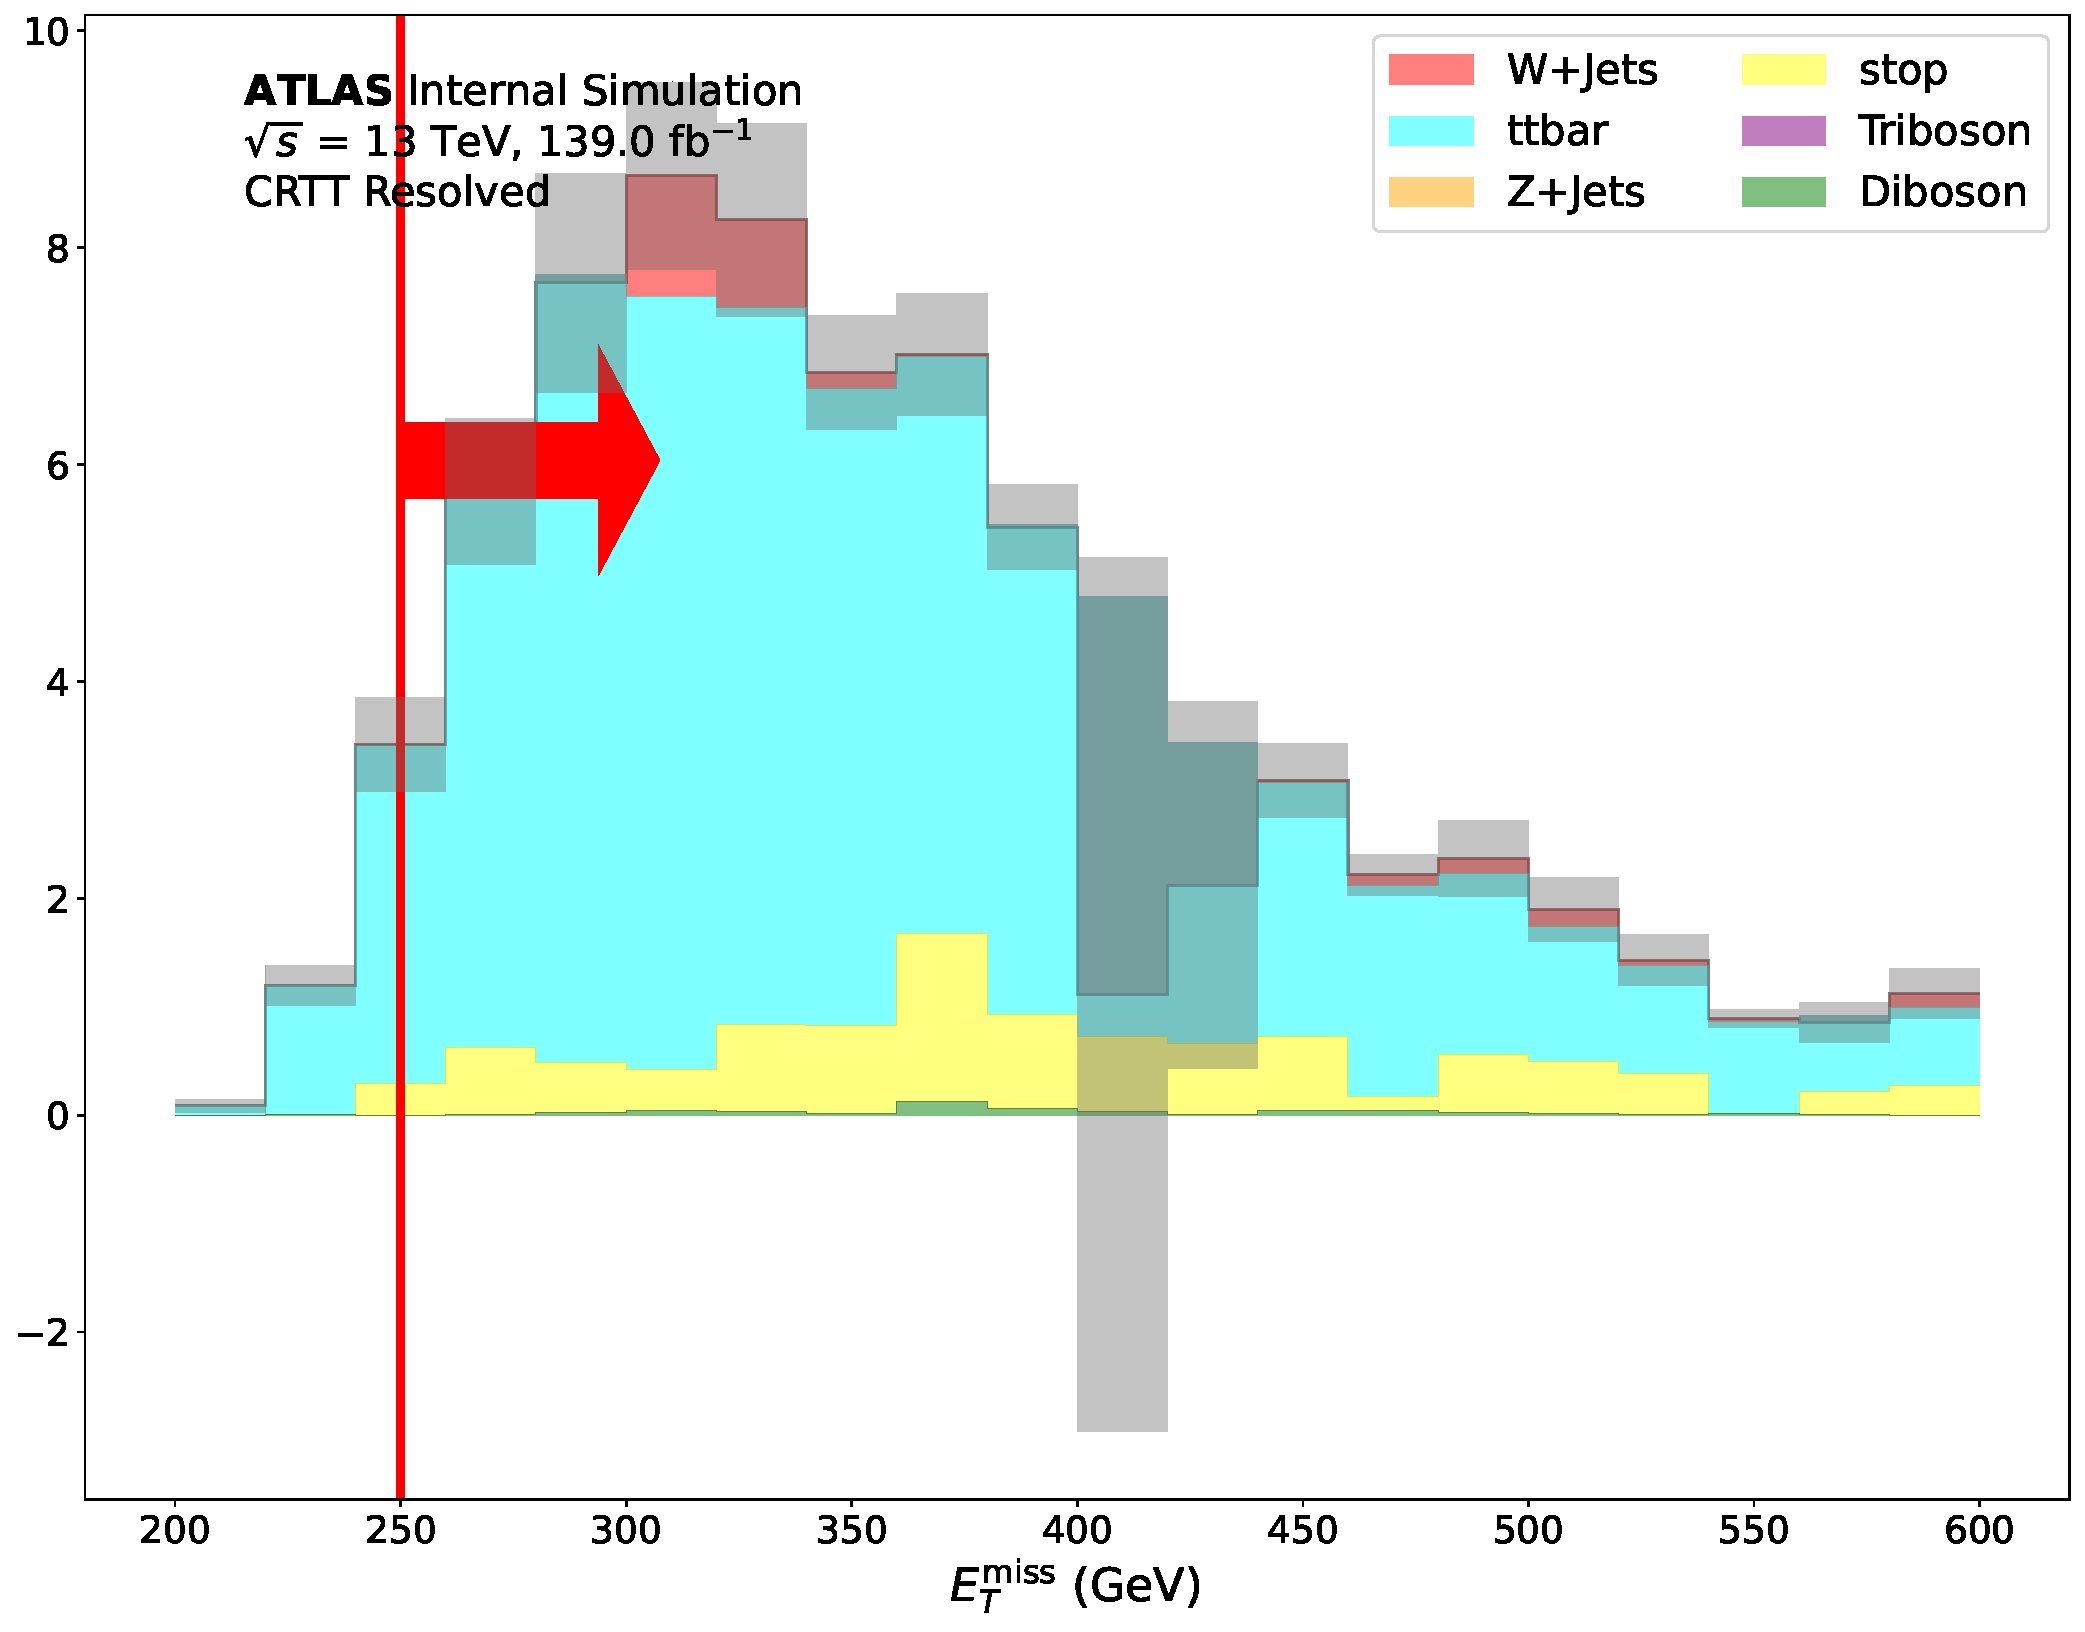
\includegraphics[width = 0.95\textwidth]{Figures/App_SR_CR_distributions/CRTT_Resolved/MetTST_met_N_1.pdf}
     \caption{\met (resolved \ttbar CR)}
     \end{subfigure}

     \caption{Comparison of N-1 distributions for kinematic variables of interest between the SR and the \ttbar CR in the merged category (continued)}
     \label{fig:N_1_CRTT_resolved}
  \end{figure}

